%\documentclass[10pt,a4paper,english]{article}
%DIF LATEXDIFF DIFFERENCE FILE
%DIF DEL ijm - Old original.tex   Tue Jul 24 00:56:13 2018
%DIF ADD ijm.tex                  Tue Jul 24 02:31:48 2018
\documentclass[12pt, a4paper]{article}
\usepackage[utf8]{inputenc}
\usepackage[T1]{fontenc}
%DIF 5c5
%DIF < \usepackage[margin=2.5cm, top=2.5cm, bottom=2.0cm]{geometry}
%DIF -------
\usepackage[margin=2.5cm,top=2.5cm, bottom=2.0cm]{geometry} %DIF > 
%DIF -------
\usepackage[english]{babel}
%\usepackage{lmodern}
\usepackage{newtxtext}
\usepackage{newtxmath}
\usepackage[fleqn]{mathtools}
\usepackage{amssymb}
\usepackage{dcolumn}
%DIF 13a13
\usepackage{siunitx} %DIF > 
%DIF -------
\usepackage[official]{eurosym}
\setcounter{secnumdepth}{3}

\usepackage[babel=true]{microtype}
\usepackage[hang]{footmisc}
\usepackage[usenames,dvipsnames,svgnames,table]{xcolor}

\usepackage[format=hang, justification=RaggedRight]{caption}
\usepackage[section]{placeins}
%DIF 22a23
\usepackage{float} %DIF > 
%DIF -------
\usepackage{booktabs}
\usepackage{comment}
\usepackage{graphicx}
\usepackage{epstopdf}
%DIF 26-27c28-30
%DIF <  
%DIF <  \usepackage[author=, status=draft]{fixme}
%DIF -------
\usepackage[layout=margin,author=,status=draft]{fixme} %DIF > 
 \usepackage[final]{changes} %Manually track changes %DIF > 
 \definechangesauthor{SKB} %DIF > 
%DIF -------
\usepackage{longtable}
\usepackage{paralist}
\usepackage{rotating}
\usepackage{subfigure}
\usepackage[natbibapa]{apacite}
%\usepackage[authoryear]{natbib}
\usepackage{csquotes}
%modifying the thanks commands
\usepackage{titling}
\usepackage[colorlinks=true, urlcolor=blue, citecolor=black, linkcolor=black]{hyperref}
\usepackage[noabbrev,capitalise]{cleveref}

%DIF 40a43
\DeclareUnicodeCharacter{2010}{-}% support older LaTeX versions %DIF > 
%DIF -------
\thanksfootextra{}{\hfill}
\setlength{\thanksmargin}{1em}
\setlength{\thanksmarkwidth}{0.75em}

%DIF 44a48
\fxsetup{theme=color} %DIF > 
%DIF -------
%Custom commands
\newcommand{\eur}{\EUR}
\newcommand{\std}[1]{\emph{(#1)}}
%DIF 47c52
%DIF < \newcommand{\V}{{\ensuremath\checkmark}}
%DIF -------
\newcommand{\V}{\checkmark} %DIF > 
%DIF -------
\def\fns{\footnotesize}
\renewcommand*{\vec}[1]{\boldsymbol{#1}}

\def\tenpc{$^{\ast}$}
\def\fivepc{$^{\ast\ast}$}
\def\onepc{$^{\ast\ast\ast}$}
\newcommand{\legend}{\normalsize{Significance levels:\hspace{1em} \tenpc : 10\% \hspace{1em} \fivepc : 5\% \hspace{1em} \onepc : 1\% \normalsize}}
\def\sep{0.5em}
\def\legendTwo{\multicolumn{3}{l}{\footnotesize{Significance levels
			:\hspace{1em} $\dag$ : 10\% \hspace{1em}
			$\ast$ : 5\% \hspace{1em} $\ast\ast$ : 1\% \normalsize}}}
%DIF 59-60c64-74
%DIF < \renewcommand{\thesection}{\arabic{section}.}
%DIF < \renewcommand{\thesubsection}{\thesection\arabic{subsection}.}
%DIF -------
\def\sym#1{\ifmmode^{#1}\else\(^{#1}\)\fi} % needed for the tables produced by the esttab command in Stata, to avoid redundancy put here instead of in appendix.tex, where it is needed		 %DIF > 
%SKB: Added for documenting the tables and figures %DIF > 
\newcommand{\modelTwo}{age, age\textsuperscript{2}, education, marriage, number of children, inter-ethnic household} %DIF > 
\newcommand{\modelThree}{\modelTwo, industry, occupation, ownership type of company, number of workers in company, working in the public sector, experience in company} %DIF > 
\newcommand{\modelThreeAdd}{industry, occupation, ownership type of company, number of workers in company, working in the public sector, experience in company}	 %DIF > 
\newcommand{\restrictions}{The sample period is from year 2000 to year 2012. Sample is limited to persons 25-55 year old.} %DIF > 
\newcommand{\agerestrictions}{25-55 year olds only.} %DIF > 
% Modified section numbering: removed dot at the end as this jumps %DIF > 
% into the cross-references. %DIF > 
\renewcommand{\thesection}{\arabic{section}} %DIF > 
\renewcommand{\thesubsection}{\thesection.\arabic{subsection}} %DIF > 
%DIF -------

\title{Language Skills in an Ethnically Segmented Labour market:
 Estonia 1989 -- 2012}
%\author{Sven-Kristjan Bormann \and Svetlana Ridala\thanks{Acknowledgements: 
%This research was supported by European Social Fund's Doctoral Studies
%and Internationalisation Program DoRa through Archimedes Foundation, and the Estonian Science Foundation grant 8627.} 
%\and Ott Toomet
%}
\date{}
%DIF PREAMBLE EXTENSION ADDED BY LATEXDIFF
%DIF UNDERLINE PREAMBLE %DIF PREAMBLE
\RequirePackage[normalem]{ulem} %DIF PREAMBLE
\RequirePackage{color}\definecolor{RED}{rgb}{1,0,0}\definecolor{BLUE}{rgb}{0,0,1} %DIF PREAMBLE
\providecommand{\DIFaddtex}[1]{{\protect\color{blue}\uwave{#1}}} %DIF PREAMBLE
\providecommand{\DIFdeltex}[1]{{\protect\color{red}\sout{#1}}}                      %DIF PREAMBLE
%DIF SAFE PREAMBLE %DIF PREAMBLE
\providecommand{\DIFaddbegin}{} %DIF PREAMBLE
\providecommand{\DIFaddend}{} %DIF PREAMBLE
\providecommand{\DIFdelbegin}{} %DIF PREAMBLE
\providecommand{\DIFdelend}{} %DIF PREAMBLE
%DIF FLOATSAFE PREAMBLE %DIF PREAMBLE
\providecommand{\DIFaddFL}[1]{\DIFadd{#1}} %DIF PREAMBLE
\providecommand{\DIFdelFL}[1]{\DIFdel{#1}} %DIF PREAMBLE
\providecommand{\DIFaddbeginFL}{} %DIF PREAMBLE
\providecommand{\DIFaddendFL}{} %DIF PREAMBLE
\providecommand{\DIFdelbeginFL}{} %DIF PREAMBLE
\providecommand{\DIFdelendFL}{} %DIF PREAMBLE
%DIF HYPERREF PREAMBLE %DIF PREAMBLE
\providecommand{\DIFadd}[1]{\texorpdfstring{\DIFaddtex{#1}}{#1}} %DIF PREAMBLE
\providecommand{\DIFdel}[1]{\texorpdfstring{\DIFdeltex{#1}}{}} %DIF PREAMBLE
\newcommand{\DIFscaledelfig}{0.5}
%DIF HIGHLIGHTGRAPHICS PREAMBLE %DIF PREAMBLE
\RequirePackage{settobox} %DIF PREAMBLE
\RequirePackage{letltxmacro} %DIF PREAMBLE
\newsavebox{\DIFdelgraphicsbox} %DIF PREAMBLE
\newlength{\DIFdelgraphicswidth} %DIF PREAMBLE
\newlength{\DIFdelgraphicsheight} %DIF PREAMBLE
% store original definition of \includegraphics %DIF PREAMBLE
\LetLtxMacro{\DIFOincludegraphics}{\includegraphics} %DIF PREAMBLE
\newcommand{\DIFaddincludegraphics}[2][]{{\color{blue}\fbox{\DIFOincludegraphics[#1]{#2}}}} %DIF PREAMBLE
\newcommand{\DIFdelincludegraphics}[2][]{% %DIF PREAMBLE
\sbox{\DIFdelgraphicsbox}{\DIFOincludegraphics[#1]{#2}}% %DIF PREAMBLE
\settoboxwidth{\DIFdelgraphicswidth}{\DIFdelgraphicsbox} %DIF PREAMBLE
\settoboxtotalheight{\DIFdelgraphicsheight}{\DIFdelgraphicsbox} %DIF PREAMBLE
\scalebox{\DIFscaledelfig}{% %DIF PREAMBLE
\parbox[b]{\DIFdelgraphicswidth}{\usebox{\DIFdelgraphicsbox}\\[-\baselineskip] \rule{\DIFdelgraphicswidth}{0em}}\llap{\resizebox{\DIFdelgraphicswidth}{\DIFdelgraphicsheight}{% %DIF PREAMBLE
\setlength{\unitlength}{\DIFdelgraphicswidth}% %DIF PREAMBLE
\begin{picture}(1,1)% %DIF PREAMBLE
\thicklines\linethickness{2pt} %DIF PREAMBLE
{\color[rgb]{1,0,0}\put(0,0){\framebox(1,1){}}}% %DIF PREAMBLE
{\color[rgb]{1,0,0}\put(0,0){\line( 1,1){1}}}% %DIF PREAMBLE
{\color[rgb]{1,0,0}\put(0,1){\line(1,-1){1}}}% %DIF PREAMBLE
\end{picture}% %DIF PREAMBLE
}\hspace*{3pt}}} %DIF PREAMBLE
} %DIF PREAMBLE
\LetLtxMacro{\DIFOaddbegin}{\DIFaddbegin} %DIF PREAMBLE
\LetLtxMacro{\DIFOaddend}{\DIFaddend} %DIF PREAMBLE
\LetLtxMacro{\DIFOdelbegin}{\DIFdelbegin} %DIF PREAMBLE
\LetLtxMacro{\DIFOdelend}{\DIFdelend} %DIF PREAMBLE
\DeclareRobustCommand{\DIFaddbegin}{\DIFOaddbegin \let\includegraphics\DIFaddincludegraphics} %DIF PREAMBLE
\DeclareRobustCommand{\DIFaddend}{\DIFOaddend \let\includegraphics\DIFOincludegraphics} %DIF PREAMBLE
\DeclareRobustCommand{\DIFdelbegin}{\DIFOdelbegin \let\includegraphics\DIFdelincludegraphics} %DIF PREAMBLE
\DeclareRobustCommand{\DIFdelend}{\DIFOaddend \let\includegraphics\DIFOincludegraphics} %DIF PREAMBLE
\LetLtxMacro{\DIFOaddbeginFL}{\DIFaddbeginFL} %DIF PREAMBLE
\LetLtxMacro{\DIFOaddendFL}{\DIFaddendFL} %DIF PREAMBLE
\LetLtxMacro{\DIFOdelbeginFL}{\DIFdelbeginFL} %DIF PREAMBLE
\LetLtxMacro{\DIFOdelendFL}{\DIFdelendFL} %DIF PREAMBLE
\DeclareRobustCommand{\DIFaddbeginFL}{\DIFOaddbeginFL \let\includegraphics\DIFaddincludegraphics} %DIF PREAMBLE
\DeclareRobustCommand{\DIFaddendFL}{\DIFOaddendFL \let\includegraphics\DIFOincludegraphics} %DIF PREAMBLE
\DeclareRobustCommand{\DIFdelbeginFL}{\DIFOdelbeginFL \let\includegraphics\DIFdelincludegraphics} %DIF PREAMBLE
\DeclareRobustCommand{\DIFdelendFL}{\DIFOaddendFL \let\includegraphics\DIFOincludegraphics} %DIF PREAMBLE
%DIF END PREAMBLE EXTENSION ADDED BY LATEXDIFF

\begin{document}

%\maketitle
%\begin{center}
%	\textbf{{\large Language Skills in an Ethnically Segmented Labour market:
%				Estonia 1989 -- 2012}} \\
%	{\large Sven-Kristjan Bormann} \\
%	\emph{School of Economics and Business Administration, University of Tartu, Narva mnt. 4, 51007 Tartu, Estonia\\ Tel.: +372 5844 3873\\ Email: \href{mailto:bormann@ut.ee}{bormann@ut.ee}}	\\
%
%	{\large Svetlana Ridala} \\
%	\emph{School of Business and Governance, Tallinn University of Technology, Akadeemia tee 3, 12618 Tallinn, Estonia\\ Email: \href{
%			mailto:svetlana.ridala@gmail.com}{
%			svetlana.ridala@gmail.com}} \\
%		{\large Ott Toomet}\\
%		\emph{Information School, University of Washington, USA; Email: \href{mailto:otoomet@uw.edu}{otoomet@uw.edu}}
%%	\emph{(Received XX XXXX 20XX; accepted XX XXXX 20XX)}\\
%	\textbf{Corresponding author:} Sven-Kristjan Bormann Email: \href{mailto:bormann@ut.ee}{bormann@ut.ee}
%\end{center}
%\paragraph{Short biographical note:} \hspace{0pt} \\
%Sven-Kristjan Bormann born 28.11.1985, graduated in 2011 from Kiel University, Germany in Economics with specialisation in Quantitative Economics and Computer Science. Since September 2012 PhD-student in Economics at Tartu University, Estonia. \\
%Svetlana Ridala born 28.03.1976, graduated in 2003 from Tallinn Pedagogical University, Estonia master's (scien) degree in mathematics. Since 2009 PhD-student in Economics at Tallinn School of Economics and Business Administration, Estonia.
%\\
%Ott-Siim Toomet born 18.03.1970, graduated in 2004 from Aarhus University, Denmark PhD in Economics. Since 2015 Visiting scholar, Information School, University of Washington.
%
%\paragraph{Research funding}
%This research was supported by European Social Fund's Doctoral Studies
%and Internationalisation Program DoRa through Archimedes Foundation, and the Estonian Science Foundation grant 8627.
%\newpage
%\noindent
{\centering \textbf{Language Skills in an Ethnically Segmented Labour \DIFdelbegin \DIFdel{market}\DIFdelend \DIFaddbegin \DIFadd{Market}\DIFaddend : Estonia 1989 -- 2012}}
\begin{abstract}
 \DIFdelbegin %DIFDELCMD < 

%DIFDELCMD < 	%%%
\DIFdelend \noindent
 \textbf{Purpose --} \DIFdelbegin \DIFdel{The purpose of this paper is to study }\DIFdelend \DIFaddbegin \DIFadd{We analyse }\DIFaddend the relationship between \DIFdelbegin \DIFdel{language skills and }\DIFdelend \DIFaddbegin \DIFadd{skills in the
 Estonian, Russian and English language, and }\DIFaddend labour market
 outcomes in Estonia, a linguistically divided country\DIFdelbegin \DIFdel{where Estonian
is the sole official language}\DIFdelend .
 \\
 \textbf{Design/methodology/approach --} \DIFdelbegin \DIFdel{The authors }\DIFdelend \DIFaddbegin \DIFadd{We }\DIFaddend use the Estonian Labour
 Force \DIFdelbegin \DIFdel{Survey from 1989 to 2012 to study the impact of language skills on unemployment (probability) and
 wages}\DIFdelend \DIFaddbegin \DIFadd{Surveys 1992--2012. We rely on multivariate linear regression
 models to document the relationship between language skills and
 labour market outcomes}\DIFaddend .
 \\
 \textbf{Findings --} \DIFdelbegin \DIFdel{For men, fluency in Estonian is
 related to approximately 5 percentage points lower unemployment, but to virtually no income
premium. English skills are associated with a
substantial income premium , but are virtually unrelated to
unemployment. Russian skills are related to higher wages for Estonians, but the premium is falling over time and Russian is not associated with lower unemployment}\DIFdelend \DIFaddbegin \DIFadd{Estonian language knowledge (for ethnic Russians)
 are important determinants of unemployment. Wage, in contrary, is
 closely related to English skills. Ethnic Russian men do not earn
 any premium from speaking Estonian, while women, fluent in Estonian
 earn approximately 10\% more. For ethnic Estonians, Russian fluency
 is associated with a similar income gain}\DIFaddend .
 \\
 \textbf{Research limitations/implications -- } \DIFdelbegin \DIFdel{No casual claims are possible unless a suitable instruments for language skills can be found. Individual characteristics are able to explain a
large part of English returns, so that part of the remaining effect
may also be related to an ability bias. The usage of }\DIFdelend \DIFaddbegin \DIFadd{Due to the
 observational nature of the data, the effects reported in our study
 are not causal effects. As a second limitation, the }\DIFaddend self-reported
 language skills \DIFdelbegin \DIFdel{may introduce measurement errors, which may	decrease in the future, as language test data becomes available}\DIFdelend \DIFaddbegin \DIFadd{data may be imprecise and hence the effects we
 report may be too small}\DIFaddend .
 \\
 \textbf{Practical implications --} \DIFdelbegin \DIFdel{These results can be explained by simultaneous ethnic and gender
segregation where the high-skilled male labour market is more segregated
than the female labour market, and females are more often working in
 communication-intensive jobs}\DIFdelend \DIFaddbegin \DIFadd{Our results stress the role of
 workplace segregation, both along gender and ethnic lines, in
 determining the individual labour market experience}\DIFaddend . 
 \\
 \textbf{Originality/value --} \DIFdelbegin \DIFdel{This paper provides }\DIFdelend \DIFaddbegin \DIFadd{We provide }\DIFaddend a comprehensive overview \DIFdelbegin \DIFdel{about }\DIFdelend \DIFaddbegin \DIFadd{of
 }\DIFaddend the effects of language skills \DIFdelbegin \DIFdel{on labour
 market outcomes for }\DIFdelend \DIFaddbegin \DIFadd{in a rapidly developing labour
 market in }\DIFaddend a linguistically divided \DIFdelbegin \DIFdel{, low immigration population. In contrast, the existing literature deals mostly with the effects of language skills on the labour market outcomes of immigrants}\DIFdelend \DIFaddbegin \DIFadd{economy. We analyse several
 languages with different legal status and document long-term
 trends in the effects}\DIFaddend .
 \\
\end{abstract}
\textbf{Keywords:} language skills, ethnicity, wage gap, unemployment, Estonia \\
\textbf{JEL classification:} J15, J31, J71


\section{Introduction}
\label{sec:introduction}
Numerous studies document that language skills are related to better
labour market outcomes.
Speaking different languages may make workers genuinely more
productive, either by facilitating communication at the workplace
or by making it possible to perform
tasks that require language knowledge.
Enhanced productivity, in turn, should be reflected both in better wage
and in improved employment prospects.

The bulk of the existing literature analyses the effect of knowledge
of the local majority language for immigrants. It is well known that
language skills are associated with \DIFdelbegin \DIFdel{a substantial }\DIFdelend an income premium
between 5 and 35 percent
\DIFdelbegin %DIFDELCMD < \citep{Chiswick1995,bleakley+chin2004,shields+price2002,leslie+lindley2001,chiswick+miller2002,Chiswick2003,Chiswick2010,Chiswick2015, Dustmann2003}%%%
\DIFdelend \DIFaddbegin \citep{Chiswick1995,bleakley+chin2004,shields+price2002,leslie+lindley2001,chiswick+miller2002,Chiswick2010,Chiswick2015, Dustmann2003}\DIFaddend . For
instance, \citet{chiswick2008} argues that ``proficient'' speakers
typically earn about 15\% more than ``not proficient'' speakers.
The effect works largely through improving educational attainment
\citep{bleakley+chin2004,rooth+saarela2007native}. Language skills are
also complementary to other types of human capital
\citep{chiswick+miller2007}.
Immigrants who are fluent in the local language also suffer
substantially less from unemployment \citep{shields+price2002, Dustmann2003}.



However, in case of less-than-perfect ethnic integration, the ``local''
language in ethnic enclaves may be the minority language instead, in
this way limiting the usefulness of the majority language skills
\citep{chiswick+miller2002,hwang+2010} in particular in context of ethnic segregation and
limited access to upper-end jobs \citep{Toomet2011}. However, the
existing evidence suggests that the majority language is
an important production factor in the ethnic enclaves as well
\citep{zhou+logan1989, clark+drinkwater2000}.


There is also an increasing body of literature focusing on \DIFdelbegin \DIFdel{relationship
between }\DIFdelend other languages than the local main business language\DIFdelbegin \DIFdel{and
income}\DIFdelend . These studies generally find
that English is a significant predictor of better income
\DIFdelbegin %DIFDELCMD < \citep{Lang2009, Casale2011, Toomet2011, Williams2011, azam+2013EDandCC, isphording2013, beblavy+2016CEPS}%%%
\DIFdel{.
}%DIFDELCMD < 

%DIFDELCMD < %%%
\DIFdelend \DIFaddbegin \citep{Lang2009, Casale2011, Toomet2011, Williams2011, azam+2013EDandCC, isphording2013, fabo+2017E}\DIFadd{.
}\DIFaddend The role of other languages\DIFaddbegin \DIFadd{, in particular in multi-lingual economy, }\DIFaddend is
less clear. \DIFdelbegin \DIFdel{It is especially unclear what is the role of
different languages in a multi-lingual economy.  }\DIFdelend For instance,
\cite{Drinkwater1997} finds
a positive effect for Welsh speaking workers in
Wales \DIFdelbegin \DIFdel{but }\DIFdelend \DIFaddbegin \DIFadd{and \mbox{%DIFAUXCMD
\cite{Armstrong2015} }\hspace{0pt}%DIFAUXCMD
shows that bilingual native French-speakers enjoy
a significant premium both inside and outside of Quebec.
}\DIFaddend \citet{FrancoisGrin1998}, in contrast,
shows that Italian language skills in Swiss non-Italian speaking
regions are associated with \DIFaddbegin \DIFadd{a }\DIFaddend lower wage. It remains unclear if
this is a true effect or just an omitted variable bias.
\DIFdelbegin \DIFdel{It is estimated by \mbox{%DIFAUXCMD
\cite{Armstrong2015} }\hspace{0pt}%DIFAUXCMD
that there is a statistically significant premium paid to bilingual people both inside and outside Quebec who speak French as their mother tongue People speaking English as their mother tongue also earn a premium, but it is much smaller outside of Quebec. In some cases it is even statistically not significant.
}\DIFdelend 

Few previous studies have provided a comprehensive analysis of a labour
market from the viewpoint of language skills.
\citet{Chiswick1995, chiswick+miller2002, chiswick+miller2007,
 Bellante1998, Chiswick2010} analyse the effects of dominant language
fluency for earnings among immigrants in the United States\DIFdelbegin \DIFdel{and
}\DIFdelend \DIFaddbegin \DIFadd{, 
}\DIFaddend \citet{Chiswick1995} also \DIFdelbegin \DIFdel{analyse it }\DIFdelend \DIFaddbegin \DIFadd{do this }\DIFaddend for Canada, Australia and Israel.
\DIFdelbegin %DIFDELCMD < \citet{Dustmann2003, shields+price2002} %%%
\DIFdel{explore of immigrant assimilation into the labour market of the United Kingdom.
}%DIFDELCMD < 

%DIFDELCMD < %%%
\DIFdelend \citet{leslie+lindley2001} analyse both employment and income but
focus on a single year and English language only.
\citet{YaoandOurs2015} only analyse the role of Dutch language
on labour market performance in \DIFdelbegin \DIFdel{Netherlands}\DIFdelend \DIFaddbegin \DIFadd{the Netherlands. 
}

\DIFadd{The literature on Central Eastern Europe (CEE) and former Soviet Union
countries is rather limited. We know that the different development
trajectories have led to disparities both favouring Russian-speaking
minority in Ukraine }\citep{Constant2011} \DIFadd{and hindering them in Estonia
}\citep{Leping2008}\DIFaddend . \DIFdelbegin \DIFdel{In case of Estonia
,
}%DIFDELCMD < \citet{Toomet2011} %%%
\DIFdel{shows that the majority language gives little wage
premium for minority men. However, he analyses neither women, nor
unemployment. }\DIFdelend \DIFaddbegin \citet{Kahanec2009} \DIFadd{show that non-citizens suffer
less favourable outcomes, in particular, ethnic Russians in Estonia and
Latvia. 
\mbox{%DIFAUXCMD
\cite{Alan2015} }\hspace{0pt}%DIFAUXCMD
show that Russian language proficiency is valuable in
the former USSR republic in the Caucasus (Armenia, Azerbaijan and
Georgia) by increasing employment likelihood between six and nine
percentage points. }\citet{Toomet2011}\DIFadd{, however, fails to find any
income premium from the majority language fluency in Estonia and
Latvia. This outcome is corroborated by }\DIFaddend \citet{Lindemann2013} \DIFaddbegin \DIFadd{who }\DIFaddend shows that Estonian fluency
is associated with faster job finding rate while \DIFdelbegin \DIFdel{while }\DIFdelend it does not
explain the lower occupational prestige of Russian speakers. 
\DIFdelbegin \DIFdel{However,
she only includes recent school graduates in
her study.
}%DIFDELCMD < \\
%DIFDELCMD < %%%
\DIFdelend \DIFaddbegin \DIFadd{A number of these studies have to overcome severe data limitations,
such as lack of fine-grained information on ethnic background in
EU-wide surveys }\citep{Kahanec2010}\DIFadd{.
}\DIFaddend 

\DIFdelbegin %DIFDELCMD < \noindent %%%
\DIFdelend In this paper, we analyse the relationship between both
majority and minority language skills, and English for both
wage and unemployment. We analyse Estonia, a \DIFdelbegin \DIFdel{linguistically divided
countrywhere a large }\DIFdelend \DIFaddbegin \DIFadd{former Soviet republic
and now a rapidly growing and
transforming Easter European country. It is characterized by a stark linguistic division
where the }\DIFaddend Russian-speaking community forms almost 30\% of
the population. We \DIFaddbegin \DIFadd{use Estonian Labour Force Survey, one of the
higher-quality long-term datasets, well suitable for our
purpose. We }\DIFaddend provide long--term trends from the last years
of the planned economy in 1989 till the post-recession time in 2012.

We find that \DIFdelbegin \DIFdel{in case of, Estonian language}\DIFdelend \DIFaddbegin \DIFadd{the Estonian language, the majority and the official
language of the country, }\DIFaddend is associated with \DIFaddbegin \DIFadd{a }\DIFaddend very
small albeit slowly increasing wage premium over
the years\DIFdelbegin \DIFdel{, but }\DIFdelend \DIFaddbegin \DIFadd{. Interestingly, this is true }\DIFaddend only for women\DIFaddbegin \DIFadd{, Russian men enjoy
virtually no premium from the majority language skills}\DIFaddend .
Russian skills, on the other hand, are clearly related to
higher wage but the relationship is slowly fading. English fluency was
associated with a very large wage premium during the \DIFdelbegin \DIFdel{first decade
after the introduction of
the market economy, it's importance later declined, but was still large in 2012.  For
women, the wage premium of each of these languages is roughly equal}\DIFdelend \DIFaddbegin \DIFadd{early years of
economic transition, later its importance
declined but remained sizeable}\DIFaddend . 
In contrast, the sole language that plays a role in determining
unemployment \DIFdelbegin \DIFdel{is Estonian, it's }\DIFdelend \DIFaddbegin \DIFadd{probability is Estonian. Its }\DIFaddend fluency is associated with 
approximately 5 percentage points lower \DIFdelbegin \DIFdel{unemployment rate}\DIFdelend \DIFaddbegin \DIFadd{probability of being unemployed}\DIFaddend .
These results suggest that \DIFaddbegin \DIFadd{the }\DIFaddend Estonian labour market is 
segmented both along gender and the \DIFdelbegin \DIFdel{ethnic boundaries, }\DIFdelend \DIFaddbegin \DIFadd{along ethnic background, with }\DIFaddend men
more likely occupied in less communication-intense jobs.
\DIFdelbegin \DIFdel{This view is
supported by data from a specifically designed ethnic integration
dataset.
}\DIFdelend 


The paper continues as follows: The next section provides a brief
background of Estonian society and \DIFaddbegin \DIFadd{the }\DIFaddend labour market. In the following
section\DIFaddbegin \DIFadd{, }\DIFaddend we discuss the data and provide some descriptive
statistics. In \cref{sec:method} we describe the econometric
approach, sections \ref{sec:results} and \ref{sec:extensions} present
the results for unemployment probability and wages. \DIFaddbegin \DIFadd{The two last
sections, \ref{sec:segregation-analysis} and \ref{sec:discussion}, are
devoted to an additional analysis of labour market segregation, and
concluding discussion.
}\DIFaddend 


\section{Background: Ethnic Groups and Languages in Estonia}
\label{sec:hist_background}

This section briefly reviews \DIFdelbegin \DIFdel{Estonian institutional background,
}\DIFdelend \DIFaddbegin \DIFadd{the institutional and economic background
in Estonia, a country of 1.3M inhabitants,
}\DIFaddend focusing on the role of ethnic groups and languages.
See \citet{Leping2008} and
\citet{lindemann+saar2011Russian2ndGeneration} for more \DIFaddbegin \DIFadd{detailed }\DIFaddend information.

Before the Second World War, \DIFdelbegin \DIFdel{Estonia }\DIFdelend \DIFaddbegin \DIFadd{the country }\DIFaddend was ethnically rather
homogeneous \DIFdelbegin \DIFdel{, populated almost exclusively by }\DIFdelend \DIFaddbegin \DIFadd{with 90 percent of the population being }\DIFaddend ethnic Estonians. After the War,
the Russian-speaking population grew rapidly through migration and
reached 40\% by 1989. \DIFaddbegin \DIFadd{The migrants largely settled in Ida-Virumaa, a
mineral-rich industrial area in North-East of the country, and in the
metropolitan area near the capital city Tallinn. The
Russian-speakers are still very unevenly distributed.
}

\DIFaddend Such an influx of mainly
Russian-speaking population
led to two \emph{de facto} official languages
by 1970s.
The society was largely divided across language, and the division was
also reflected at workplace \citep{leppik+vihalemm2015JofBaltStud}.
\DIFdelbegin %DIFDELCMD < 

%DIFDELCMD < %%%
\DIFdelend Certain sectors in the economy, such as the \DIFdelbegin \DIFdel{army}\DIFdelend \DIFaddbegin \DIFadd{armed forces}\DIFaddend , railways and the
merchant fleet
were dominated by
Russian-speaking workers while more local industries,
such as agriculture and
\DIFdelbegin \DIFdel{local }\DIFdelend public administration,
were dominated by ethnic Estonians.
Both communities followed the media in their own respective language, the
universities taught many subjects in \DIFaddbegin \DIFadd{both }\DIFaddend Russian and Estonian,
and service sector was largely bilingual. However, the bilingualism
was mainly one-sided as the bulk of Estonians spoke Russian, but not
the other way around. A particular institution in parts of the Soviet
Union was \DIFaddbegin \DIFadd{a }\DIFaddend segregated school system, where Russian schools existed along the
schools teaching in the local language. Hence\DIFaddbegin \DIFadd{, }\DIFaddend a common education
system, one of the central integration mechanisms in the developed world,
was (and still largely is) missing in Estonia.
The widening use of Russian also
caused increasing concerns about the future of the Estonian
language, in turn leading to \DIFaddbegin \DIFadd{an }\DIFaddend unwillingness to use Russian by
the ethnic Estonians. This further strengthened the language-based segregation.

When the central Soviet authority weakened during the late \DIFdelbegin \DIFdel{1980}\DIFdelend \DIFaddbegin \DIFadd{1980s}\DIFaddend , the
Estonian-speaking community was quick to organize and \DIFdelbegin \DIFdel{establish }\DIFdelend \DIFaddbegin \DIFadd{established }\DIFaddend a
nation-state in 1991 where
Estonian was granted status as the sole official language. The
above-mentioned ``one-sided bilingualism'' \DIFdelbegin \DIFdel{slowly }\DIFdelend started turning
around. The universities quickly moved to Estonian-only curriculum,
\DIFdelbegin \DIFdel{Estonian language become a large-scale }\DIFdelend \DIFaddbegin \DIFadd{the Estonian language became a }\DIFaddend compulsory subject in Russian schools
while teaching Russian in Estonian-language schools declined.
\DIFdelbegin \DIFdel{Since 2007, all Russian high-schools have to teach part of the
curriculum in Estonian }%DIFDELCMD < \citep{lindemann+saar2011Russian2ndGeneration}%%%
\DIFdelend \DIFaddbegin \DIFadd{These trends have continued until today, according to
}\citet{HTM2015}\DIFadd{, one quarter of the students from non-Estonian-speaking families studied in Estonian schools}\DIFaddend .
\DIFdelbegin %DIFDELCMD < 

%DIFDELCMD < %%%
\DIFdel{According to the report of the Ministry of Education and Research the number
of students, whose mother tongue is not Estonian in basic schools who study in the Estonian language increased from 17,5\% in 2005 to
25, 8\% in 2015 due to the growing popularity of immersion
classes (enrolment of classes rose from 7,8\% in 2005 to 17,5\% in 2015).
At the same time the number of students whose mother tongue is not Estonian studying in Estonian basic schoolsslowly dropped respectively from 9,5\% to  8,3\% }%DIFDELCMD < \citep{HTM2015}%%%
\DIFdel{.
}%DIFDELCMD < 

%DIFDELCMD < %%%
\DIFdel{The }\DIFdelend \DIFaddbegin \DIFadd{As a result, the }\DIFaddend younger generation of ethnic Estonians is
increasingly less fluent in Russian while the \DIFdelbegin \DIFdel{opposite is true for ethnic Russians . As
a bi-product of the rapid integration to the West, the importance of English language rose
substantially.
}%DIFDELCMD < 

%DIFDELCMD < %%%
\DIFdel{As a result of the }\DIFdelend \DIFaddbegin \DIFadd{ethnic Russians are
steadily getting better in Estonian.
}

\DIFadd{The Estonian economy, a part of the Soviet economy up to 1991, successfully
re-oriented to the Western markets and has been growing rapidly since
the mid-1990s. 
\mbox{%DIFAUXCMD
\Cref{fig:gdp_growth} }\hspace{0pt}%DIFAUXCMD
shows that grew averaged at approximately 7\%
annually
before the financial crisis in 2008, afterwards the figure has been around 3\%.
As a by-product of the re-adjustment, English skills become extremely
valuable while the supply was still rather limited during the early
years of transition.
}

\begin{figure}[h]
 \centering           
 \caption{\DIFaddFL{Annual GDP growth in Estonia}}\label{fig:gdp_growth}
 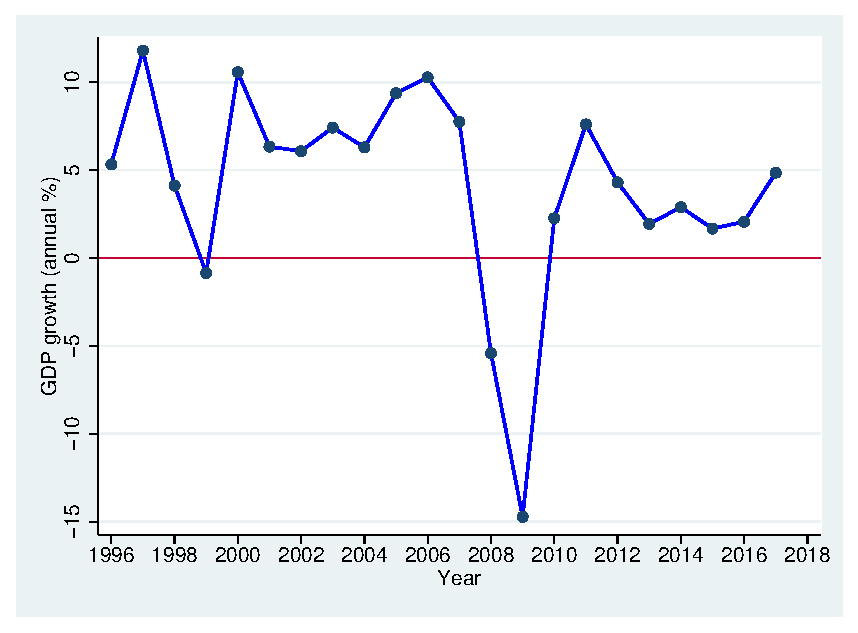
\includegraphics[width=0.6\linewidth]{Figure1.eps}
 \caption*{Source: World Bank - World Development Indicators}
\end{figure}

\DIFadd{The }\DIFaddend economic and political reforms \DIFdelbegin \DIFdel{, }\DIFdelend \DIFaddbegin \DIFadd{led to }\DIFaddend substantial
disparities in income and education opportunities
\DIFdelbegin \DIFdel{emerged
}\DIFdelend in the early 1990s \citep{Leping2008,
	lindemann+saar2011Russian2ndGeneration}. The inter-ethnic contacts
are largely limited to superficial encounters at work and in public
space, the \DIFaddbegin \DIFadd{number of }\DIFaddend close private ties remain limited
\citep{korts2009JofBaltStud}. \DIFdelbegin \DIFdel{Both ethnic groups have only few  are
largely living on their own with limited contacts. }\DIFdelend The
separate worlds are also reflected in media which may present quite
different and occasionally antagonistic viewpoints depending on the
language \citep{Korts2002}.
\DIFdelbegin \DIFdel{Around 25\% of Estonians show little
tolerance for Russian-speaking population (the corresponding figure
for Russians is substantially smaller).  A major issue for this group
is Russians' ability and willingness to communicate in Estonian.
}\DIFdelend 


\section{Data}
\label{subsec:ss_var}

\subsection{Variables and Sample Selection}
\label{sec:variables}

Our main analysis relies on the Estonian Labour Force Survey (ELFS),
first conducted in \DIFdelbegin \DIFdel{1995. }\DIFdelend \DIFaddbegin \DIFadd{1995 by the Estonian Statistical Office. We limit
ourselves with years 2000--2012 in the main analysis, motivated by a
methodology break: }\DIFaddend Until 1999 the survey was \DIFaddbegin \DIFadd{conducted as }\DIFaddend an annual
cross-section and later as a quarterly rotating panel. The \DIFdelbegin \DIFdel{number of distinct individuals is around 4000 annually. However,
due to the rotating structure}\DIFdelend \DIFaddbegin \DIFadd{survey
contains data on approximately 4000 distinct individuals annually}\DIFaddend ,
\DIFaddbegin \DIFadd{however, due to its rotating nature, }\DIFaddend we have \DIFdelbegin \DIFdel{about }\DIFdelend \DIFaddbegin \DIFadd{roughly }\DIFaddend 16,000 annual
observations \DIFdelbegin \DIFdel{.
The reader should keep in mind that while the pre-2000 waves include retrospective income, they do not include retrospective language skills. In this way, the results before
1995 are partly based on extrapolation, assuming individual language
skills did not vary before that date.  In the main }\DIFdelend \DIFaddbegin \DIFadd{for each year since 2000. For the long-term }\DIFaddend analysis, we
\DIFdelbegin \DIFdel{only
analyse the 2000--2012 time period but we also provide a long-term
picture that includes }\DIFdelend \DIFaddbegin \DIFadd{also use }\DIFaddend the earlier waves\DIFdelbegin \DIFdel{from 1989--1999. }\DIFdelend \DIFaddbegin \DIFadd{. These waves also include a retrospective
section that contains income up to several years back.
}

\DIFaddend We limit ourselves to men and women in the main working age, between 25 and
55 years old. Further, we only analyse
individuals who are either working or actively looking for a job.
\DIFdelbegin %DIFDELCMD < 

%DIFDELCMD < %%%
\DIFdelend The dataset allows us to control for standard personal
characteristics and human capital variables, such as age, education
and family status. \DIFdelbegin \DIFdel{The central variables in this study are the same
as in }%DIFDELCMD < \citep{Leping2008}%%%
\DIFdel{:
}\DIFdelend \DIFaddbegin \DIFadd{We discuss the most important variables below.
}\DIFaddend 

In all waves of the survey, respondents are asked about their
\DIFdelbegin \emph{\DIFdel{ethnic nationality}}%DIFAUXCMD
\DIFdelend \DIFaddbegin \DIFadd{``ethnic nationality''}\DIFaddend . Typically, individuals have a single ethnic
identity. The answers are coded as ``Estonian'' or
``non--Estonian''. As most of those who do not consider themselves
Estonian use Russian as their primary language, we refer to this group
as ``Russians''.                                  

The labour market outcomes \DIFdelbegin \DIFdel{include }\DIFdelend \DIFaddbegin \DIFadd{we analyse are income, the }\DIFaddend ``last salary on the main job'' and
labour force status (working, unemployed or inactive). 

The survey includes self-reported language skills on languages used at
home \DIFdelbegin \DIFdel{, }\DIFdelend and all other languages they understand. The respondents are
\DIFdelbegin \DIFdel{give }\DIFdelend \DIFaddbegin \DIFadd{given }\DIFaddend some guidance in assessing their skills, they can report either
no knowledge, understanding \DIFaddbegin \DIFadd{only, speaking but not writing}\DIFaddend , \DIFdelbegin \DIFdel{speaking, }\DIFdelend writing, or using the
language at home. We consolidate this information into a dummy \DIFaddbegin \DIFadd{variable}\DIFaddend , equal
to \DIFdelbegin \DIFdel{zero
for languages one cannot speak (but potentially understand) and
unity }\DIFdelend \DIFaddbegin \DIFadd{one }\DIFaddend if one speaks \DIFdelbegin \DIFdel{, speaks }\DIFdelend or writes, or uses that language at
home\DIFdelbegin \DIFdel{.
}\DIFdelend \DIFaddbegin \DIFadd{, and zero otherwise. Hence, we disregard passive understanding
only.
}\DIFaddend 

For further evidence on ethnic and gender segregation at \DIFdelbegin \DIFdel{workplace }\DIFdelend \DIFaddbegin \DIFadd{the workplace, }\DIFaddend we use data
from 2008 Integration Monitor Survey. The survey was conducted by
SaarPoll and focuses on
ethnic relations in Estonia. The sample size is 1500,
500 of the respondents consider themselves not ethnic Estonians. We analyse
two questions: ``which is the language of communication at your
workplace?'' and ``which languages do you need at work''. The first
question addresses the ethnic segregation while the second focuses on
the need \DIFdelbegin \DIFdel{of }\DIFdelend \DIFaddbegin \DIFadd{for }\DIFaddend communication.


\subsection{Descriptive Statistics}
\label{sec:descriptive}

The average wages, language skills and other explanatory variables together with the relative frequencies for the period 2000--2012 are presented in \cref{tab:descriptive}. We report the data separately for ethnic nationalities (Estonians and Russians) and language
skills (Estonian, Russian and English).

The table indicates that there are substantial disparities between
Estonians and Russians in wage and unemployment. For instance, the
average monthly salary\footnote{When interpreting \DIFdelbegin \DIFdel{the wage}\DIFdelend \DIFaddbegin \DIFadd{these figures}\DIFaddend ,
 one should keep in mind that during \DIFdelbegin \DIFdel{the }\DIFdelend \DIFaddbegin \DIFadd{this }\DIFaddend period\DIFdelbegin \DIFdel{of observation}\DIFdelend , 2000-2012, the average \DIFaddbegin \DIFadd{monthly }\DIFaddend salary \DIFdelbegin \DIFdel{increased }\DIFdelend \DIFaddbegin \DIFadd{grow }\DIFaddend by 180\%,
 from \EUR{314} to \EUR{887} \DIFdelbegin \DIFdel{monthly}\DIFdelend \DIFaddbegin \DIFadd{while the language knowledge changed rapidly as
well}\DIFaddend . \DIFdelbegin %DIFDELCMD < 

%DIFDELCMD < %%%
\DIFdelend \DIFaddbegin \DIFadd{However, the ethnic composition of the workforce remained roughly constant.}\DIFaddend } of Estonian
males who are not fluent in English is \EUR{532} while for Russians it
is only \EUR{452}. However, we also see that Russians who speak
English earn approximately 40\% more than those who do not (\EUR{452}
versus \EUR{326} monthly for men and \EUR{307} versus \EUR{221} for
women). Estonian skills are associated with lower income premium, 15\%
for men (\EUR{378} versus \EUR{329} monthly) and 30\% for women
(\EUR{260} versus \EUR{203}). \DIFdelbegin \DIFdel{Similarly, English is }\DIFdelend \DIFaddbegin \DIFadd{Analogously, English language skills are }\DIFaddend more closely
associated with income for Estonians \DIFdelbegin \DIFdel{than Russian language }\DIFdelend \DIFaddbegin \DIFadd{compared to Russian language skills}\DIFaddend . In
contrast, unemployment shows a different picture. For ethnic Russians,
it is Estonian language fluency that is more closely associated with
low unemployment, those fluent in Estonian have 11.2 percent
unemployment rate while for those not fluent it is 17.3 percent. The
corresponding numbers for English are 11.2 and 15.1. For Estonians,
English is more closely associated with unemployment than Russian:
Estonians fluent in English have \DIFdelbegin \DIFdel{in }\DIFdelend \DIFaddbegin \DIFadd{on }\DIFaddend average 5.0 percent unemployment
while those who are not fluent have 8.8 percent. The difference
related to Russian fluency is only 1.6 percentage points. However,
these \DIFdelbegin \DIFdel{associations }\DIFdelend \DIFaddbegin \DIFadd{correlations }\DIFaddend are not easy to interpret as \DIFaddbegin \DIFadd{besides of the strong
time trends, }\DIFaddend English skills are
also related to education, metropolitan residence, and general
ability.

% Table generated by Excel2LaTeX from sheet 'subgroups_by_ethnic_language'
\begin{sidewaystable}[htbp]
	\centering
	\caption{Averages and relative frequencies of selected explanatory
		variables 2000 -- 2012}
	\begin{tabular}{l|rrrr|rrrr}
		\toprule
		& \multicolumn{4}{c|}{Estonians}  &  \multicolumn{4}{c}{Russians}  \\ \midrule
		Variable          & RUS 0 & RUS 1 & ENG 0 & ENG 1 & EST 0 & EST 1 & ENG 0 & ENG 1 \\ \midrule
		Wage, men (EUR)       & 543.86 & 537.22 & 438.53 & 738.63 & 401.59 & 489.96 & 388.91 & 660.39 \\
		Wage, women (EUR)      & 345.51 & 376.98 & 301.13 & 488.83 & 238.25 & 338.62 & 266.87 & 435.60 \\
		Unemployment (\%)      & 8.74  & 7.13  & 8.83  & 4.99  & 17.30 & 11.18 & 15.06 & 11.23 \\
		EST 1 (\%)         & 99.97 & 99.58 & 99.50 & 99.95 & 0.00  & 100.00 & 40.84 & 80.97 \\
		RUS 1 (\%)         & 0.00  & 100.00 & 77.35 & 82.86 & 99.90 & 99.04 & 99.65 & 98.77 \\
		ENG 1 (\%)         & 29.47 & 37.16 & 0.00  & 100.00 & 6.70  & 30.69 & 0.00  & 100.00 \\
		College Degree (\%)     & 15.61 & 23.44 & 10.77 & 41.38 & 12.66 & 28.64 & 13.93 & 49.16 \\
		Married (\%)        & 40.09 & 55.71 & 54.11 & 49.53 & 63.54 & 60.78 & 63.38 & 56.99 \\
		Inter-ethnic household (\%) & 1.34  & 5.20  & 4.79  & 3.70  & 5.07  & 19.46 & 11.97 & 12.17 \\
		Age             & 37.05 & 41.83 & 42.39 & 38.05 & 42.14 & 40.54 & 42.15 & 37.83 \\
		Kids (number)        & 1.08  & 1.00  & 1.00  & 1.00  & 0.71  & 0.76  & 0.75  & 0.68  \\
		\textbf{Residence County } &    &    &    &    &    &    &    &    \\
		Metropolitan (\%)      & 17.74 & 22.58 & 14.03 & 35.25 & 35.43 & 56.37 & 38.82 & 75.50 \\
		North-East (\%)       & 0.64  & 3.14  & 3.46  & 1.10  & 53.84 & 15.85 & 40.90 & 11.54 \\
		\textbf{Workplace}     &    &    &    &    &    &    &    &    \\
		Tenure (years)       & 6.17  & 7.33  & 7.45  & 6.40  & 8.19  & 7.23  & 8.08  & 5.99  \\
		Public sector (\%)     & 20.03 & 24.81 & 21.79 & 27.55 & 11.62 & 21.67 & 16.28 & 18.14 \\
		Primary sector (\%)     & 14.10 & 9.80  & 13.00 & 6.43  & 9.91  & 7.46  & 8.82  & 8.11  \\
		Secondary sector (\%)    & 31.02 & 27.20 & 32.63 & 19.41 & 47.21 & 29.72 & 41.54 & 24.07 \\
		Tertiary sector (\%)    & 26.17 & 30.12 & 26.52 & 34.46 & 27.17 & 33.96 & 28.37 & 40.96 \\
		\# \DIFdelbegin \DIFdel{observations             }\DIFdelend \DIFaddbegin \DIFadd{Observations       }\DIFaddend & 14,943 & 57,270 & 46,525 & 25,688 & 13,805 & 12,830 & 21,773 & 4,862 \\ \bottomrule
	\end{tabular}%
	\label{tab:descriptive}%
                             \DIFdelbegin %DIFDELCMD < \caption*{\small
%DIFDELCMD < 		Workplace--related variables are reported for employed individuals,
%DIFDELCMD < 		other variables for the complete workforce.  Sample is limited to persons
%DIFDELCMD < 		25-55 year old.\\
%DIFDELCMD < 		\emph{RUS 0} refers to individuals who cannot speak Russian and
%DIFDELCMD < 		\emph{RUS 1} to those who can. Analogously for English and
%DIFDELCMD < 		Estonian.\\
%DIFDELCMD < 		Primary sector = Agriculture,
%DIFDELCMD < 		Fishing, Mining \\ Secondary sector = Manufacturing,
%DIFDELCMD < 		Construction, Electricity \\ Tertiary (service) sector =
%DIFDELCMD < 		Wholesale, Hotels, Transport, Financial intermediation, Real
%DIFDELCMD < 		estate \\ Public sector = Public administration, Education,
%DIFDELCMD < 		Health}
%DIFDELCMD < %%%
\DIFdelend \DIFaddbegin 

                           
	\caption*{\small
				Workplace--related variables are reported for employed individuals,
			other variables for the complete workforce. Sample is limited to persons
			25-55 year old.\\
			\emph{RUS 0} refers to individuals who do not speak Russian and
			\emph{RUS 1} to those who do. Analogously for  
			English
			(ENG) and
			Estonian (EST).\\
			Primary sector = Agriculture,
			Fishing, Mining \\ Secondary sector = Manufacturing,
			Construction, Electricity \\ Tertiary (service) sector =
			Wholesale, Hotels, Transport, Financial intermediation, Real
			estate \\ Public sector = Public administration, Education,
			Health
		}
\DIFaddend \end{sidewaystable}%

The language fluency variables clearly show that ethnic identity is
closely related to language use: more than 99\% of Estonians report
being fluent in Estonian, the figure for Russians is similar. We
also see that Estonians are better \DIFdelbegin \DIFdel{in }\DIFdelend \DIFaddbegin \DIFadd{at }\DIFaddend English than Russians and they
are also better \DIFdelbegin \DIFdel{in }\DIFdelend \DIFaddbegin \DIFadd{at }\DIFaddend Russian than vice versa.

Average age reflects the trend of younger generations
being more fluent in English and Estonian while older Estonians being
better in Russian. The family \DIFdelbegin \DIFdel{variables follow }\DIFdelend \DIFaddbegin \DIFadd{status--related variables correspond to }\DIFaddend the
respective age distribution. Not surprisingly, inter-ethnic
households include \DIFaddbegin \DIFadd{a }\DIFaddend disproportionally large share of Russian speaking
Estonians and Estonian speaking Russians.
The average experience follows the same pattern as age.
Public sector jobs are associated with disproportionally large share of
Estonian fluency among Russian workers, probably reflecting the formal
language requirements and little room for ethnic segregation in that
sector.

In conclusion, the descriptive analysis suggests that for Russians,
English skills are a more important driver for income than Estonian
skills while the opposite is true for unemployment. The labour market
outcomes of Estonians are substantially better correlated with English
skills than with Russian skills.



\section{Method}
\label{sec:method}

We analyse the relationship between labour market outcomes and language
skills \DIFdelbegin \DIFdel{by }\DIFdelend \DIFaddbegin \DIFadd{using the }\DIFaddend ordinary multivariate regression\DIFdelbegin \DIFdel{models}\DIFdelend .
Several related studies use instrumental variables to correct for
omitted variable bias and measurement errors \citep{Chiswick1995, bleakley+chin2004}.
%DIF < \ot{more examples here}
We refrain from doing that. Our decision is mainly \DIFdelbegin \DIFdel{data driven}\DIFdelend \DIFaddbegin \DIFadd{data-driven}\DIFaddend ,
there are no suitable instruments in our data,\footnote{We run an IV
	regression using \DIFdelbegin \DIFdel{age--at--immigration }\DIFdelend \DIFaddbegin \DIFadd{age at immigration }\DIFaddend to instrument Estonian skills
	for those Russians who were in the country at 1990. The results are
	not statistically significant at any conventional level.} but it also facilitates
comparison with other studies. For instance,
\citet{azam+2013EDandCC} and \citet{paolo+tansel2015JofDevStud} only
report OLS results\DIFdelbegin \DIFdel{.
}%DIFDELCMD < 

%DIFDELCMD < %%%
\DIFdel{There is also evidence from job language requirements suggesting that
the reduced-form evidence is not too different from the causal effect
}%DIFDELCMD < \citep{beblavy+2016CEPS}%%%
\DIFdel{.
}%DIFDELCMD < 

%DIFDELCMD < \citet{azam+2013EDandCC} %%%
\DIFdel{and}%DIFDELCMD < \citet{paolo+tansel2015JofDevStud}%%%
\DIFdel{, who use proxy variables to control for
individual ability, find these having }\DIFdelend \DIFaddbegin \DIFadd{, and, even more, find that the available proxy
variables have }\DIFaddend little influence on the \DIFdelbegin \DIFdel{effect
of language skills}\DIFdelend \DIFaddbegin \DIFadd{final results}\DIFaddend .

We \DIFdelbegin \DIFdel{estimate unemployment probability by linear probability model
}\DIFdelend \DIFaddbegin \DIFadd{use linear probability models }\DIFaddend (LPM) to \DIFaddbegin \DIFadd{estimate the relationship between
language skills and unemployment, mainly in order to }\DIFaddend avoid unnecessary parametric
assumptions in the corresponding binary choice models.\footnote{The
	results of corresponding probit models are virtually \DIFdelbegin \DIFdel{equal }\DIFdelend \DIFaddbegin \DIFadd{identical }\DIFaddend to the LPM results.}
Similarly, we estimate the effect of language skills on wage by
OLS. 
\DIFdelbegin \DIFdel{We correct the estimates for the panel data structure by
clustering the standard errors by individuals.
}\DIFdelend 

We \DIFdelbegin \DIFdel{estimate the basic model in the following form:
}\begin{displaymath}
	\DIFdel{%DIFDELCMD < \label{eq:specification}%%%
	\begin{split}
		y_{it} = &\: \alpha_{0} +
		\beta_{RUS} \cdot RUS_{it} +
		\beta_{EST} \cdot EST_{it} +
		\beta_{ENG} \cdot ENG_{it} +
		\\
		& + \vec{\beta}_{X}' \vec{X}_{it} +
		\upsilon_t + \epsilon_{it},
	\end{split}
}\end{displaymath}
%DIFAUXCMD
\DIFdel{where $y_{it}$ is the outcome (either unemployment indicator
or log-wage) }\DIFdelend \DIFaddbegin \DIFadd{describe the outcome (log wage and unemployment status) $y$ }\DIFaddend of individual $i$ \DIFdelbegin \DIFdel{in wave }\DIFdelend \DIFaddbegin \DIFadd{at year }\DIFaddend $t$ \DIFdelbegin \DIFdel{; $RUS$, $EST$, and $ENG$ are the }\DIFdelend \DIFaddbegin \DIFadd{as
}\begin{equation}
	\DIFadd{\label{eq:specification}
	\begin{split}                            
		y_{it} = &\: \vec{\alpha}' \vec{X}_{it} + \vec{\beta}{}' \vec{L}_{it} +
		\eta_{i} +
		\upsilon_{t} + \epsilon_{it},                                                                             
	\end{split}
}\end{equation}
\DIFadd{where $\vec{L}$ is the vector of
}\DIFaddend language skill descriptors\DIFdelbegin \DIFdel{; }\DIFdelend \DIFaddbegin \DIFadd{, }\DIFaddend $\vec{X}$ are the other individual
characteristics, \DIFaddbegin \DIFadd{$\eta_{i}$ is the individual-specific effect, }\DIFaddend $\upsilon_{t}$ are the year dummies and $\epsilon_{it}$
is the idiosyncratic error term. 
As we use panel data, we cluster the
standard errors on individuals. When analysing the \DIFaddbegin \DIFadd{long-term }\DIFaddend time
trend, we \DIFdelbegin \DIFdel{replace the main language effectsin~}%DIFDELCMD < \eqref{eq:specification} %%%
\DIFdel{by the
corresponding interactions
}\begin{eqnarray*}
	\DIFdel{\label{eq:time_interaction}
	\beta_{RUS,t} \cdot RUS_{it} \cdot \upsilon_{t} +
	\beta_{EST,t} \cdot EST_{it} \cdot \upsilon_{t} +
	\beta_{ENG,t} \cdot ENG_{it} \cdot \upsilon_{t}.
}\end{eqnarray*}
%DIFAUXCMD
\DIFdelend \DIFaddbegin \DIFadd{use the same specification (without year fixed effects) to
estimate separate models for each individual year.
}\DIFaddend 

We estimate three models that differ in \DIFdelbegin \DIFdel{terms of the number of
}\DIFdelend \DIFaddbegin \DIFadd{the }\DIFaddend control variables. The first \DIFdelbegin \DIFdel{one }\DIFdelend \DIFaddbegin \DIFadd{specification }\DIFaddend only includes the language skills
and year dummies. \DIFdelbegin \DIFdel{The second one also }\DIFdelend \DIFaddbegin \DIFadd{It describes the ``raw'' effect of language skills,
net of strong time trends in our data.
The second specification additionally }\DIFaddend includes individual
characteristics \DIFdelbegin \DIFdel{, such as }\DIFdelend \DIFaddbegin \DIFadd{(}\DIFaddend age, education\DIFdelbegin \DIFdel{, }\DIFdelend \DIFaddbegin \DIFadd{) and family descriptors (marital
status, an indicator for inter-ethnic marriage, having kids up to 17 years
old) }\DIFaddend and county of residence. 
Finally, the third \DIFdelbegin \DIFdel{model also includes }\DIFdelend \DIFaddbegin \DIFadd{specification also adds }\DIFaddend industry, occupation, and other
workplace descriptors.
\DIFaddbegin \DIFadd{Note that for the unemployment probability,
we only estimate the first two models.
}\DIFaddend 


\section{Results}
\label{sec:results}
\subsection{Unemployment}
\label{subsec:basic_model_unemployment}

The central results for unemployment regressions are \DIFdelbegin \DIFdel{given in
\mbox{%DIFAUXCMD
\cref{tab:unemployment_estimation_by_sex_and_ethnic}}\hspace{0pt}%DIFAUXCMD
.
}%DIFDELCMD < 

%DIFDELCMD < %%%
\DIFdelend \DIFaddbegin \DIFadd{presented in
\mbox{%DIFAUXCMD
\cref{tab:unemployment_estimation_by_sex_and_ethnic_same_sample}}\hspace{0pt}%DIFAUXCMD
}\footnote{\DIFadd{We
 restrict both models to have the same number of observations as
 requested by a reviewer. The unrestricted results are provided in the Appendix (\mbox{%DIFAUXCMD
\Cref{tab:unemployment_estimation_by_sex_and_ethnic}}\hspace{0pt}%DIFAUXCMD
).}}\DIFadd{.
}\DIFaddend The
table clearly indicates that Estonian language skills are associated
with approximately 5 percentage points lower unemployment for both
Russian men and women. We also see that the effect is not 
\DIFdelbegin \DIFdel{radically
influenced }\DIFdelend \DIFaddbegin \DIFadd{influenced in any major way }\DIFaddend by the individual characteristics--for men it is
virtually unchanged while for women the estimate falls by 30\%\DIFaddbegin \DIFadd{, from
6.5 to 4.5 percentage points}\DIFaddend .

\DIFdelbegin %DIFDELCMD < \begin{table}[t!]
%DIFDELCMD < 	\begin{center}
%DIFDELCMD < 		\caption{Estimation results for unemployment.}
%DIFDELCMD < 		\label{tab:unemployment_estimation_by_sex_and_ethnic}
%DIFDELCMD < 		\begin{tabular}{l D{.}{.}{3} @{\qquad} D{.}{.}{3} @{\qquad\qquad}
%DIFDELCMD < 				D{.}{.}{3} @{\qquad} D{.}{.}{3}}
%DIFDELCMD < 			\toprule
%DIFDELCMD < 			&         \multicolumn{2}{c}{Men}         &        \multicolumn{2}{c}{Women}        \\
%DIFDELCMD < 			Estonians:      & \multicolumn{1}{c}{1}      & \multicolumn{1}{l}{\hspace{10pt}2} & \multicolumn{1}{c}{1}      & \multicolumn{1}{c}{2}      \\
%DIFDELCMD < 			Russian         & -0.026^{***}               & -0.010                             & -0.009^{*}                 & 0.010^{**}                 \\
%DIFDELCMD < 			                & (0.006)                    & (0.006)                            & (0.005)                    & (0.005)                    \\
%DIFDELCMD < 			English         & -0.047^{***}               & -0.019^{***}                       & -0.024^{***}               & -0.008^{*}                 \\
%DIFDELCMD < 			                & (0.004)                    & (0.005)                            & (0.004)                    & (0.004)                    \\
%DIFDELCMD < 			\# obs          & \multicolumn{1}{c}{36,160} & \multicolumn{1}{l}{36,132}         & \multicolumn{1}{l}{36,050} & \multicolumn{1}{c}{36,015} \\
%DIFDELCMD < 			$R^{2}$         & 0.022                      & 0.047                              & 0.012                      & 0.036                      \\ \hline
%DIFDELCMD < 			Russians: & \\
%DIFDELCMD < 			Estonian        & -0.052^{***}               & -0.052^{***}                       & -0.065^{***}               & -0.045^{***}               \\
%DIFDELCMD < 			                & (0.010)                    & (0.011)                            & (0.009)                    & (0.010)                    \\
%DIFDELCMD < 			English         & -0.020                     & 0.006                              & -0.015                     & -0.003                     \\
%DIFDELCMD < 			                & (0.012)                    & (0.014)                            & (0.011)                    & (0.012)                    \\
%DIFDELCMD < 			\# obs          & \multicolumn{1}{c}{12,946} & \multicolumn{1}{l}{12,942}         & \multicolumn{1}{l}{13,689} & \multicolumn{1}{c}{13,674} \\
%DIFDELCMD < 			$R^{2}$         & 0.033                      & 0.066                              & 0.023                      & 0.043                      \\ \hline
%DIFDELCMD < 			year dummies    & \V                         & \V                                 & \V                         & \V                         \\
%DIFDELCMD < 			indiv. charact. &                            & \V                                 &                            & \V                         \\
%DIFDELCMD < 			\bottomrule
%DIFDELCMD < 		\end{tabular}%
%DIFDELCMD < 		\begin{flushleft}
%DIFDELCMD < 			\caption*{ \legend \\ Standard errors (clustered on individuals) in parentheses.}
%DIFDELCMD < 		\end{flushleft}
%DIFDELCMD < 	\end{center}
%DIFDELCMD < 

%DIFDELCMD < \end{table}%%%

\DIFdelend \DIFaddbegin \begin{table}[h]
	\begin{center}
		\textcolor{Blue}{
		\caption{Estimation results for unemployment.}
		\label{tab:unemployment_estimation_by_sex_and_ethnic_same_sample} %SKB 04.07.2018 14:22:Not yet updated only prepared
		\begin{tabular}{l D{.}{.}{3} @{\qquad} D{.}{.}{3} @{\qquad\qquad}
				D{.}{.}{3} @{\qquad} D{.}{.}{3}}
			\toprule
			&     \multicolumn{2}{c}{Men}     &    \multicolumn{2}{c}{Women}    \\
			Estonians:   & \multicolumn{1}{c}{1}   & \multicolumn{1}{l}{\hspace{10pt}2} & \multicolumn{1}{c}{1}   & \multicolumn{1}{c}{2}   \\ \midrule
			Russian     & -0.026^{***}        & -0.001               & -0.009^{*}         & 0.010^{**}         \\
			        & (0.006)          & (0.006)              & (0.005)          & (0.005)          \\
			English     & -0.047^{***}        & -0.019^{***}            & -0.024^{***}        & -0.008^{*}         \\
			        & (0.004)          & (0.005)              & (0.004)          & (0.004)          \\
			\# Observations     & \multicolumn{1}{c}{36,132} & \multicolumn{1}{l}{36,132}     & \multicolumn{1}{l}{36,015} & \multicolumn{1}{c}{36,015} \\
			$R^{2}$     & 0.022           & 0.047               & 0.012           & 0.036           \\ \hline
			Russians: & \\
			Estonian    & -0.052^{***}        & -0.052^{***}            & -0.065^{***}        & -0.045^{***}        \\
			        & (0.010)          & (0.011)              & (0.009)          & (0.010)          \\
			English     & -0.020          & 0.006               & -0.014           & -0.003           \\
			        & (0.012)          & (0.014)              & (0.011)          & (0.012)          \\
			\# Observations     & \multicolumn{1}{c}{12,942} & \multicolumn{1}{l}{12,942}     & \multicolumn{1}{l}{13,674} & \multicolumn{1}{c}{13,674} \\
			$R^{2}$     & 0.033           & 0.066               & 0.023           & 0.043           \\ \hline
			year dummies  & \V             & \V                 & \V             & \V             \\
			indiv. charact. &              & \V                 &              & \V             \\
			\bottomrule
		\end{tabular}
		\begin{flushleft}
			\caption*{ \legend \\ Standard errors (clustered on individuals) in parentheses; \\  Individual characteristics are \modelTwo.  \restrictions }
		\end{flushleft}
	}
	\end{center}
\end{table}\DIFaddend %

Neither Russian nor English show a comparably strong effect.
Knowledge of Russian is not associated with less unemployment for
Estonian men, and is even related to a slightly higher unemployment
for Estonian women. The latter outcome may be related to omitted
variable bias, Russian knowledge was widespread \DIFdelbegin \DIFdel{before 1990 }\DIFdelend \DIFaddbegin \DIFadd{in the Soviet era }\DIFaddend and may
not have been closely associated with \DIFdelbegin \DIFdel{any favourable characteristics,
but during the period was increasingly more }\DIFdelend \DIFaddbegin \DIFadd{favourable unobserved
characteristics, however, it has been increasingly }\DIFaddend associated with age
\DIFaddbegin \DIFadd{through the period of analysis}\DIFaddend .
English skills are related to less unemployment both for Estonian men
and women, but the effect is small.
For Russians, \DIFdelbegin \DIFdel{however, Estonian language skills matter}\DIFdelend \DIFaddbegin \DIFadd{the most important language is clearly Estonian}\DIFaddend . Those who are
fluent in that language \DIFdelbegin \DIFdel{have }\DIFdelend \DIFaddbegin \DIFadd{are }\DIFaddend approximately 5 percentage point less \DIFdelbegin \DIFdel{unemployment}\DIFdelend \DIFaddbegin \DIFadd{likely
unemployed}\DIFaddend , the effect changes only a little when \DIFdelbegin \DIFdel{controlling for
individual characteristics}\DIFdelend \DIFaddbegin \DIFadd{introducing the
individual controls}\DIFaddend . In contrast, the effect of English
\DIFdelbegin \DIFdel{fluency }\DIFdelend is close to zero and not statistically significant. As in \DIFaddbegin \DIFadd{the
}\DIFaddend case of Estonian, individual characteristics change the estimates only
a little.

In summary, these results suggest that \DIFdelbegin \DIFdel{the Estonian language is important for }\DIFdelend \DIFaddbegin \DIFadd{Estonian is the only language
that matters for the }\DIFaddend employment prospects. \DIFdelbegin \DIFdel{The role of English is
small, and that of
Russian is almost non-existent despite a largely
bilingual service sector in the country}\DIFdelend \DIFaddbegin \DIFadd{Despite widespread
bilingualism in the service sector, and increasing global importance of
English, these languages are not closely associated with unemployment
probability}\DIFaddend . 

\subsection{Wage\DIFdelbegin \DIFdel{Regressions}\DIFdelend }
%DIF > SKB: Adding occupation to Model 3 reduces the effects drastically. Beforehand I somehow forgot to add it to the estimation. Now occupation is included as it should have been in the first place.
\label{subsec:basic_model_wage}

\DIFdelbegin \DIFdel{\mbox{%DIFAUXCMD
\cref{tab:wage_estimation_by_sex_and_ethnic} }\hspace{0pt}%DIFAUXCMD
presents the
main
results.}%DIFDELCMD < 

%DIFDELCMD < %%%
\DIFdelend \DIFaddbegin \DIFadd{\mbox{%DIFAUXCMD
\cref{tab:wage_estimation_by_sex_and_ethnic_same_sample} }\hspace{0pt}%DIFAUXCMD
presents the
central wage regression
results.}\footnote{\DIFadd{As above, we
restrict both models to have the same number of observations as
requested by a reviewer. The unrestricted table is in the appendix \mbox{%DIFAUXCMD
\cref{tab:wage_estimation_by_sex_and_ethnic}}\hspace{0pt}%DIFAUXCMD
.}}
\DIFaddend The table
confirms \DIFaddbegin \DIFadd{the descriptive evidence }\DIFaddend that wage is positively associated
with fluency in \DIFdelbegin \DIFdel{other
languages , in particular English }\DIFdelend \DIFaddbegin \DIFadd{all analysed languages with English showing the
largest effect}\DIFaddend . The only \DIFdelbegin \DIFdel{remarkable }\DIFdelend exception is
Estonian language for Russian men where we fail to find any positive
effect for any \DIFdelbegin \DIFdel{model. This }\DIFdelend \DIFaddbegin \DIFadd{of the specifications. This finding }\DIFaddend qualitatively repeats the results of
\citet{Toomet2011}. However, for women we observe a sizeable
positive effect between \DIFdelbegin \DIFdel{12 }\DIFdelend \DIFaddbegin \DIFadd{6 }\DIFaddend and 16 percentage points, suggesting that
\citet{Toomet2011} results \DIFdelbegin \DIFdel{only describe the male }\DIFdelend \DIFaddbegin \DIFadd{are not valid for the female }\DIFaddend labour market. The effect decreases somewhat
(from 0.167 to 0.114) when including the individual characteristics
into the model, suggesting that the premium
is partly caused by education and potentially also by unobserved
individual performance. \DIFdelbegin \DIFdel{Observable workplace characteristics
do not
influence the estimates}\DIFdelend \DIFaddbegin \DIFadd{Adding observable workplace characteristics
lowers the effects further to 0.066, suggesting that part of the
language skill premium is realized through workplace selection}\DIFaddend .

\DIFdelbegin %DIFDELCMD < \begin{table}[htbp]
%DIFDELCMD < 	\begin{center}
%DIFDELCMD < 		\caption{Estimation results for log wage}
%DIFDELCMD < 		\label{tab:wage_estimation_by_sex_and_ethnic}
%DIFDELCMD < 		\begin{tabular}{l | D{.}{.}{3} @{\qquad} D{.}{.}{3} @{\qquad} D{.}{.}{3}  @{\qquad} | @{\qquad}
%DIFDELCMD < 				D{.}{.}{3} @{\qquad} D{.}{.}{3} @{\qquad} D{.}{.}{3}}
%DIFDELCMD < 			\toprule
%DIFDELCMD < 			&                                   \multicolumn{3}{c}{Men}                                    &                              \multicolumn{3}{c}{Women}                               \\
%DIFDELCMD < 			Estonians          & \multicolumn{1}{c}{1}      & \multicolumn{1}{c}{2}      & \multicolumn{1}{l}{\hspace{10pt}3} & \multicolumn{1}{c}{1}      & \multicolumn{1}{c}{2}      & \multicolumn{1}{c}{3}      \\\midrule
%DIFDELCMD < 			Russian            & 0.107^{***}                & 0.072^{***}                & 0.054^{***}                        & 0.096^{***}                & 0.041^{***}                & 0.035^{***}                \\
%DIFDELCMD < 			                   & (0.015)                    & (0.015)                    & (0.014)                            & (0.011)                    & (0.011)                    & (0.010)                    \\
%DIFDELCMD < 			English            & 0.343^{***}                & 0.162^{***}                & 0.145^{***}                        & 0.311^{***}                & 0.131^{***}                & 0.123^{***}                \\
%DIFDELCMD < 			                   & (0.013)                    & (0.015)                    & (0.013)                            & (0.010)                    & (0.010)                    & (0.010)                    \\
%DIFDELCMD < 			\# obs             & \multicolumn{1}{l}{22,290} & \multicolumn{1}{l}{21,785} & \multicolumn{1}{l}{22,274}         & \multicolumn{1}{l}{26,673} & \multicolumn{1}{l}{26,449} & \multicolumn{1}{c}{26,644} \\
%DIFDELCMD < 			$R^{2}$            & 0.726                      & 0.755                      & 0.790                              & 0.769                      & 0.810                      & 0.830                      \\ \midrule
%DIFDELCMD < 			Russians:          &  \\
%DIFDELCMD < 			Estonian           & 0.018                      & -0.014                     & 0.008                              & 0.167^{***}                & 0.114^{***}                & 0.125^{***}                \\
%DIFDELCMD < 			                   & (0.018)                    & (0.019)                    & (0.018)                            & (0.014)                    & (0.014)                    & (0.014)                    \\
%DIFDELCMD < 			English            & 0.249^{***}                & 0.155^{***}                & 0.137^{***}                        & 0.223^{***}                & 0.089^{***}                & 0.089^{***}                \\
%DIFDELCMD < 			                   & (0.026)                    & (0.027)                    & (0.026)                            & (0.021)                    & (0.022)                    & (0.020)                    \\
%DIFDELCMD < 			\# obs             & \multicolumn{1}{l}{8234}   & \multicolumn{1}{l}{7978}   & \multicolumn{1}{l}{8233}           & \multicolumn{1}{l}{9904}   & \multicolumn{1}{l}{9697}   & \multicolumn{1}{c}{9895}   \\
%DIFDELCMD < 			$R^{2}$            & 0.731                      & 0.746                      & 0.783                              & 0.794                      & 0.809                      & 0.837                      \\ \hline
%DIFDELCMD < 			year dummies       & \V                         & \V                         & \V                                 & \V                         & \V                         & \V                         \\
%DIFDELCMD < 			indiv. charact.    &                            & \V                         & \V                                 &                            & \V                         & \V                         \\
%DIFDELCMD < 			workplace charact. &                            &                            & \V                                 &                            &                            & \V                         \\ \bottomrule
%DIFDELCMD < 		\end{tabular}
%DIFDELCMD < 		\begin{flushleft}
%DIFDELCMD < 			\caption*{\legend \\ Standard errors (clustered on individuals) in parenthesis}
%DIFDELCMD < 		\end{flushleft}
%DIFDELCMD < 	\end{center}
%DIFDELCMD < \end{table}
%DIFDELCMD < %%%
\DIFdelend \DIFaddbegin \begin{table}[htbp]
	\begin{center}
		\textcolor{Blue}{
		\caption{Estimation results for log wage}
		\label{tab:wage_estimation_by_sex_and_ethnic_same_sample} %SKB 04.07.2018 14:22:Not yet updated only prepared
		%Accounting for occupation in model reduced the Estonian coefficient for women drastically (from 0.12 down 0.06)!
		%For other groups it is less
		\begin{tabular}{l | D{.}{.}{3} @{\qquad} D{.}{.}{3} @{\qquad} D{.}{.}{3} @{\qquad} | @{\qquad}
				D{.}{.}{3} @{\qquad} D{.}{.}{3} @{\qquad} D{.}{.}{3}}
			\toprule
			&                  \multicolumn{3}{c}{Men}                  &               \multicolumn{3}{c}{Women}                \\
			Estonians     & \multicolumn{1}{c}{\hspace{-12pt}1}   & \multicolumn{1}{l}{\hspace{12pt}2}   & \multicolumn{1}{l}{\hspace{12pt}3} & \multicolumn{1}{c}{\hspace{-12pt}1}   & \multicolumn{1}{l}{\hspace{12pt}2}   & \multicolumn{1}{c}{3}   \\\midrule
			Russian      & 0.112^{***}        & 0.078^{***}        & 0.043^{***}            & 0.094^{***}        & 0.039^{***}        & 0.016^{*}        \\
			          & (0.015)          & (0.015)          & (0.014)              & (0.011)          & (0.011)          & (0.009)          \\
			English      & 0.343^{***}        & 0.158^{***}        & 0.108^{***}            & 0.311^{***}        & 0.130^{***}        & 0.075^{***}        \\
			          & (0.013)          & (0.015)          & (0.013)              & (0.010)          & (0.010)          & (0.009)          \\
			\# Observations       & \multicolumn{1}{l}{21,785} & \multicolumn{1}{l}{21,785} & \multicolumn{1}{l}{21,785}     & \multicolumn{1}{l}{26,673} & \multicolumn{1}{l}{26,644} & \multicolumn{1}{c}{26,449} \\
			$R^{2}$      & 0.730           & 0.760           & 0.801               & 0.769           & 0.810           & 0.830           \\ \midrule
			Russians:     & \\
			Estonian      & 0.020           & -0.013           & -0.009               & 0.167^{***}        & 0.114^{***}        & 0.066^{***}        \\
			          & (0.018)          & (0.019)          & (0.018)              & (0.014)          & (0.014)          & (0.013)          \\
			English      & 0.248^{***}        & 0.152^{***}        & 0.103^{***}            & 0.223^{***}        & 0.089^{***}        & 0.054^{***}        \\
			          & (0.026)          & (0.027)          & (0.024)              & (0.021)          & (0.022)          & (0.018)          \\
			\# Observations       & \multicolumn{1}{l}{7978}  & \multicolumn{1}{l}{7978}  & \multicolumn{1}{l}{7978}      & \multicolumn{1}{l}{9904}  & \multicolumn{1}{l}{9895}  & \multicolumn{1}{c}{9697}  \\
			$R^{2}$      & 0.731           & 0.746           & 0.794               & 0.794           & 0.809           & 0.854           \\ \hline
			year dummies    & \V             & \V             & \V                 & \V             & \V             & \V             \\
			indiv. charact.  &              & \V             & \V                 &              & \V             & \V             \\
			workplace charact. &              &              & \V                 &              &              & \V             \\ \bottomrule
		\end{tabular}
		\begin{flushleft}
			\caption*{\legend \\ Standard errors (clustered on individuals) in parenthesis; \\ Individual characteristics are \modelTwo.  Workplace characteristics are \modelThreeAdd.  \restrictions}
		\end{flushleft}
	}
	\end{center}
\end{table}
\DIFaddend 

We also see that knowledge of Russian language is associated with a
substantial income premium of 10\% for both Estonian men and women.
\DIFdelbegin \DIFdel{The effect approximately halves when introducing
individual controls , suggesting that it is partly related to
education and potentially also to ability . It
falls further when also controlling for the
workplace characteristics, indicating that Estonians' income is
better characterized by available workplace
variables}\DIFdelend \DIFaddbegin \DIFadd{Individual and workplace controls lower this figure substantially
implying that both, ability bias
and workplace mobility, play a role}\DIFaddend .

English language \DIFaddbegin \DIFadd{fluency }\DIFaddend is associated with a very large
wage premium, up to 34 log points\DIFdelbegin \DIFdel{(model 1 for Estonian men). It }\DIFdelend \DIFaddbegin \DIFadd{, for all the analysed groups. The number }\DIFaddend falls substantially when introducing the
individual characteristics into the model (model 2), additional
workplace characteristics have \DIFdelbegin \DIFdel{little }\DIFdelend \DIFaddbegin \DIFadd{less }\DIFaddend effect. However, in all specifications it \DIFdelbegin \DIFdel{is
significantly }\DIFdelend \DIFaddbegin \DIFadd{remains noticeably }\DIFaddend more
important than Russian for Estonians \DIFaddbegin \DIFadd{in all
specifications}\DIFaddend . The estimates are rather
similar for Estonian and Russian men but little lower for Russian
women than for Estonian women.

In conclusion, the wage regressions suggest that English is the
\DIFdelbegin \DIFdel{main
language that matters }\DIFdelend \DIFaddbegin \DIFadd{language which is most closely associated with income }\DIFaddend for men. The effect of Russian \DIFaddbegin \DIFadd{language fluency }\DIFaddend is minor and
that of Estonian \DIFaddbegin \DIFadd{language fluency }\DIFaddend non-existent. For women, all three languages are
associated with higher wage but \DIFdelbegin \DIFdel{Russian }\DIFdelend \DIFaddbegin \DIFadd{the Russian language }\DIFaddend to a smaller extent.
This \DIFaddbegin \DIFadd{result }\DIFaddend is in a stark contrast to the unemployment regressions \DIFdelbegin \DIFdel{, }\DIFdelend \DIFaddbegin \DIFadd{and }\DIFaddend we return to
this question in the discussion \DIFaddbegin \DIFadd{below}\DIFaddend .


\section{Extensions}
\label{sec:extensions}

\subsection{A Long-Run View}
\label{sec:long-run}              

\DIFaddbegin \DIFadd{As the Estonian economy went through turbulent times and rapid changes
during the 1990s, it is instructive to analyse the effect long-term
trends in the estimated effect size. }\DIFaddend Here we look at the yearly estimates from 1992 to 2012.
\DIFdelbegin \DIFdel{We report those for the model 2.}\DIFdelend \DIFaddbegin \DIFadd{The reader should keep in mind that while the pre-2000 waves include retrospective income, they do not include retrospective language skills. In this way, the results before
1995 are partly based on extrapolation, assuming an individual's language
skills did not vary before that date.
}

\DIFadd{We report the results for model 2, i.e. models that include year
dummies and individual controls, but not workplace
characteristics.}\DIFaddend \footnote{The results for \DIFdelbegin \DIFdel{other }\DIFdelend models \DIFaddbegin \DIFadd{with workplace data (model
 3 for wage)
 }\DIFaddend look \DIFdelbegin \DIFdel{essentially the same}\DIFdelend \DIFaddbegin \DIFadd{qualitatively similar}\DIFaddend . \DIFdelbegin \DIFdel{If we add more variables like }\DIFdelend \DIFaddbegin \DIFadd{More controls }\DIFaddend in \DIFaddbegin \DIFadd{the }\DIFaddend model \DIFdelbegin \DIFdel{3 then }\DIFdelend \DIFaddbegin \DIFadd{reduce }\DIFaddend the effect size \DIFdelbegin \DIFdel{reduces by about five to ten percentage points, }\DIFdelend but \DIFdelbegin \DIFdel{the overall picture remains the same}\DIFdelend \DIFaddbegin \DIFadd{does not qualitatively
 change its temporal pattern}\DIFaddend .}

The effect \DIFdelbegin \DIFdel{on }\DIFdelend \DIFaddbegin \DIFadd{of }\DIFaddend language fluency on unemployment is shown on
Figure~\ref{fig:long-run_unemployment}\DIFaddbegin \DIFadd{, }\DIFaddend and on wage on
Figure~\ref{fig:long-run_wage}\DIFdelbegin %DIFDELCMD < 

%DIFDELCMD < \begin{figure}[hbtp]
%DIFDELCMD < 	\centering
%DIFDELCMD < 	\subfigure[Non-native languages for men]{
%DIFDELCMD < 		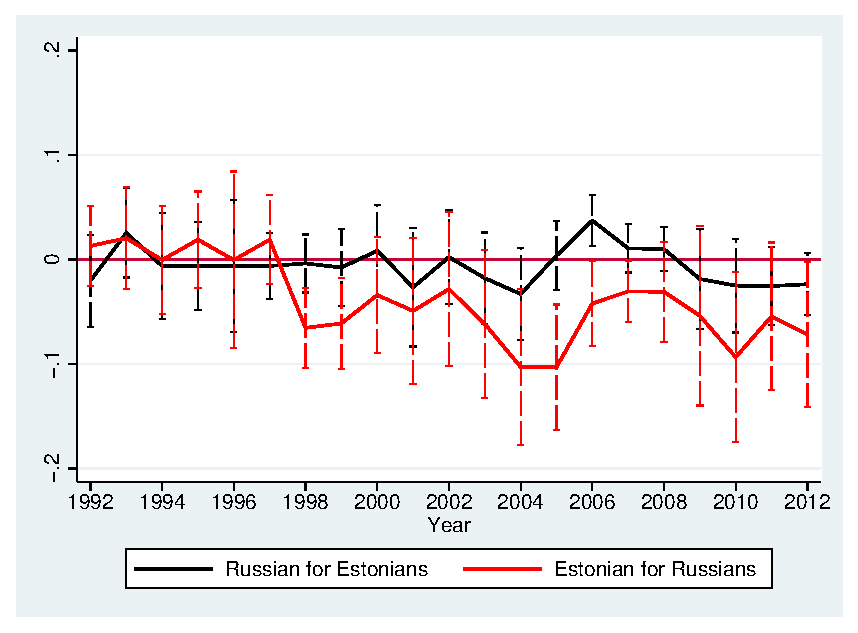
\includegraphics[width=0.45\linewidth]{Figure1a.eps}
%DIFDELCMD < 

%DIFDELCMD < 		\label{fig:long-run_unemployment_estonian_russian_men}
%DIFDELCMD < 	}
%DIFDELCMD < 	\subfigure[Non-native languages for women]{
%DIFDELCMD < 		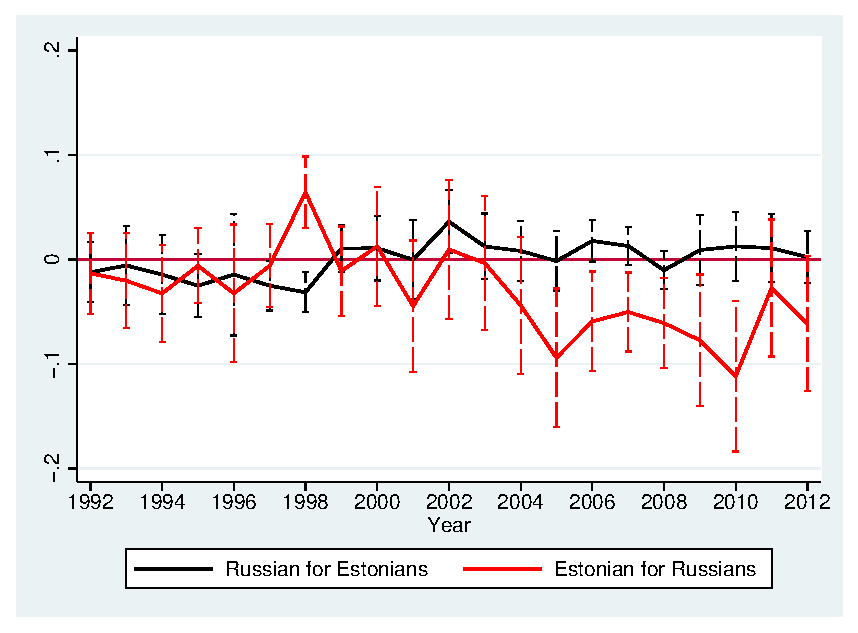
\includegraphics[width=0.45\linewidth]{Figure1b.eps}
%DIFDELCMD < 		\label{fig:long-run_unemployment_estonian_russian_women}
%DIFDELCMD < 	}
%DIFDELCMD < 	\subfigure[English for Men]{
%DIFDELCMD < 		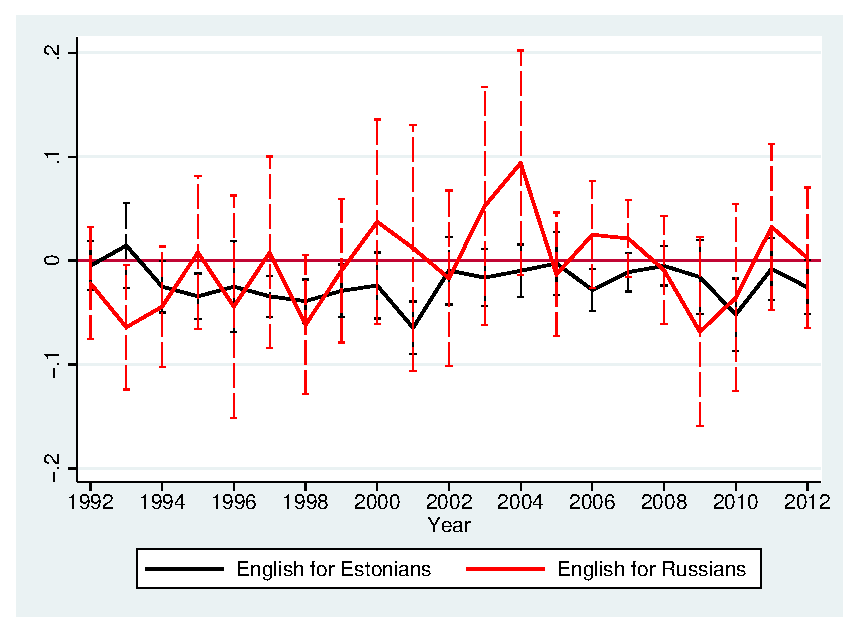
\includegraphics[width=0.45\linewidth]{Figure1c.eps}
%DIFDELCMD < 		\label{fig:long-run_unemployment_english_men}
%DIFDELCMD < 	}
%DIFDELCMD < 	\subfigure[English for Women]{
%DIFDELCMD < 		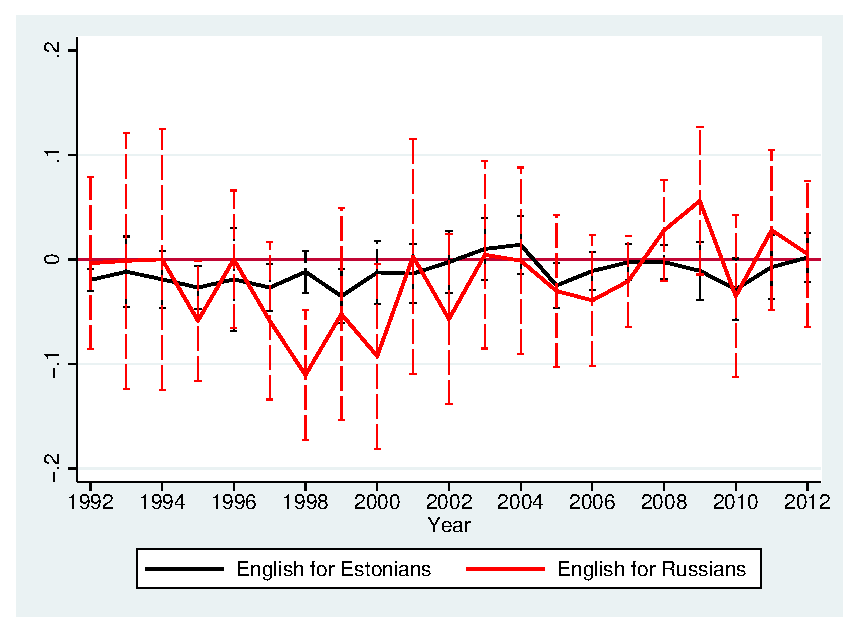
\includegraphics[width=0.45\linewidth]{Figure1d.eps}
%DIFDELCMD < 		\label{fig:long-run_unemployment_english_women}
%DIFDELCMD < 	}
%DIFDELCMD < 	%%%
%DIFDELCMD < \caption{%
{%DIFAUXCMD
\DIFdelFL{The effect of language fluency on unemployment, 1992--2012}}
	%DIFAUXCMD
%DIFDELCMD < \label{fig:long-run_unemployment}
%DIFDELCMD < \end{figure}
%DIFDELCMD < 

%DIFDELCMD < %%%
\DIFdelend \DIFaddbegin \DIFadd{.
}\DIFaddend The results reveal a few interesting facts. First, the effects are
relatively stable over time, indicating that neither economic
environment nor the data quality have changed rapidly. Estonian
fluency has been associated with less unemployment for both \DIFaddbegin \DIFadd{Russian }\DIFaddend men and
women since around \DIFaddbegin \DIFadd{the }\DIFaddend year 2000, in \DIFaddbegin \DIFadd{the }\DIFaddend 1990s it had little effect. Russian fluency,
in contrast, had never \DIFaddbegin \DIFadd{had }\DIFaddend an impact on \DIFaddbegin \DIFadd{Estonians' }\DIFaddend unemployment probability.

\DIFaddbegin \begin{figure}[hbt]
	\centering
	\subfigure[Non-native languages for men]{
		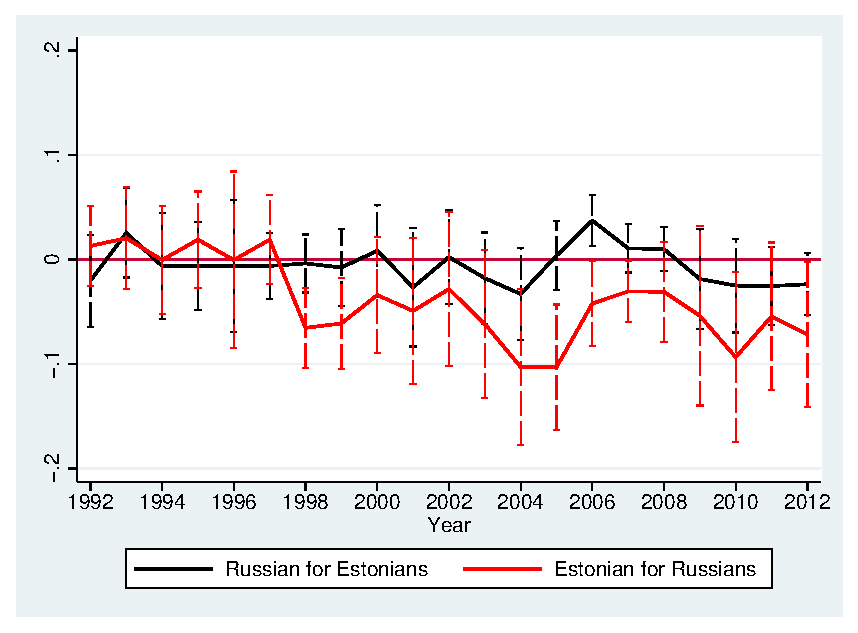
\includegraphics[width=0.45\linewidth]{Figure2a.eps}

		\label{fig:long-run_unemployment_estonian_russian_men}
	}
	\subfigure[Non-native languages for women]{      
		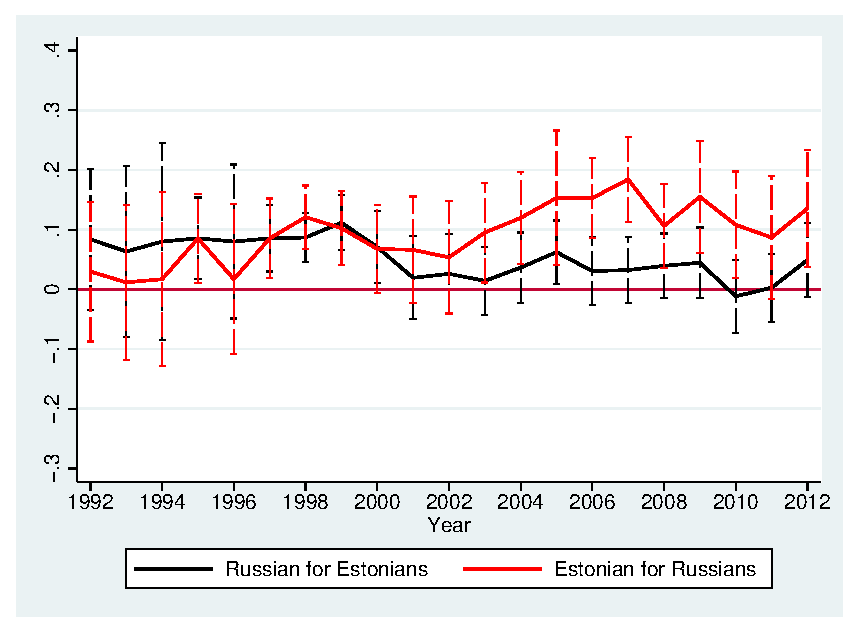
\includegraphics[width=0.45\linewidth]{Figure2b.eps}
		\label{fig:long-run_unemployment_estonian_russian_women}
	}
	\subfigure[English for Men]{
		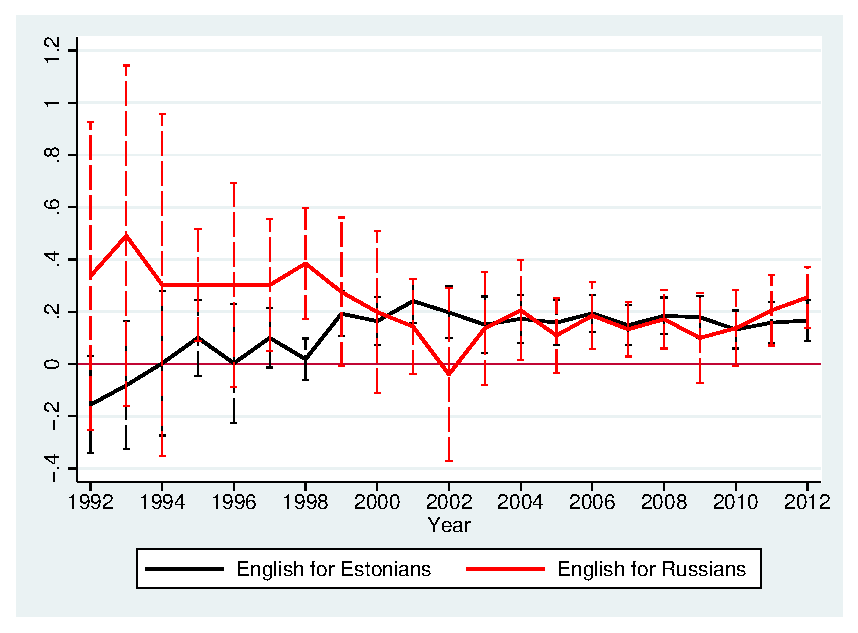
\includegraphics[width=0.45\linewidth]{Figure2c.eps}
		\label{fig:long-run_unemployment_english_men}
	}
	\subfigure[English for Women]{
		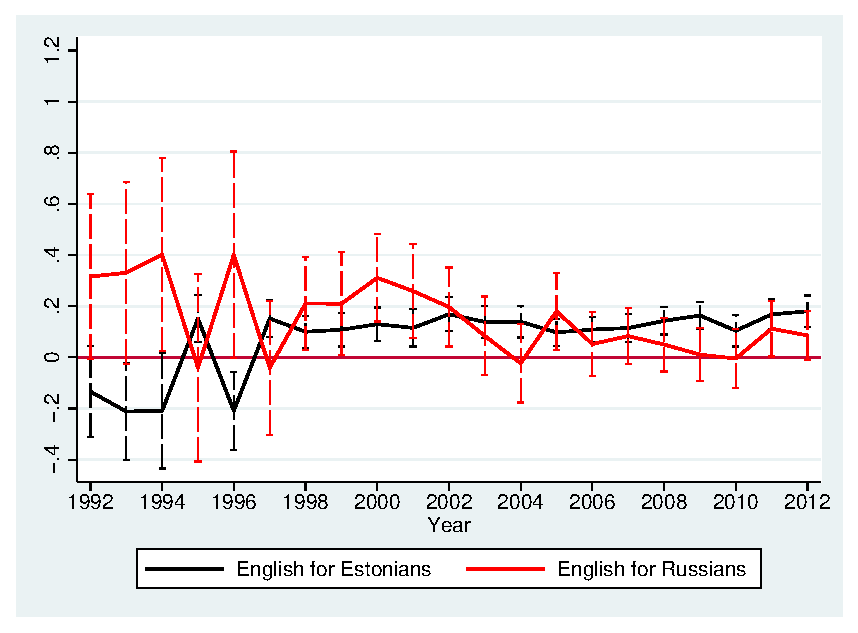
\includegraphics[width=0.45\linewidth]{Figure2d.eps}
		\label{fig:long-run_unemployment_english_women}
	}
	\caption{\DIFaddFL{The effect of language fluency on unemployment, 1992--2012. }\\ \DIFaddFL{Control variables are \modelTwo. \agerestrictions }}
	\label{fig:long-run_unemployment}
\end{figure}

\DIFaddend For Estonian men, fluency in English is associated with less unemployment through the whole
period of observation whereas fluency in Russian has no effect.
Only \DIFaddbegin \DIFadd{a }\DIFaddend few of the results are \DIFdelbegin \DIFdel{statistically significant pointwise }\DIFdelend \DIFaddbegin \DIFadd{point wise statistically significant }\DIFaddend though.
For Estonian women, both languages are associated with less
unemployment in the 1990s but not later. The picture is different for
Russians. For men, we cannot see any substantial effect of fluency in English
whereas fluency in Estonian is clearly associated with less unemployment from
the late 1990s on. For women, the picture is mostly similar, just the
effect of Estonian language \DIFaddbegin \DIFadd{fluency }\DIFaddend seems to be somewhat delayed compared to
that for men.

\DIFdelbegin %DIFDELCMD < \begin{figure}[hbtp]
%DIFDELCMD < 	%%%
\DIFdelendFL \DIFaddbeginFL \begin{figure}[htb]
	\DIFaddendFL \centering
	\DIFdelbeginFL %DIFDELCMD < \subfigure[Non-native languages for men]{
%DIFDELCMD < 		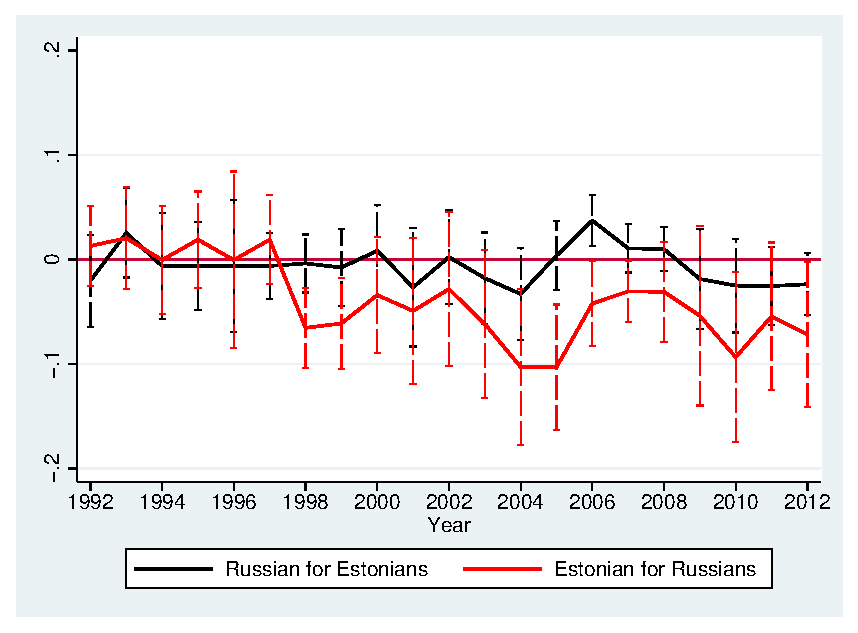
\includegraphics[width=0.45\linewidth]{Figure2a.eps}
%DIFDELCMD < 		\label{fig:long-run_wage_estonian_russian_men}
%DIFDELCMD < 	}
%DIFDELCMD < 	\subfigure[Non-native languages for women]{
%DIFDELCMD < 		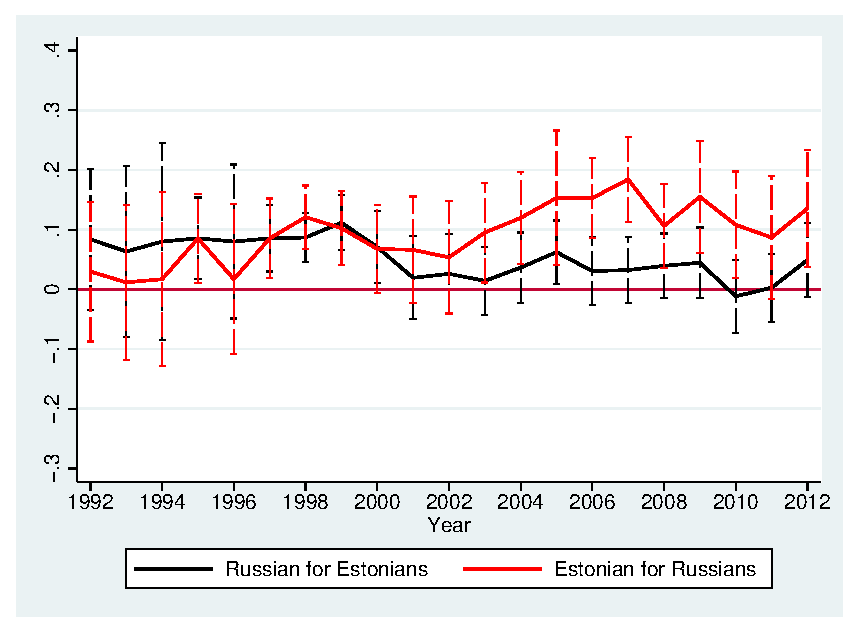
\includegraphics[width=0.45\linewidth]{Figure2b.eps}
%DIFDELCMD < 		\label{fig:long-run_wage_estonian_russian_women}
%DIFDELCMD < 	}
%DIFDELCMD < 	\subfigure[English for Men]{
%DIFDELCMD < 		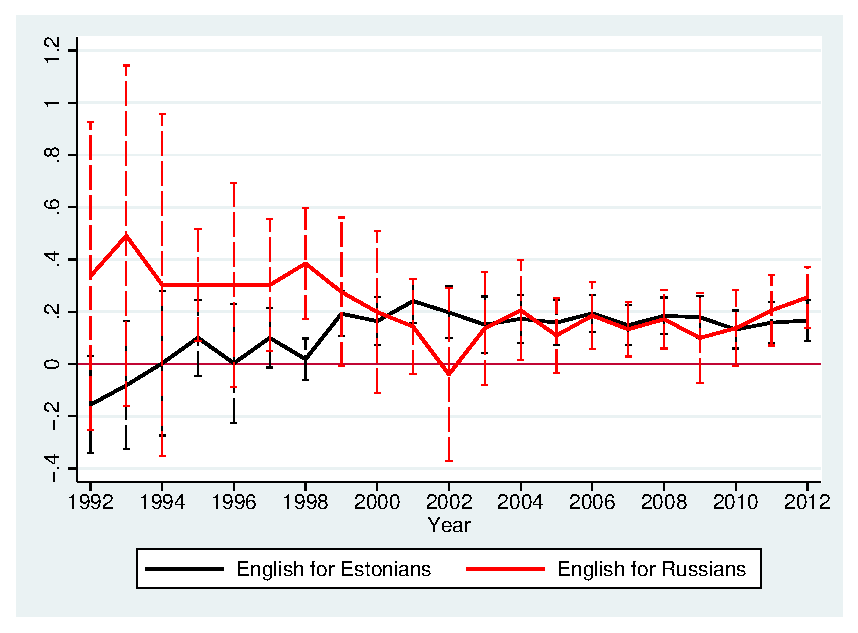
\includegraphics[width=0.45\linewidth]{Figure2c.eps}
%DIFDELCMD < 		\label{fig:long-run_wage_english_men}
%DIFDELCMD < 	}
%DIFDELCMD < 	\subfigure[English for Women]{
%DIFDELCMD < 		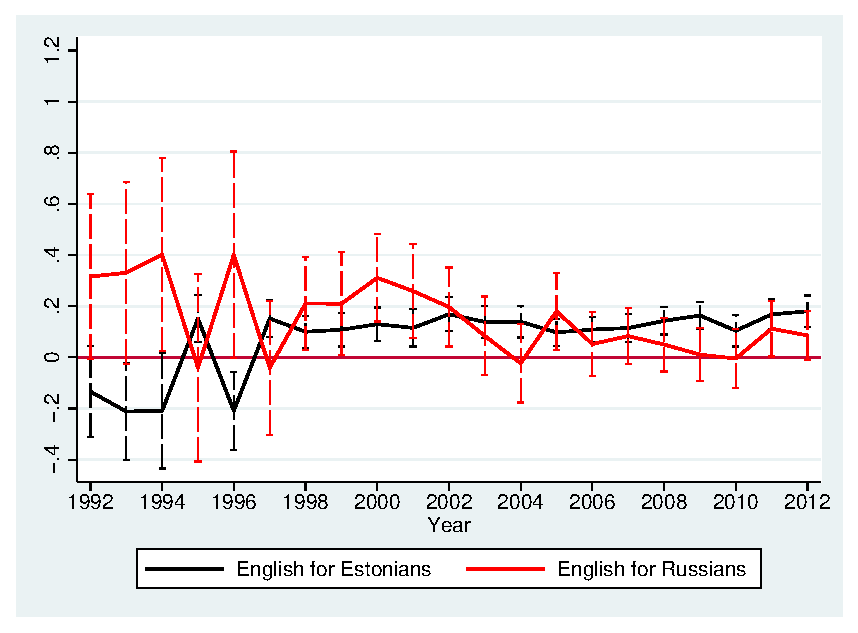
\includegraphics[width=0.45\linewidth]{Figure2d.eps}
%DIFDELCMD < 		\label{fig:long-run_wage_english_women}
%DIFDELCMD < 	}
%DIFDELCMD < 	%%%
\DIFdelendFL \DIFaddbeginFL \subfigure[Non-native languages for men]{
		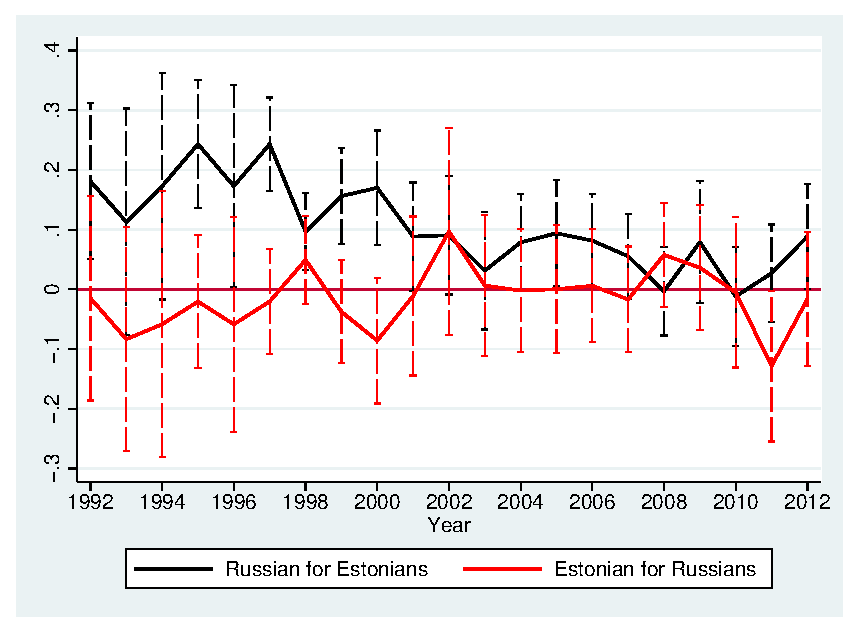
\includegraphics[width=0.45\linewidth]{Figure3a.eps}
		\label{fig:long-run_wage_estonian_russian_men}
	}
	\subfigure[Non-native languages for women]{
		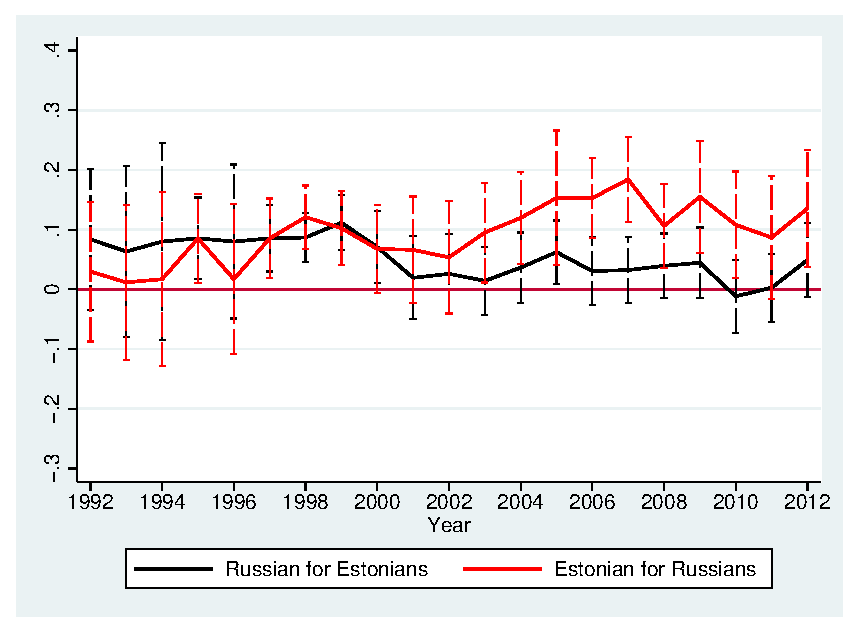
\includegraphics[width=0.45\linewidth]{Figure3b.eps}
		\label{fig:long-run_wage_estonian_russian_women}
	}
	\subfigure[English for Men]{
		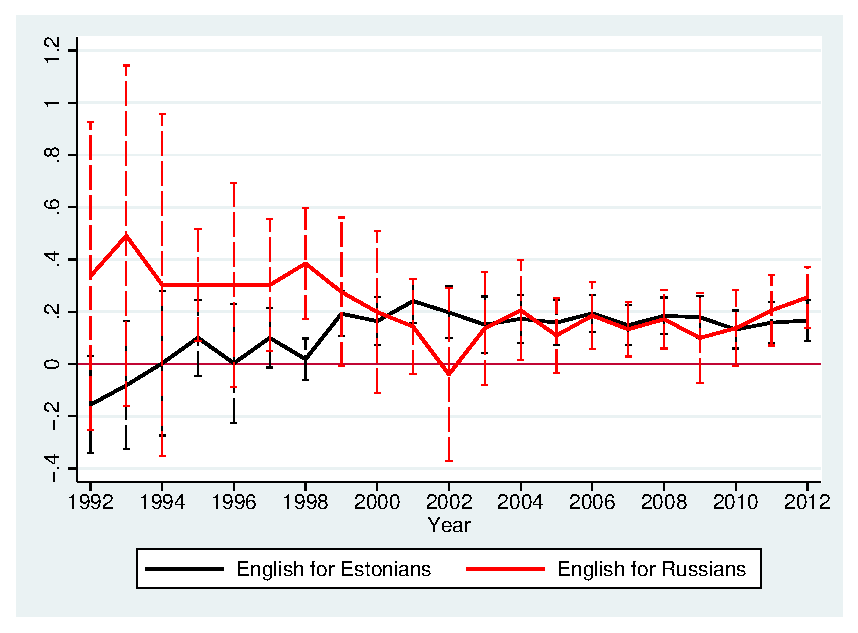
\includegraphics[width=0.45\linewidth]{Figure3c.eps}
		\label{fig:long-run_wage_english_men}
	}
	\subfigure[English for Women]{
		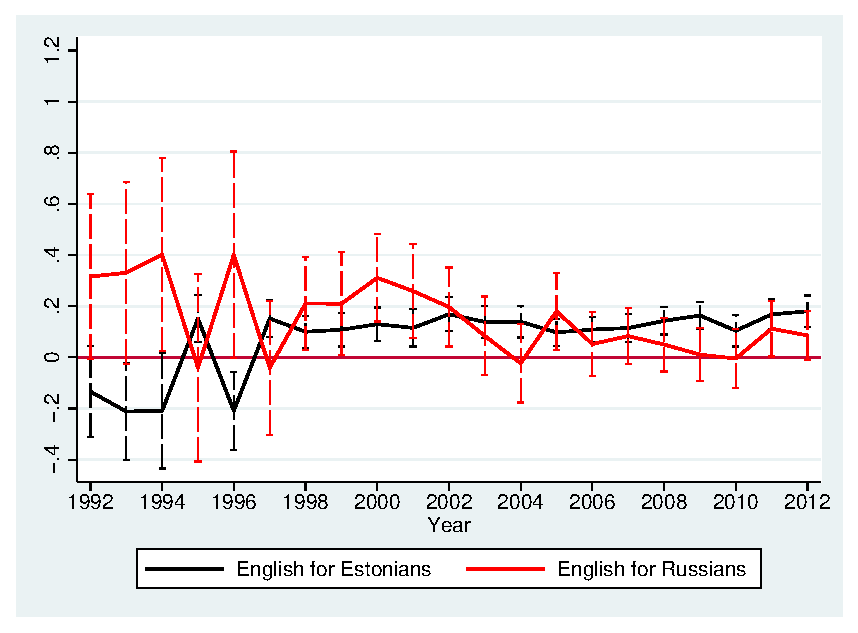
\includegraphics[width=0.45\linewidth]{Figure3d.eps}
		\label{fig:long-run_wage_english_women}
	}
	\DIFaddendFL \caption{The effect of language fluency on wage, 1992--2012\DIFaddbeginFL \DIFaddFL{. }\\ \DIFaddFL{Control variables are \modelTwo. \agerestrictions}\DIFaddendFL }
	\label{fig:long-run_wage}
\end{figure}

The \DIFdelbegin \DIFdel{estimates for wage are rather stable as well}\DIFdelend \DIFaddbegin \DIFadd{wage effects show a similar smooth long-term trend}\DIFaddend . For Estonians, we
see a \DIFdelbegin \DIFdel{slight downward trend of the effect of fluency in Russian whereas
that of }\DIFdelend \DIFaddbegin \DIFadd{slowly fading effect of Russian fluency whereas
}\DIFaddend English becomes important in the late 1990s. For \DIFdelbegin \DIFdel{Russians, the
importance of English seems to be sliding across the years, probably
due to the increasing supply of these skills. For }\DIFdelend \DIFaddbegin \DIFadd{Russian }\DIFaddend men, fluency in Estonian
has never been significantly associated with \DIFdelbegin \DIFdel{wage}\DIFdelend \DIFaddbegin \DIFadd{a wage premium}\DIFaddend .
The results are remarkably stable over the whole period, \DIFdelbegin \DIFdel{stressing
the continuity of the }\DIFdelend \DIFaddbegin \DIFadd{indicating
that the }\DIFaddend peculiar labour market institutions \DIFdelbegin \DIFdel{,
potentially workplace segregation, through the
whole post-communist period. For women, however, }\DIFdelend \DIFaddbegin \DIFadd{have been persistent for
two decades. However, for women }\DIFaddend we can see \DIFdelbegin \DIFdel{a slight increasing trend}\DIFdelend \DIFaddbegin \DIFadd{that Estonian language fluency turned
important in the late 1990s}\DIFaddend , suggesting that there is either less
workplace segregation or \DIFdelbegin \DIFdel{other need for }\DIFdelend \DIFaddbegin \DIFadd{another kind of necessity to know }\DIFaddend the official
language \DIFdelbegin \DIFdel{for
}\DIFdelend \DIFaddbegin \DIFadd{at
}\DIFaddend the jobs commonly taken by women. \DIFaddbegin \DIFadd{The
importance of English seems to be falling over time for Russians, possibly
due to the increasing supply of these skills. 
}\DIFaddend 


\subsection{Does the Effect Differ by Age?}
\label{sec:age_groups}
\DIFdelbegin %DIFDELCMD < 

%DIFDELCMD < %%%
\DIFdel{We also estimate the effects separately by age groups and time in
order to detect potential trends across the age groups
and across ethnic groups
}\DIFdelend \DIFaddbegin \DIFadd{As age is a central determinant of how major economic and political
reforms influence individual careers, 
we also analyse the time trends by age groups
}\DIFaddend (Table~\DIFdelbegin \DIFdel{\ref{tab:age_group_trend_russian} and Table~\ref{tab:age_group_trend_estonian}}\DIFdelend \DIFaddbegin \DIFadd{\ref{tab:age_group_trend}}\DIFaddend ).
We \DIFdelbegin \DIFdel{look separately at }\DIFdelend \DIFaddbegin \DIFadd{group the observation period into }\DIFaddend 4 sub-periods: \DIFdelbegin \DIFdel{Early transition
period
}\DIFdelend \DIFaddbegin \DIFadd{early transition
}\DIFaddend (1989--1995); \DIFdelbegin \DIFdel{First economic growth period }\DIFdelend \DIFaddbegin \DIFadd{first economic growth }\DIFaddend (1996--1999);
\DIFdelbegin \DIFdel{Economic }\DIFdelend \DIFaddbegin \DIFadd{the economic }\DIFaddend boom, EU accession (2000--2007); and the recession
(2008--2012).
\DIFdelbegin %DIFDELCMD < 

%DIFDELCMD < %%%
\DIFdel{We use largely the same setup }\DIFdelend \DIFaddbegin \DIFadd{We use the same econometric framework }\DIFaddend as described in section
\ref{sec:method}\DIFdelbegin \DIFdel{. The }\DIFdelend \DIFaddbegin \DIFadd{, the }\DIFaddend results presented here are \DIFdelbegin \DIFdel{derived using the second model.
}\DIFdelend \DIFaddbegin \DIFadd{based on the specification 2.
}\DIFaddend 

For ethnic Estonians, knowledge of Russian
(Table~\DIFdelbegin \DIFdel{\ref{tab:age_group_trend_estonian}}\DIFdelend \DIFaddbegin \DIFadd{\ref{tab:age_group_trend}, upper panel}\DIFaddend ) has become less
important after its peak in the late 1990s. Notably, the
association between wage and language skills are small in the
\DIFdelbegin \DIFdel{youngest }\DIFdelend \DIFaddbegin \DIFadd{young groups, the }\DIFaddend age groups where \DIFdelbegin \DIFdel{the Russian skills are rapidly declining while it still is strongly related to salary for
older workers. The importance of English language skills fluctuates
and slowly decline through the period, but the men from group }\DIFdelend \DIFaddbegin \DIFadd{knowledge of that language
declining rapidly.
For older age groups, the estimates are larger but not statistically
significant since the recession period. English was not important
during the early years of transition but has been very closely
associated with better pay since 1996. Its importance seems to
fall for the young and middle male groups while the oldest men
}\DIFaddend (45-55) and \DIFdelbegin \DIFdel{young }\DIFdelend \DIFaddbegin \DIFadd{the youngest }\DIFaddend women (25-35) \DIFdelbegin \DIFdel{have }\DIFdelend \DIFaddbegin \DIFadd{show }\DIFaddend a growing trend.
\DIFdelbegin \DIFdel{They gain more from being fluent in }\DIFdelend \DIFaddbegin \DIFadd{This result potentially reflects both the changing supply and demand for 
}\DIFaddend English.

\DIFdelbegin \DIFdel{The positive impact of Estonian language skills for }\DIFdelend \DIFaddbegin \DIFadd{Now we turn to }\DIFaddend ethnic Russians (\DIFdelbegin \DIFdel{Table~\ref{tab:age_group_trend_russian}) on earnings seems to
increase over the sample period for women in the young group (25--35)and the prime age group (36--45). While }\DIFdelend \DIFaddbegin \DIFadd{lower panel in the table). The association between Estonian skills and income shows }\DIFaddend no
statistically significant \DIFdelbegin \DIFdel{correlation is visible for Russian men, good
Estonian is associated with about 10\% higher salary }\DIFdelend \DIFaddbegin \DIFadd{results at all. This is the most unexpected
outcome in our analysis, and we'll return to this
below in Section~\ref{sec:segregation-analysis}.
The effect of Estonian language skills was initially small }\DIFaddend for Russian
women \DIFdelbegin \DIFdel{for the boom in the 2000s. For the
recession period, the figure is even close to 12\% . These age
groups are the workers who were in their twenties or younger during
the major political and economic transition in early 1990s. It
}\DIFdelend \DIFaddbegin \DIFadd{as well, but
since the year 2000, we observe a sizeable gain of approximately
10\% for all subgroups.
The positive outcomes for women for the second decade in our analysis
}\DIFaddend suggests that the previously segregated ``Estonian'' and ``Russian''
\DIFdelbegin \DIFdel{economy }\DIFdelend \DIFaddbegin \DIFadd{economies }\DIFaddend are slowly becoming a more integrated one where ethnic
Russians\DIFdelbegin \DIFdel{with a }\DIFdelend \DIFaddbegin \DIFadd{, at least women, with }\DIFaddend good Estonian command \DIFdelbegin \DIFdel{can get well-paid jobs }\DIFdelend \DIFaddbegin \DIFadd{get better-paid
jobs than those who cannot speak the language}\DIFaddend .
In comparison, the estimates for \DIFdelbegin \DIFdel{English language fluency shows downward trend }\DIFdelend \DIFaddbegin \DIFadd{the English language skills trend downward over
time }\DIFaddend for all age groups for \DIFaddbegin \DIFadd{both }\DIFaddend men and for women. \DIFdelbegin \DIFdel{This is due to the language skills becoming more common among the population}\DIFdelend \DIFaddbegin \DIFadd{A likely
cause is the increasing abundance of these skills over time}\DIFaddend .

\DIFdelbegin %DIFDELCMD < \begin{table}[htbp]
%DIFDELCMD < 	\centering
%DIFDELCMD < 	\caption{The trend over time across the age groups (ethnic Estonians)}
%DIFDELCMD < 	\begin{tabular}{lccc|cc c}
%DIFDELCMD < 		\hline\hline
%DIFDELCMD < 		\multicolumn{7}{l}{Estonian speakers. Dependent variable: log wage}          \\ \hline
%DIFDELCMD < 		Russian:   &    \multicolumn{3}{c|}{Men}    &   \multicolumn{3}{c}{Women}    \\
%DIFDELCMD < 		years/age: & 25-35    & 36-45    & 46-55    & 25-35    & 36-45    & 46-55    \\ \midrule
%DIFDELCMD < 		89-95      & 0.064    & 0.247*** & 0.187*** & 0.117*   & 0.033    & 0.058    \\
%DIFDELCMD < 		           & (0.069)  & (0.068)  & (0.064)  & (0.053)  & (0.057)  & (0.056)  \\
%DIFDELCMD < 		96-99      & 0.116**  & 0.161**  & 0.190*** & 0.059*   & 0.114*** & 0.131*** \\
%DIFDELCMD < 		           & (0.042)  & (0.049)  & (0.054)  & (0.030)  & (0.030)  & (0.033)  \\
%DIFDELCMD < 		00-07      & 0.054*   & 0.157*** & 0.093*   & 0.041    & 0.022    & 0.042    \\
%DIFDELCMD < 		           & (0.026)  & (0.037)  & (0.037)  & (0.024)  & (0.021)  & (0.026)  \\
%DIFDELCMD < 		08-12      & 0.041    & 0.032    & 0.088    & 0.032    & 0.012    & 0.061    \\
%DIFDELCMD < 		           & (0.032)  & (0.049)  & (0.069)  & (0.030)  & (0.026)  & (0.033)  \\ \hline
%DIFDELCMD < 		English:   &          &          &          &          &          &          \\
%DIFDELCMD < 		89-95      & 0.097    & -0.008   & 0.066    & 0.070    & 0.042    & 0.101    \\
%DIFDELCMD < 		           & (0.064)  & (0.065)  & (0.083)  & (0.049)  & (0.048)  & (0.078)  \\
%DIFDELCMD < 		96-99      & 0.190*** & 0.276*** & 0.137*   & 0.113*** & 0.101*** & 0.101**  \\
%DIFDELCMD < 		           & (0.036)  & (0.049)  & (0.054)  & (0.031)  & (0.028)  & (0.038)  \\
%DIFDELCMD < 		00-07      & 0.166*** & 0.158*** & 0.225*** & 0.159*** & 0.073*** & 0.164*** \\
%DIFDELCMD < 		           & (0.027)  & (0.036)  & (0.041)  & (0.024)  & (0.021)  & (0.025)  \\
%DIFDELCMD < 		08-12      & 0.088*   & 0.179*** & 0.236*** & 0.166*** & 0.123*** & 0.145*** \\
%DIFDELCMD < 		           & (0.039)  & (0.035)  & (0.043)  & (0.037)  & (0.024)  & (0.029)  \\ \bottomrule
%DIFDELCMD < 	\end{tabular}
%DIFDELCMD < 	\caption*{ \legend \\ Standard errors (clustered on individuals) in parenthesis}
%DIFDELCMD < 	\label{tab:age_group_trend_estonian}
%DIFDELCMD < \end{table}
%DIFDELCMD < %%%
\DIFdelend \DIFaddbegin \begin{table}[htbp]
	\centering
	\caption{The trend over time across the age groups (ethnic Estonians)}
	\begin{tabular}{lccc|cc c}
     \toprule
		\multicolumn{7}{l}{Estonian speakers. Dependent variable: log wage}     \\ \hline
		Russian:  &  \multicolumn{3}{c|}{Men}  &  \multicolumn{3}{c}{Women}  \\
		years/age: & 25-35  & 36-45  & 46-55  & 25-35  & 36-45  & 46-55  \\ \midrule
		89-95   & 0.064  & 0.247*** & 0.187*** & 0.117*  & 0.033  & 0.058  \\
		      & (0.069) & (0.068) & (0.064) & (0.053) & (0.057) & (0.056) \\
		96-99   & 0.116** & 0.161** & 0.190*** & 0.059*  & 0.114*** & 0.131*** \\
		      & (0.042) & (0.049) & (0.054) & (0.030) & (0.030) & (0.033) \\
		00-07   & 0.054*  & 0.157*** & 0.093*  & 0.041  & 0.022  & 0.042  \\
		      & (0.026) & (0.037) & (0.037) & (0.024) & (0.021) & (0.026) \\
		08-12   & 0.041  & 0.032  & 0.088  & 0.032  & 0.012  & 0.061  \\
		      & (0.032) & (0.049) & (0.069) & (0.030) & (0.026) & (0.033) \\ \hline
		English:  &     &     &     &     &     &     \\
		89-95   & 0.097  & -0.008  & 0.066  & 0.070  & 0.042  & 0.101  \\
		      & (0.064) & (0.065) & (0.083) & (0.049) & (0.048) & (0.078) \\
		96-99   & 0.190*** & 0.276*** & 0.137*  & 0.113*** & 0.101*** & 0.101** \\
		      & (0.036) & (0.049) & (0.054) & (0.031) & (0.028) & (0.038) \\
		00-07   & 0.166*** & 0.158*** & 0.225*** & 0.159*** & 0.073*** & 0.164*** \\
		      & (0.027) & (0.036) & (0.041) & (0.024) & (0.021) & (0.025) \\
		08-12   & 0.088*  & 0.179*** & 0.236*** & 0.166*** & 0.123*** & 0.145*** \\
		      & (0.039) & (0.035) & (0.043) & (0.037) & (0.024) & (0.029) \\ 
     \midrule
		\multicolumn{7}{l}{Russian speakers. Dependent variable: log wage}\\
		\midrule
		Estonian:&\multicolumn{3}{c|}{Men} &\multicolumn{3}{c}{Women}\\
		years/age: & 25-35  & 36-45  & 46-55  & 25-35  & 36-45  & 46-55  \\
		\midrule
		89-95   & -0.027 & -0.113  & -0.029 & 0.134* & 0.073  & -0.039  \\
		      & (0.094) & (0.077) & (0.079) & (0.056) & (0.052) & (0.059) \\
		96-99   & -0.023 & 0.001  & 0.049  & 0.049  & 0.034  & 0.071  \\
		      & (0.050) & (0.048) & (0.060) & (0.045) & (0.035) & (0.037) \\
		00-07   & -0.038 & -0.034  & 0.042  & 0.099** & 0.089** & 0.122*** \\
		      & (0.038) & (0.049) & (0.043) & (0.033) & (0.031) & (0.028) \\
		08-12   & -0.004 & -0.034  & 0.002  & 0.145** & 0.123** & 0.103** \\
		      & (0.055) & (0.050) & (0.047) & (0.051) & (0.044) & (0.038) \\ \midrule
		English:  &     &     &     &     &     & 
           \\

		89-95   & 0.325* & 0.362*  & 0.473* & 0.191  & 0.096  & -0.096  \\
		      & (0.160) & (0.151) & (0.216) & (0.104) & (0.085) & (0.353) \\
		96-99   & 0.324** & 0.224*  & 0.129  & 0.241** & 0.048  & 0.281*  \\
		      & (0.101) & (0.103) & (0.132) & (0.078) & (0.091) & (0.120) \\
		00-07   & 0.142** & 0.107  & 0.169* & 0.127** & 0.104  & 0.127*  \\
		      & (0.051) & (0.097) & (0.072) & (0.049) & (0.060) & (0.057) \\
		08-12   & 0.140* & 0.212*** & 0.138  & 0.029  & 0.105* & 0.040  \\
		      & (0.056) & (0.057) & (0.072) & (0.049) & (0.050) & (0.055) \\
		\bottomrule
	\end{tabular}

	\caption*{\legend \\ Standard errors (clustered on individuals) in parenthesis. \\ Individual characteristics are \modelTwo. 	}
	\label{tab:age_group_trend}
\end{table}
\DIFaddend 

\DIFdelbegin %DIFDELCMD < \begin{table}[t!]
%DIFDELCMD < 	\centering
%DIFDELCMD < 	\caption{The trend over time across the age groups (ethnic
%DIFDELCMD < 		Russians)}
%DIFDELCMD < 	\begin{tabular}{lccc|cc c}
%DIFDELCMD < 		\hline\hline
%DIFDELCMD < 		\multicolumn{7}{l}{Russian speakers. Dependent variable: log wage}\\
%DIFDELCMD < 		\midrule
%DIFDELCMD < 		Estonian:&\multicolumn{3}{c|}{Men} &\multicolumn{3}{c}{Women}\\
%DIFDELCMD < 		years/age: & 25-35   & 36-45    & 46-55   & 25-35   & 36-45   & 46-55    \\
%DIFDELCMD < 		\midrule
%DIFDELCMD < 		89-95      & -0.027  & -0.113   & -0.029  & 0.134*  & 0.073   & -0.039   \\
%DIFDELCMD < 		           & (0.094) & (0.077)  & (0.079) & (0.056) & (0.052) & (0.059)  \\
%DIFDELCMD < 		96-99      & -0.023  & 0.001    & 0.049   & 0.049   & 0.034   & 0.071    \\
%DIFDELCMD < 		           & (0.050) & (0.048)  & (0.060) & (0.045) & (0.035) & (0.037)  \\
%DIFDELCMD < 		00-07      & -0.038  & -0.034   & 0.042   & 0.099** & 0.089** & 0.122*** \\
%DIFDELCMD < 		           & (0.038) & (0.049)  & (0.043) & (0.033) & (0.031) & (0.028)  \\
%DIFDELCMD < 		08-12      & -0.004  & -0.034   & 0.002   & 0.145** & 0.123** & 0.103**  \\
%DIFDELCMD < 		           & (0.055) & (0.050)  & (0.047) & (0.051) & (0.044) & (0.038)  \\ \midrule
%DIFDELCMD < 		English:   &         &          &         &         &         &          \\
%DIFDELCMD < 		89-95      & 0.325*  & 0.362*   & 0.473*  & 0.191   & 0.096   & -0.096   \\
%DIFDELCMD < 		           & (0.160) & (0.151)  & (0.216) & (0.104) & (0.085) & (0.353)  \\
%DIFDELCMD < 		96-99      & 0.324** & 0.224*   & 0.129   & 0.241** & 0.048   & 0.281*   \\
%DIFDELCMD < 		           & (0.101) & (0.103)  & (0.132) & (0.078) & (0.091) & (0.120)  \\
%DIFDELCMD < 		00-07      & 0.142** & 0.107    & 0.169*  & 0.127** & 0.104   & 0.127*   \\
%DIFDELCMD < 		           & (0.051) & (0.097)  & (0.072) & (0.049) & (0.060) & (0.057)  \\
%DIFDELCMD < 		08-12      & 0.140*  & 0.212*** & 0.138   & 0.029   & 0.105*  & 0.040    \\
%DIFDELCMD < 		           & (0.056) & (0.057)  & (0.072) & (0.049) & (0.050) & (0.055)  \\
%DIFDELCMD < 		\bottomrule
%DIFDELCMD < 	\end{tabular}
%DIFDELCMD < 

%DIFDELCMD < 	\caption*{\legend \\ Standard errors (clustered on individuals) in parenthesis}
%DIFDELCMD < 	\label{tab:age_group_trend_russian}
%DIFDELCMD < \end{table}
%DIFDELCMD < 

%DIFDELCMD < %%%
\DIFdel{We estimate the effect of language skills for unemployment as well for the second model.
Howevertoo little results are statistically significant. The importance of Estonian language skills was growing during the latest periods and is associated with approximately 7 percentage points lower unemployment for both Russian men and women. 
The best results are reached for the
youngest age groups and }\DIFdelend \DIFaddbegin \DIFadd{We repeat the exercise for the unemployment models.
However, due to relatively small groups, most of the results are not
statistically significant and we
do not report those here.
}



\section{\DIFadd{Additional Evidence: Education and Workplace}}
\label{sec:segregation-analysis}

\DIFadd{The most surprising result in our analysis so far -- the fact that
Russian men earn virtually no Estonian language premium while women do -- warrants a
deeper look at the data. We split the average wage for the Russian male wage-earners
along three
dimensions: Estonian language skills (}\emph{\DIFadd{EST 0}} \DIFadd{and }\emph{\DIFadd{EST 1}}\DIFadd{),
residence in Tallinn metro area (}\emph{\DIFadd{Tallinn}} \DIFadd{and }\emph{\DIFadd{Other}}\DIFadd{),
and education (}\emph{\DIFadd{< HS}}\DIFadd{, }\emph{\DIFadd{HS}}\DIFadd{, }\emph{\DIFadd{College Degree}}\DIFadd{). The metropolitan area is one of the two major regions
where the Russian-speaking population is concentrated, and its
booming economy may be very different from the other such region, the
North-East (Ida-Virumaa), and the rest of the country.
In order to correct for the strong wage and language skill trends
through the observation period, we do not present the average wage,
but instead the respective OLS residuals where we explain the log wage by year fixed
effects and include no other explanatory variables (Table~\ref{tab:loc-lang-edu}). 
}

\DIFadd{The table shows that the picture is in fact complex. We can see
that there is little to no gain from Estonian skills for the
largest group of workers, those with a high school degree. Even more, outside of
the metropolitan area, the lowest and highest education groups
have in fact negative language premium. However, these two groups
enjoy quite a noticeable premium in the Tallinn region. The
opposite-signed effects in for these two education groups suggests
that a
selective internal migration may play a role.
}

%DIF >  latex table generated in R 3.4.4 by xtable 1.8-2 package
%DIF >  Fri Jul 6 15:59:47 2018
\begin{table}[ht]
 \centering
 \textcolor{Blue}{
 \caption{\color{Blue} Average wage and time-trend corrected residual across
  location and education groups for Russian men}
 \begin{tabular}{llrrrr}
  \toprule
  & & &\multicolumn{2}{c}{Log Wage}\\
  Location & Education & \# Observations & EST 0 & EST 1 & Premium\\
  \midrule
  Tallinn & $<$ HS & 399 & -0.20 & -0.01 & 0.19 \\ 
  Tallinn & HS & 2164 & 0.07 & 0.04 & -0.03 \\ 
  Tallinn & College Degree & 610 & 0.15 & 0.30 & 0.15 \\ 
  Other & $<$ HS & 501 & -0.12 & -0.12 & -0.01 \\ 
  Other & HS & 2658 & -0.10 & -0.07 & 0.03 \\ 
  Other & College Degree & 429 & 0.17 & 0.11 & -0.06 \\ 
  \bottomrule
 \end{tabular}
 \begin{flushleft}
  Notes: \emph{Log Wage} refers to regression residual where log
  wage is explained by year fixed effects. \emph{EST 0} and
  \emph{EST 1} are mean values for those who cannot, and who can,
  speak Estonian; $\text{Premium} = \text{EST 1} - \text{EST 0}$.
  Education level \emph{< HS} refers to less than high school
  degree, \emph{HS} is the high school degree as the highest
  completed education.
 \end{flushleft}
}
 \label{tab:loc-lang-edu}
\end{table}

\DIFadd{We can conclude from the Table~\ref{tab:loc-lang-edu} that our
most surprising finding, no positive effect of Estonian language
skills }\DIFaddend for \DIFdelbegin \DIFdel{middle age groups .
English skills are related to less unemployment both for }\DIFdelend Russian men\DIFdelbegin \DIFdel{and women. The effect is smaller for Estonian men while for Estonian women all results are insignificant}\DIFdelend \DIFaddbegin \DIFadd{, is primarily driven by the largest group, workers with
a high school degree. It also suggests that highly educated workers in
the metropolitan area enjoy, in fact, a substantial language premium.
However, this group is not very large}\DIFaddend .

\DIFdelbegin \section{\DIFdel{Additional Evidence: Estonian Language at Workplace}}
%DIFAUXCMD
\addtocounter{section}{-1}%DIFAUXCMD
%DIFDELCMD < \label{sec:segregation_analysis}
%DIFDELCMD < 

%DIFDELCMD < %%%
\DIFdel{Previous }\DIFdelend \DIFaddbegin \DIFadd{The previous }\DIFaddend results can be explained by \DIFaddbegin \DIFadd{a combination of }\DIFaddend two hypotheses: first,
Russian--speaking men\DIFaddbegin \DIFadd{, at least those with high school degree as their
highest completed education level, }\DIFaddend are working
primarily in Russian language environment \DIFaddbegin \DIFadd{(ethnic segregation) }\DIFaddend while this is not true for
women; and second, Russian-speaking men are working in jobs with
little communication requirements (gender segregation).
\DIFdelbegin %DIFDELCMD < 

%DIFDELCMD < %%%
\DIFdel{To shed some additional light }\DIFdelend \DIFaddbegin \DIFadd{To get some additional evidence }\DIFaddend on these hypotheses, we use data
from \DIFaddbegin \DIFadd{the }\DIFaddend 2008 Integration Monitor Survey. We focus on
two questions: ``which is the language of communication at your
workplace?'' and ``which languages do you need at work''. The first
question addresses the ethnic segregation while the second focuses on
the need of \DIFdelbegin \DIFdel{communication.  As very few individuals work in English
environment, we only look for Estonian as the communication language }\DIFdelend \DIFaddbegin \DIFadd{the language for communication}\DIFaddend . 

\DIFdelbegin %DIFDELCMD < \begin{table}[t]
%DIFDELCMD < 	\centering
%DIFDELCMD < 	\caption{Language environment and language need at workplace}
%DIFDELCMD < 	\label{tab:environment_descriptive}
%DIFDELCMD < 	\begin{tabular}{lrr}
%DIFDELCMD < 		\toprule
%DIFDELCMD < 		                                     & men  & women \\
%DIFDELCMD < 		\midrule
%DIFDELCMD < 		main communication language Estonian & 15.0 & 22.2  \\
%DIFDELCMD < 		Need Estonian at work                & 53.0 & 61.9  \\
%DIFDELCMD < 		Need English  at work                & 26.5 & 11.9  \\
%DIFDELCMD < 		\midrule
%DIFDELCMD < 		observations                         & 132  & 134   \\
%DIFDELCMD < 		\bottomrule
%DIFDELCMD < 	\end{tabular}
%DIFDELCMD < 	\begin{flushleft}
%DIFDELCMD < 		Note: percentage of respondents who respond affirmatively
%DIFDELCMD < 	\end{flushleft}
%DIFDELCMD < \end{table}
%DIFDELCMD < %%%
\DIFdelend \DIFaddbegin \begin{table}[t]         
	\centering
	\caption{Language environment and language need at workplace}
	\label{tab:environment_descriptive}
	\begin{tabular}{lrr}
		\toprule
		                   & men & women \\
		\midrule
		main communication language Estonian & 15.0 & 22.2 \\
		Need Estonian at work        & 53.0 & 61.9 \\
		Need English at work        & 26.5 & 11.9 \\
		\midrule
		\# Observations             & 132 & 134  \\
		\bottomrule
	\end{tabular}
	\begin{flushleft}
		Note: percentage of respondents who respond affirmatively
	\end{flushleft}
\end{table}
\DIFaddend 

Table~\ref{tab:environment_descriptive} shows the proportion of
Russian respondents who use Estonian as the main communication language at work, and
who need Estonian and English at work. As we see, women are more likely to
use Estonian \DIFdelbegin \DIFdel{than men }\DIFdelend while the opposite is true for English.
Table~\ref{tab:environment_model} presents the \DIFdelbegin \DIFdel{regression results when
controlling for other
}\DIFdelend \DIFaddbegin \DIFadd{corresponding regression results
where we estimate the likelihood of having the need for and using the
language at work
while
controlling for gender and other individual
}\DIFaddend characteristics, including education and geographic location.

\DIFdelbegin %DIFDELCMD < \begin{table}[t]
%DIFDELCMD < 	\centering
%DIFDELCMD < 	\caption{Language environment and language need at workplace:
%DIFDELCMD < 		regression results}
%DIFDELCMD < 	\label{tab:environment_model}
%DIFDELCMD < 	\begin{tabular}{l r@{}l r@{}l r@{}l}
%DIFDELCMD < 		\toprule
%DIFDELCMD < 		Dependent variable: & \multicolumn{2}{c}{Need Estonian} & \multicolumn{2}{c}{Use Estonian} & \multicolumn{2}{c}{Need English} \\ \midrule
%DIFDELCMD < 		woman             & 0.262       & **  & 0.162       & *   & -0.045      &   \\
%DIFDELCMD < 		                  & \std{0.117} &     & \std{0.095} &     & \std{0.192} &   \\
%DIFDELCMD < 		college education & 0.201       & **  & 0.132       & **  & 0.133       & * \\
%DIFDELCMD < 		                  & \std{0.083} &     & \std{0.067} &     & \std{0.079} &   \\
%DIFDELCMD < 		region Tallinn    & -0.276      & *** & -0.463      & *** & 0.036       &   \\
%DIFDELCMD < 		                  & \std{0.083} &     & \std{0.067} &     & \std{0.080} &   \\
%DIFDELCMD < 		region North-East & -0.527      & *** & -0.473      & *** & 0.022       &   \\
%DIFDELCMD < 		                  & \std{0.091} &     & \std{0.074} &     & \std{0.088} &   \\ \midrule
%DIFDELCMD < 		N obs             & 228         &     & 228         &     & 228         &   \\
%DIFDELCMD < 		$R^{2}$           & 0.2598      &     & 0.2831      &     & 0.108       &   \\ \bottomrule
%DIFDELCMD < 	\end{tabular}
%DIFDELCMD < 	\begin{flushleft}
%DIFDELCMD < 		Note: control variables include: marital status, education,
%DIFDELCMD < 		occupation and age.
%DIFDELCMD < 	\end{flushleft}
%DIFDELCMD < \end{table}
%DIFDELCMD < %%%
\DIFdelend \DIFaddbegin \begin{table}[t]
	\centering
	\caption{Language environment and language need at workplace:
		regression results}
	\label{tab:environment_model}
	\begin{tabular}{l r@{}l r@{}l r@{}l}
		\toprule
		Dependent variable: & \multicolumn{2}{c}{Need Estonian} & \multicolumn{2}{c}{Use Estonian} & \multicolumn{2}{c}{Need English} \\ \midrule
		woman       & 0.262    & ** & 0.162    & *  & -0.045   &  \\
		         & \std{0.117} &   & \std{0.095} &   & \std{0.192} &  \\
		college education & 0.201    & ** & 0.132    & ** & 0.133    & * \\
		         & \std{0.083} &   & \std{0.067} &   & \std{0.079} &  \\
		region Tallinn  & -0.276   & *** & -0.463   & *** & 0.036    &  \\
		         & \std{0.083} &   & \std{0.067} &   & \std{0.080} &  \\
		region North-East & -0.527   & *** & -0.473   & *** & 0.022    &  \\
		         & \std{0.091} &   & \std{0.074} &   & \std{0.088} &  \\ \midrule
		\# Observations       & 228     &   & 228     &   & 228     &  \\
		$R^{2}$      & 0.2598   &   & 0.2831   &   & 0.108    &  \\ \bottomrule
	\end{tabular}
	\begin{flushleft}
		Note: control variables include: marital status, education,
		occupation and age.
	\end{flushleft}
\end{table}
\DIFaddend 

The table indicates that Russian women need Estonian 26 percentage
points more at work than Russian men. The table also suggests that
Russian women are 16 percentage points more likely to be working in
Estonian-speaking environment when controlling for other factors.
Both \DIFdelbegin \DIFdel{estimates }\DIFdelend \DIFaddbegin \DIFadd{figures }\DIFaddend are statistically significant (at 5\% and 10 \% level
respectively), \DIFdelbegin \DIFdel{but not precisely estimated}\DIFdelend \DIFaddbegin \DIFadd{although the standard errors are large}\DIFaddend . We can also see that
college education is associated by much more Estonian need and usage,
but in regions where Russian speakers are concentrated, the capital
Tallinn and the North-East, Estonian is less needed. In contrast, no
gender difference is visible for English needs.

In summary, this dataset supports \DIFdelbegin \DIFdel{the previous hypothesis}\DIFdelend \DIFaddbegin \DIFadd{both of the hypotheses outlined above}\DIFaddend : Russian women are
working in \DIFaddbegin \DIFadd{a }\DIFaddend less segregated environment where Estonian is the main
communication language \DIFdelbegin \DIFdel{, }\DIFdelend and they need Estonian \DIFaddbegin \DIFadd{at work }\DIFaddend for other reasons as
well. Gender differences in English usage are not statistically
significant.


\DIFdelbegin \DIFdel{Additionally we briefly analysed online job market }%DIFDELCMD < \href{http://www.cv.ee/english/}{cv.ee}%%%
\DIFdel{.  We measured all jobs
that required English, Finnish and Russian, and calculated the average education requirement
at these jobs (coded as college/less than college education).  According to the observations,
the jobs that required English, in average, 51\% of college education while those where Finnish is requested, 19\% and Russian is 26\% respectively.
}%DIFDELCMD < 

%DIFDELCMD < %%%
\DIFdelend \section{Discussion and Concluding Remarks}
\label{sec:discussion}

We document that \DIFdelbegin \DIFdel{different languages are associated in a
different way }\DIFdelend \DIFaddbegin \DIFadd{all analysed language skills are associated }\DIFaddend with
unemployment and wage\DIFaddbegin \DIFadd{, however in a different way}\DIFaddend . Our most
intriguing observation is that \DIFdelbegin \DIFdel{Russian men }\DIFdelend \DIFaddbegin \DIFadd{the largest group of
Russian men, high school graduates, }\DIFaddend earn virtually no income premium \DIFdelbegin \DIFdel{from being }\DIFdelend \DIFaddbegin \DIFadd{if }\DIFaddend fluent in Estonian,
the majority and \DIFaddbegin \DIFadd{the }\DIFaddend official language of the country, while \DIFdelbegin \DIFdel{the fluency }\DIFdelend \DIFaddbegin \DIFadd{ability
to speak the language }\DIFaddend is related to a substantially
lower unemployment rate.
Our analysis supports \citet{YaoandOurs2015}\DIFaddbegin \DIFadd{, }\DIFaddend and \citet{Lindemann2013} \DIFdelbegin \DIFdel{finding }\DIFdelend \DIFaddbegin \DIFadd{findings }\DIFaddend that 
the labour market is segmented between ethnic and gender lines.
However, we find that ethnic segregation is less prevalent \DIFdelbegin \DIFdel{at the lower end
of the }\DIFdelend \DIFaddbegin \DIFadd{in the }\DIFaddend male
labour market.
\DIFdelbegin \DIFdel{The lower--end labour market, associated with frequent unemployment, is
better integrated and
those who are fluent in the language may expect both less unemployment
and higher wage.  However, menat better paid and more stable jobs
gain little from Estonian
.  We
suppose this is because the middle and upper-end labour market is more
segregated and even
those who speak the official language cannot improve their income
much.  This is possibly a type of glass-ceiling effect.  This hypothesis is
supported by }\DIFdelend \DIFaddbegin \DIFadd{This suggests for the majority of Russian speaking men, Estonian
language gives a distinct advantage by facilitating hiring by
Estonian-dominated employers. We also confirm
}\DIFaddend \citet{leppik+vihalemm2015JofBaltStud} \DIFdelbegin \DIFdel{who show that
Estonian language skills are not associated with improved career mobilityover time. It is also corroborated with the quantile regression evidence that
Estonian language is related to a positive wage premium only at the
lowest end of income scale }%DIFDELCMD < \citep{Toomet2011}%%%
\DIFdelend \DIFaddbegin \DIFadd{conclusion that
these
jobs are associated with little career mobility}\DIFaddend . There is also \DIFaddbegin \DIFadd{some
}\DIFaddend anecdotal evidence suggesting that offices are
typically manned by ethnic Estonians while \DIFdelbegin \DIFdel{production }\DIFdelend \DIFaddbegin \DIFadd{manufacturing }\DIFaddend units have a
large share of Russian workers.
One can speculate that this outcome is related to a substantial population share
with negative attitudes toward Russians \citep{korts2009JofBaltStud}.
\DIFaddbegin \DIFadd{On a more positive tone, we find
that this may not be the case for highly educated workers.
}\DIFaddend 

The ethnic segregation seems to be less of an issue for women.
Unfortunately, neither \citet{Toomet2011} nor
\citet{leppik+vihalemm2015JofBaltStud} analyse men and women
separately. We \DIFdelbegin \DIFdel{suppose that }\DIFdelend \DIFaddbegin \DIFadd{find some evidence that female labor market is less
segregated along ethnic lines, and }\DIFaddend women are more frequently employed in jobs in which they need Estonian
language more, such as working in a direct contact with customers.
We also find evidence that over time Estonian is becoming more
important in the female labour market. Unfortunately, the current data
does not let us \DIFdelbegin \DIFdel{to }\DIFdelend assess whether is due to decreasing segregation, or
economy--wide rise of \DIFaddbegin \DIFadd{the importance of }\DIFaddend Estonian language. No such trend is visible for
men \DIFaddbegin \DIFadd{suggesting that 20 years ---almost a generation--- after
establishing a nation state and market economy, the
labour market integration is still not complete}\DIFaddend .

The \DIFaddbegin \DIFadd{fact that the Russian language is not associated with any better
employment prospects
is in stark contrast to the results by }\citet{Alan2015}\DIFadd{. This is
potentially related to the sharp re-orientation to Western markets and
nation-state related political reforms Estonia experienced in the
early 1990s. Rapid withdrawal from the former USSR economy has
resulted in
a laudable economic growth, but may have led to
increased ethnic disparities, compared to the economies that moved in
a slower pace, such as Ukraine }\citep{Constant2011} \DIFadd{and the former Caucasus republics
}\citep{Alan2015}\DIFadd{. 
}

\DIFadd{Our }\DIFaddend other results are more in line with other studies.
English language \DIFaddbegin \DIFadd{fluency }\DIFaddend is related to a substantial income premium but
\DIFdelbegin \DIFdel{virtually to }\DIFdelend \DIFaddbegin \DIFadd{to virtually }\DIFaddend no effect on unemployment. This is similar to findings by
\citet{ginsburgh+prieto-rodriguez2011ILRR} and \DIFdelbegin %DIFDELCMD < \citet{beblavy+2016CEPS} %%%
\DIFdelend \DIFaddbegin \DIFadd{\mbox{%DIFAUXCMD
\cite{fabo+2017E}
}\hspace{0pt}%DIFAUXCMD
}\DIFaddend who show that English is more important at \DIFdelbegin \DIFdel{better paid
}\DIFdelend \DIFaddbegin \DIFadd{better-paid
}\DIFaddend jobs. In contrast, our outcomes suggest that English has little use
at \DIFdelbegin \DIFdel{low-paid, unstable jobs}%DIFDELCMD < \citep{Toomet2011}%%%
\DIFdel{.
}%DIFDELCMD < 

%DIFDELCMD < %%%
\DIFdelend \DIFaddbegin \DIFadd{unstable jobs, at these jobs where workers frequently move between
employment and unemployment.
}\DIFaddend Note also that \DIFdelbegin \DIFdel{for
}\DIFdelend \DIFaddbegin \DIFadd{in case of
}\DIFaddend English, we are able to explain a substantial part of the raw effect
by individual characteristics, suggesting that the true causal effect
may be smaller than our estimates.

The study has \DIFdelbegin \DIFdel{a number of }\DIFdelend \DIFaddbegin \DIFadd{two main }\DIFaddend limitations. Although we believe that our
estimates are good indicators of a causal relationship, we cannot \DIFdelbegin \DIFdel{make
such claim unless a suitable instruments for language skills can be
found}\DIFdelend \DIFaddbegin \DIFadd{be
sure this is the case as our data do not contain strong enough instruments}\DIFaddend .
In particular, as individual characteristics are able to explain a
large part of English returns, we suppose part of the remaining effect
may also \DIFaddbegin \DIFadd{be }\DIFaddend related to an ability bias. Another weak point in the current
data \DIFdelbegin \DIFdel{, although it is
standard in the literature, is using the }\DIFdelend \DIFaddbegin \DIFadd{are the }\DIFaddend self-reported language
skills. As language test data becomes available, we may be able to
decrease the measurement error in the future.


\bibliographystyle{apacite}
\begin{thebibliography}{}

\bibitem [\protect \citeauthoryear {%
Armstrong%
}{%
Armstrong%
}{%
{\protect \APACyear {2015}}%
}]{%
Armstrong2015}
\APACinsertmetastar {%
Armstrong2015}%
\begin{APACrefauthors}%
Armstrong, A.%
\end{APACrefauthors}%
\unskip\
\newblock
\APACrefYearMonthDay{2015}{}{}.
\newblock
{\BBOQ}\APACrefatitle {Equilibria and efficiency in bilingual labour markets}
  {Equilibria and efficiency in bilingual labour markets}.{\BBCQ}
\newblock
\APACjournalVolNumPages{Journal of Economic Behavior \&
  Organization}{112}{}{204 - 220}.
\newblock
\begin{APACrefURL}
  \url{http://www.sciencedirect.com/science/article/pii/S0167268115000359}
  \end{APACrefURL}
\newblock
\begin{APACrefDOI} \doi{http://dx.doi.org/10.1016/j.jebo.2015.01.011}
  \end{APACrefDOI}
\PrintBackRefs{\CurrentBib}

\bibitem [\protect \citeauthoryear {%
Azam%
, Chin%
\BCBL {}\ \BBA {} Prakash%
}{%
Azam%
\ \protect \BOthers {.}}{%
{\protect \APACyear {2013}}%
}]{%
azam+2013EDandCC}
\APACinsertmetastar {%
azam+2013EDandCC}%
\begin{APACrefauthors}%
Azam, M.%
, Chin, A.%
\BCBL {}\ \BBA {} Prakash, N.%
\end{APACrefauthors}%
\unskip\
\newblock
\APACrefYearMonthDay{2013}{}{}.
\newblock
{\BBOQ}\APACrefatitle {The Returns to {E}nglish-Language Skills in {I}ndia}
  {The returns to {E}nglish-language skills in {I}ndia}.{\BBCQ}
\newblock
\APACjournalVolNumPages{Economic Development and Cultural
  Change}{61}{2}{335-367}.
\newblock
\begin{APACrefURL} \url{http://www.jstor.org/stable/10.1086/668277}
  \end{APACrefURL}
\PrintBackRefs{\CurrentBib}

\DIFdelbegin %DIFDELCMD < \bibitem [\protect \citeauthoryear {%
%DIFDELCMD < Beblavý%
%DIFDELCMD < , Fabo%
%DIFDELCMD < \BCBL {}\ \BBA {} Lenaerts%
%DIFDELCMD < }{%
%DIFDELCMD < Beblavý%
%DIFDELCMD < \ \protect \BOthers {.}}{%
%DIFDELCMD < {\protect \APACyear {2016}}%
%DIFDELCMD < }]{%
%DIFDELCMD < beblavy+2016CEPS}
%DIFDELCMD < \APACinsertmetastar {%
%DIFDELCMD < beblavy+2016CEPS}%%%
%DIF < 
%DIFDELCMD < \begin{APACrefauthors}%%%
%DIF < 
\DIFdel{Beblavý, M.%DIF < 
, Fabo, B.%DIF < 
}%DIFDELCMD < \BCBL {}%%%
\DIFdel{\ }%DIFDELCMD < \BBA {} %%%
\DIFdel{Lenaerts, K.%DIF < 
}%DIFDELCMD < \end{APACrefauthors}%%%
%DIF < 
%DIFDELCMD < \unskip%%%
\DIFdel{\
}%DIFDELCMD < \newblock
%DIFDELCMD < \APACrefYearMonthDay{2016}{1}{}%%%
\DIFdel{.
}%DIFDELCMD < \newblock
%DIFDELCMD < \APACrefbtitle {The Importance of Foreign Language Skills in the Labour Markets
%DIFDELCMD <   of Central and Eastern Europe: An assessment based on data from online job
%DIFDELCMD <   portals.} {The importance of foreign language skills in the labour markets of
%DIFDELCMD <   central and eastern europe: An assessment based on data from online job
%DIFDELCMD <   portals.}%%%
\DIFdel{\ }%DIFDELCMD < \APACbVolEdTR {}{Special Report\ \BNUM~129}%%%
\DIFdel{.
}%DIFDELCMD < \newblock
%DIFDELCMD < \APACaddressInstitution{Brussels}{CEPS}%%%
\DIFdel{.
}%DIFDELCMD < \PrintBackRefs{\CurrentBib}
%DIFDELCMD < 

%DIFDELCMD < %%%
\DIFdelend \bibitem [\protect \citeauthoryear {%
Bellante%
\ \BBA {} Kogut%
}{%
Bellante%
\ \BBA {} Kogut%
}{%
{\protect \APACyear {1998}}%
}]{%
Bellante1998}
\APACinsertmetastar {%
Bellante1998}%
\begin{APACrefauthors}%
Bellante, D.%
\BCBT {}\ \BBA {} Kogut, C\BPBI A.%
\end{APACrefauthors}%
\unskip\
\newblock
\APACrefYearMonthDay{1998}{}{}.
\newblock
{\BBOQ}\APACrefatitle {Language ability, US labor market experience and the
  earnings of immigrants} {Language ability, us labor market experience and the
  earnings of immigrants}.{\BBCQ}
\newblock
\APACjournalVolNumPages{International Journal of Manpower}{19}{5}{319-330}.
\newblock
\begin{APACrefURL} \url{http://dx.doi.org/10.1108/01437729810221995}
  \end{APACrefURL}
\newblock
\begin{APACrefDOI} \doi{10.1108/01437729810221995} \end{APACrefDOI}
\PrintBackRefs{\CurrentBib}

\bibitem [\protect \citeauthoryear {%
Bleakley%
\ \BBA {} Chin%
}{%
Bleakley%
\ \BBA {} Chin%
}{%
{\protect \APACyear {2004}}%
}]{%
bleakley+chin2004}
\APACinsertmetastar {%
bleakley+chin2004}%
\begin{APACrefauthors}%
Bleakley, H.%
\BCBT {}\ \BBA {} Chin, A.%
\end{APACrefauthors}%
\unskip\
\newblock
\APACrefYearMonthDay{2004}{}{}.
\newblock
{\BBOQ}\APACrefatitle {Language skills and earnings: Evidence from childhood
  immigrants} {Language skills and earnings: Evidence from childhood
  immigrants}.{\BBCQ}
\newblock
\APACjournalVolNumPages{Review of Economics and Statistics}{86}{2}{481-496}.
\PrintBackRefs{\CurrentBib}

\bibitem [\protect \citeauthoryear {%
Casale%
\ \BBA {} Posel%
}{%
Casale%
\ \BBA {} Posel%
}{%
{\protect \APACyear {2011}}%
}]{%
Casale2011}
\APACinsertmetastar {%
Casale2011}%
\begin{APACrefauthors}%
Casale, D.%
\BCBT {}\ \BBA {} Posel, D.%
\end{APACrefauthors}%
\unskip\
\newblock
\APACrefYearMonthDay{2011}{}{}.
\newblock
{\BBOQ}\APACrefatitle {English language proficiency and earnings in a
  developing country: The case of South Africa} {English language proficiency
  and earnings in a developing country: The case of south africa}.{\BBCQ}
\newblock
\APACjournalVolNumPages{The Journal of Socio-Economics}{40}{4}{385-393}.
\newblock
\begin{APACrefURL}
  \url{http://EconPapers.repec.org/RePEc:eee:soceco:v:40:y:2011:i:4:p:385-393}
  \end{APACrefURL}
\PrintBackRefs{\CurrentBib}

\DIFdelbegin %DIFDELCMD < \bibitem [\protect \citeauthoryear {%
%DIFDELCMD < B.~Chiswick%
%DIFDELCMD < \ \BBA {} Miller%
%DIFDELCMD < }{%
%DIFDELCMD < B.~Chiswick%
%DIFDELCMD < \ \BBA {} Miller%
%DIFDELCMD < }{%
%DIFDELCMD < {\protect \APACyear {2010}}%
%DIFDELCMD < }]{%
%DIFDELCMD < Chiswick2010}
%DIFDELCMD < \APACinsertmetastar {%
%DIFDELCMD < Chiswick2010}%%%
%DIF < 
%DIFDELCMD < \begin{APACrefauthors}%%%
%DIF < 
\DIFdel{Chiswick, B.%DIF < 
}%DIFDELCMD < \BCBT {}%%%
\DIFdel{\ }%DIFDELCMD < \BBA {} %%%
\DIFdel{Miller, P.%DIF < 
}%DIFDELCMD < \end{APACrefauthors}%%%
%DIF < 
%DIFDELCMD < \unskip%%%
\DIFdel{\
}%DIFDELCMD < \newblock
%DIFDELCMD < \APACrefYearMonthDay{2010}{January}{}%%%
\DIFdel{.
}%DIFDELCMD < \newblock
%DIFDELCMD < {\BBOQ}\APACrefatitle {Occupational language requirements and the value of
%DIFDELCMD <   English in the US labor market} {Occupational language requirements and the
%DIFDELCMD <   value of english in the us labor market}%%%
\DIFdel{.}%DIFDELCMD < {\BBCQ}
%DIFDELCMD < \newblock
%DIFDELCMD < \APACjournalVolNumPages{Journal of Population Economics}{23}{1}{353-372}%%%
\DIFdel{.
}%DIFDELCMD < \newblock
%DIFDELCMD < \begin{APACrefURL}
%DIFDELCMD <   \url{http://ideas.repec.org/a/spr/jopoec/v23y2010i1p353-372.html}
%DIFDELCMD <   \end{APACrefURL}
%DIFDELCMD < \PrintBackRefs{\CurrentBib}
%DIFDELCMD < 

%DIFDELCMD < \bibitem [\protect \citeauthoryear {%
%DIFDELCMD < B\BPBI R.~Chiswick%
%DIFDELCMD < }{%
%DIFDELCMD < B\BPBI R.~Chiswick%
%DIFDELCMD < }{%
%DIFDELCMD < {\protect \APACyear {2008}}%
%DIFDELCMD < }]{%
%DIFDELCMD < chiswick2008}
%DIFDELCMD < %%%
\DIFdelend \DIFaddbegin \bibitem [\protect \citeauthoryear {%
Chiswick%
}{%
Chiswick%
}{%
{\protect \APACyear {2008}}%
}]{%
chiswick2008}
\DIFaddend \APACinsertmetastar {%
chiswick2008}%
\begin{APACrefauthors}%
Chiswick, B\BPBI R.%
\end{APACrefauthors}%
\unskip\
\newblock
\APACrefYearMonthDay{2008}{6}{}.
\newblock
\APACrefbtitle {The Economics of Language: An Introduction and Overview} {The
  economics of language: An introduction and overview}\ \APACbVolEdTR
  {}{Discussion Paper\ \BNUM\ 3568}.
\newblock
\APACaddressInstitution{IZA, P.O. Box 7240, 53072 Bonn, Germany}{IZA}.
\PrintBackRefs{\CurrentBib}

\DIFdelbegin %DIFDELCMD < \bibitem [\protect \citeauthoryear {%
%DIFDELCMD < B\BPBI R.~Chiswick%
%DIFDELCMD < \ \BBA {} Miller%
%DIFDELCMD < }{%
%DIFDELCMD < B\BPBI R.~Chiswick%
%DIFDELCMD < \ \BBA {} Miller%
%DIFDELCMD < }{%
%DIFDELCMD < {\protect \APACyear {1995}}%
%DIFDELCMD < }]{%
%DIFDELCMD < Chiswick1995}
%DIFDELCMD < \APACinsertmetastar {%
%DIFDELCMD < Chiswick1995}%%%
\DIFdelend \DIFaddbegin \bibitem [\protect \citeauthoryear {%
Chiswick%
\ \BBA {} Miller%
}{%
Chiswick%
\ \BBA {} Miller%
}{%
{\protect \APACyear {2010}}%
}]{%
Chiswick2010}
\APACinsertmetastar {%
Chiswick2010}\DIFaddend %
\begin{APACrefauthors}%
Chiswick, B\BPBI R.%
\BCBT {}\ \BBA {} Miller, P\DIFdelbegin %DIFDELCMD < \BPBI %%%
\DIFdel{W}\DIFdelend .%
\end{APACrefauthors}%
\unskip\
\newblock
\DIFdelbegin %DIFDELCMD < \APACrefYearMonthDay{1995}{April}{}%%%
\DIFdelend \DIFaddbegin \APACrefYearMonthDay{2010}{January}{}\DIFaddend .
\newblock
{\BBOQ}\DIFdelbegin %DIFDELCMD < \APACrefatitle {The Endogeneity between Language and Earnings:
%DIFDELCMD <   International Analyses} {The endogeneity between language and earnings:
%DIFDELCMD <   International analyses}%%%
\DIFdelend \DIFaddbegin \APACrefatitle {Occupational language requirements and the value of
  English in the US labor market} {Occupational language requirements and the
  value of english in the us labor market}\DIFaddend .{\BBCQ}
\newblock
\DIFdelbegin %DIFDELCMD < \APACjournalVolNumPages{Journal of Labor Economics}{13}{2}{246-88}%%%
\DIFdelend \DIFaddbegin \APACjournalVolNumPages{Journal of Population Economics}{23}{1}{353-372}\DIFaddend .
\newblock
\begin{APACrefURL}
  \DIFdelbegin %DIFDELCMD < \url{http://ideas.repec.org/a/ucp/jlabec/v13y1995i2p246-88.html}
%DIFDELCMD <   %%%
\DIFdelend \DIFaddbegin \url{http://ideas.repec.org/a/spr/jopoec/v23y2010i1p353-372.html}
  \DIFaddend \end{APACrefURL}
\PrintBackRefs{\CurrentBib}

\DIFdelbegin %DIFDELCMD < \bibitem [\protect \citeauthoryear {%
%DIFDELCMD < B\BPBI R.~Chiswick%
%DIFDELCMD < \ \BBA {} Miller%
%DIFDELCMD < }{%
%DIFDELCMD < B\BPBI R.~Chiswick%
%DIFDELCMD < \ \BBA {} Miller%
%DIFDELCMD < }{%
%DIFDELCMD < {\protect \APACyear {2002}}%
%DIFDELCMD < }]{%
%DIFDELCMD < chiswick+miller2002}
%DIFDELCMD < \APACinsertmetastar {%
%DIFDELCMD < chiswick+miller2002}%%%
\DIFdelend \DIFaddbegin \bibitem [\protect \citeauthoryear {%
Chiswick%
\ \BBA {} Miller%
}{%
Chiswick%
\ \BBA {} Miller%
}{%
{\protect \APACyear {1995}}%
}]{%
Chiswick1995}
\APACinsertmetastar {%
Chiswick1995}\DIFaddend %
\begin{APACrefauthors}%
Chiswick, B\BPBI R.%
\BCBT {}\ \BBA {} Miller, P\BPBI W.%
\end{APACrefauthors}%
\unskip\
\newblock
\DIFdelbegin %DIFDELCMD < \APACrefYearMonthDay{2002}{}{}%%%
\DIFdelend \DIFaddbegin \APACrefYearMonthDay{1995}{April}{}\DIFaddend .
\newblock
{\BBOQ}\DIFdelbegin %DIFDELCMD < \APACrefatitle {Immigrant earnings: Language skills, linguistic
%DIFDELCMD <   concentrations and the business cycle} {Immigrant earnings: Language skills,
%DIFDELCMD <   linguistic concentrations and the business cycle}%%%
\DIFdelend \DIFaddbegin \APACrefatitle {The Endogeneity between Language and Earnings:
  International Analyses} {The endogeneity between language and earnings:
  International analyses}\DIFaddend .{\BBCQ}
\newblock
\DIFdelbegin %DIFDELCMD < \APACjournalVolNumPages{Journal of Population Economics}{15}{}{31-57}%%%
\DIFdelend \DIFaddbegin \APACjournalVolNumPages{Journal of Labor Economics}{13}{2}{246-88}\DIFaddend .
\newblock
\DIFdelbegin %DIFDELCMD < \begin{APACrefDOI} \doi{10.1007/PL00003838} \end{APACrefDOI}
%DIFDELCMD < %%%
\DIFdelend \DIFaddbegin \begin{APACrefURL}
  \url{http://ideas.repec.org/a/ucp/jlabec/v13y1995i2p246-88.html}
  \end{APACrefURL}
\DIFaddend \PrintBackRefs{\CurrentBib}

\DIFdelbegin %DIFDELCMD < \bibitem [\protect \citeauthoryear {%
%DIFDELCMD < B\BPBI R.~Chiswick%
%DIFDELCMD < \ \BBA {} Miller%
%DIFDELCMD < }{%
%DIFDELCMD < B\BPBI R.~Chiswick%
%DIFDELCMD < \ \BBA {} Miller%
%DIFDELCMD < }{%
%DIFDELCMD < {\protect \APACyear {2003}}%
%DIFDELCMD < }]{%
%DIFDELCMD < Chiswick2003}
%DIFDELCMD < \APACinsertmetastar {%
%DIFDELCMD < Chiswick2003}%%%
\DIFdelend \DIFaddbegin \bibitem [\protect \citeauthoryear {%
Chiswick%
\ \BBA {} Miller%
}{%
Chiswick%
\ \BBA {} Miller%
}{%
{\protect \APACyear {2002}}%
}]{%
chiswick+miller2002}
\APACinsertmetastar {%
chiswick+miller2002}\DIFaddend %
\begin{APACrefauthors}%
Chiswick, B\BPBI R.%
\BCBT {}\ \BBA {} Miller, P\BPBI W.%
\end{APACrefauthors}%
\unskip\
\newblock
\DIFdelbegin %DIFDELCMD < \APACrefYearMonthDay{2003}{October}{}%%%
\DIFdelend \DIFaddbegin \APACrefYearMonthDay{2002}{}{}\DIFaddend .
\newblock
{\BBOQ}\DIFdelbegin %DIFDELCMD < \APACrefatitle {The complementarity of language and other human capital:
%DIFDELCMD <   immigrant earnings in Canada} {The complementarity of language and other
%DIFDELCMD <   human capital: immigrant earnings in canada}%%%
\DIFdelend \DIFaddbegin \APACrefatitle {Immigrant earnings: Language skills, linguistic
  concentrations and the business cycle} {Immigrant earnings: Language skills,
  linguistic concentrations and the business cycle}\DIFaddend .{\BBCQ}
\newblock
\DIFdelbegin %DIFDELCMD < \APACjournalVolNumPages{Economics of Education Review}{22}{5}{469-480}%%%
\DIFdelend \DIFaddbegin \APACjournalVolNumPages{Journal of Population Economics}{15}{}{31-57}\DIFaddend .
\newblock
\DIFdelbegin %DIFDELCMD < \begin{APACrefURL}
%DIFDELCMD <   \url{http://ideas.repec.org/a/eee/ecoedu/v22y2003i5p469-480.html}
%DIFDELCMD <   \end{APACrefURL}
%DIFDELCMD < %%%
\DIFdelend \DIFaddbegin \begin{APACrefDOI} \doi{10.1007/PL00003838} \end{APACrefDOI}
\DIFaddend \PrintBackRefs{\CurrentBib}

\DIFdelbegin %DIFDELCMD < \bibitem [\protect \citeauthoryear {%
%DIFDELCMD < B\BPBI R.~Chiswick%
%DIFDELCMD < \ \BBA {} Miller%
%DIFDELCMD < }{%
%DIFDELCMD < B\BPBI R.~Chiswick%
%DIFDELCMD < \ \BBA {} Miller%
%DIFDELCMD < }{%
%DIFDELCMD < {\protect \APACyear {2007}}%
%DIFDELCMD < }]{%
%DIFDELCMD < chiswick+miller2007}
%DIFDELCMD < %%%
\DIFdelend \DIFaddbegin \bibitem [\protect \citeauthoryear {%
Chiswick%
\ \BBA {} Miller%
}{%
Chiswick%
\ \BBA {} Miller%
}{%
{\protect \APACyear {2007}}%
}]{%
chiswick+miller2007}
\DIFaddend \APACinsertmetastar {%
chiswick+miller2007}%
\begin{APACrefauthors}%
Chiswick, B\BPBI R.%
\BCBT {}\ \BBA {} Miller, P\BPBI W.%
\end{APACrefauthors}%
\unskip\
\newblock
\APACrefYearMonthDay{2007}{1}{}.
\newblock
\APACrefbtitle {Matching Language Proficiency to Occupation: The Effect on
  Immigrants' Earnings} {Matching language proficiency to occupation: The
  effect on immigrants' earnings}\ \APACbVolEdTR {}{Discussion Paper\ \BNUM\
  2587}.
\newblock
\APACaddressInstitution{IZA, P.O. Box 7240, 53072 Bonn, Germany}{IZA}.
\PrintBackRefs{\CurrentBib}

\DIFdelbegin %DIFDELCMD < \bibitem [\protect \citeauthoryear {%
%DIFDELCMD < B\BPBI R.~Chiswick%
%DIFDELCMD < \ \BBA {} Miller%
%DIFDELCMD < }{%
%DIFDELCMD < B\BPBI R.~Chiswick%
%DIFDELCMD < \ \BBA {} Miller%
%DIFDELCMD < }{%
%DIFDELCMD < {\protect \APACyear {2015}}%
%DIFDELCMD < }]{%
%DIFDELCMD < Chiswick2015}
%DIFDELCMD < %%%
\DIFdelend \DIFaddbegin \bibitem [\protect \citeauthoryear {%
Chiswick%
\ \BBA {} Miller%
}{%
Chiswick%
\ \BBA {} Miller%
}{%
{\protect \APACyear {2015}}%
}]{%
Chiswick2015}
\DIFaddend \APACinsertmetastar {%
Chiswick2015}%
\begin{APACrefauthors}%
Chiswick, B\BPBI R.%
\BCBT {}\ \BBA {} Miller, P\BPBI W.%
\end{APACrefauthors}%
\unskip\
\newblock
\APACrefYearMonthDay{2015}{}{}.
\newblock
{\BBOQ}\APACrefatitle {Chapter 5 - International Migration and the Economics of
  Language} {Chapter 5 - international migration and the economics of
  language}.{\BBCQ}
\newblock
\BIn{} B\BPBI R.~Chiswick\ \BBA {} P\BPBI W.~Miller\ (\BEDS), \APACrefbtitle
  {Handbook of the Economics of International Migration} {Handbook of the
  economics of international migration}\ (\BVOL~1, \BPG~211 - 269).
\newblock
\APACaddressPublisher{}{North-Holland}.
\newblock
\begin{APACrefURL}
  \url{http://www.sciencedirect.com/science/article/pii/B9780444537645000050}
  \end{APACrefURL}
\newblock
\begin{APACrefDOI} \doi{http://dx.doi.org/10.1016/B978-0-444-53764-5.00005-0}
  \end{APACrefDOI}
\PrintBackRefs{\CurrentBib}

\bibitem [\protect \citeauthoryear {%
Clark%
\ \BBA {} Drinkwater%
}{%
Clark%
\ \BBA {} Drinkwater%
}{%
{\protect \APACyear {2000}}%
}]{%
clark+drinkwater2000}
\APACinsertmetastar {%
clark+drinkwater2000}%
\begin{APACrefauthors}%
Clark, K.%
\BCBT {}\ \BBA {} Drinkwater, S.%
\end{APACrefauthors}%
\unskip\
\newblock
\APACrefYearMonthDay{2000}{}{}.
\newblock
{\BBOQ}\APACrefatitle {Pushed out or pulled in? Self-employment among ethnic
  minorities in {E}ngland and {W}ales} {Pushed out or pulled in?
  self-employment among ethnic minorities in {E}ngland and {W}ales}.{\BBCQ}
\newblock
\APACjournalVolNumPages{Labour Economics}{7}{}{603-628}.
\PrintBackRefs{\CurrentBib}

\DIFaddbegin \bibitem [\protect \citeauthoryear {%
Constant%
, Kahanec%
\BCBL {}\ \BBA {} Zimmermann%
}{%
Constant%
\ \protect \BOthers {.}}{%
{\protect \APACyear {2011}}%
}]{%
Constant2011}
\APACinsertmetastar {%
Constant2011}%DIF > 
\begin{APACrefauthors}%DIF > 
\DIFadd{Constant, A}\BPBI \DIFadd{F.%DIF > 
, Kahanec, M.%DIF > 
}\BCBL {}\DIFadd{\ }\BBA {} \DIFadd{Zimmermann, K}\BPBI \DIFadd{F.%DIF > 
}\end{APACrefauthors}%DIF > 
\unskip\DIFadd{\
}\newblock
\APACrefYearMonthDay{2011}{oct}{}\DIFadd{.
}\newblock
{\BBOQ}\APACrefatitle {The Russian-Ukrainian earnings divide} {The
  russian-ukrainian earnings divide}\DIFadd{.}{\BBCQ}
\newblock
\APACjournalVolNumPages{Economics of Transition}{20}{1}{1--35}\DIFadd{.
}\newblock
\begin{APACrefDOI} \doi{10.1111/j.1468-0351.2011.00428.x} \end{APACrefDOI}
\PrintBackRefs{\CurrentBib}

\DIFaddend \bibitem [\protect \citeauthoryear {%
Drinkwater%
\ \BBA {} O'Leary%
}{%
Drinkwater%
\ \BBA {} O'Leary%
}{%
{\protect \APACyear {1997}}%
}]{%
Drinkwater1997}
\APACinsertmetastar {%
Drinkwater1997}%
\begin{APACrefauthors}%
Drinkwater, S\BPBI J.%
\BCBT {}\ \BBA {} O'Leary, N\BPBI C.%
\end{APACrefauthors}%
\unskip\
\newblock
\APACrefYearMonthDay{1997}{}{}.
\newblock
{\BBOQ}\APACrefatitle {Unemployment in Wales: Does Language Matter?}
  {Unemployment in wales: Does language matter?}{\BBCQ}
\newblock
\APACjournalVolNumPages{Regional Studies}{31}{6}{583-591}.
\newblock
\begin{APACrefURL}
  \url{http://ideas.repec.org/a/taf/regstd/v31y1997i6p583-591.html}
  \end{APACrefURL}
\PrintBackRefs{\CurrentBib}

\DIFaddbegin \bibitem [\protect \citeauthoryear {%
Duncan%
\ \BBA {} Mavisakalyan%
}{%
Duncan%
\ \BBA {} Mavisakalyan%
}{%
{\protect \APACyear {2015}}%
}]{%
Alan2015}
\APACinsertmetastar {%
Alan2015}%DIF > 
\begin{APACrefauthors}%DIF > 
\DIFadd{Duncan, A.%DIF > 
}\BCBT {}\DIFadd{\ }\BBA {} \DIFadd{Mavisakalyan, A.%DIF > 
}\end{APACrefauthors}%DIF > 
\unskip\DIFadd{\
}\newblock
\APACrefYearMonthDay{2015}{apr}{}\DIFadd{.
}\newblock
{\BBOQ}\APACrefatitle {Russian language skills and employment in the Former
  Soviet Union} {Russian language skills and employment in the former soviet
  union}\DIFadd{.}{\BBCQ}
\newblock
\APACjournalVolNumPages{Economics of Transition}{23}{3}{625-656}\DIFadd{.
}\newblock
\begin{APACrefURL}
  \url{https://onlinelibrary.wiley.com/doi/abs/10.1111/ecot.12075}
  \end{APACrefURL}
\newblock
\begin{APACrefDOI} \doi{10.1111/ecot.12075} \end{APACrefDOI}
\PrintBackRefs{\CurrentBib}

\DIFaddend \bibitem [\protect \citeauthoryear {%
Dustmann%
\ \BBA {} Fabbri%
}{%
Dustmann%
\ \BBA {} Fabbri%
}{%
{\protect \APACyear {2003}}%
}]{%
Dustmann2003}
\APACinsertmetastar {%
Dustmann2003}%
\begin{APACrefauthors}%
Dustmann, C.%
\BCBT {}\ \BBA {} Fabbri, F.%
\end{APACrefauthors}%
\unskip\
\newblock
\APACrefYearMonthDay{2003}{}{}.
\newblock
{\BBOQ}\APACrefatitle {Language proficiency and labour market performance of
  immigrants in the {UK}} {Language proficiency and labour market performance
  of immigrants in the {UK}}.{\BBCQ}
\newblock
\APACjournalVolNumPages{The Economic Journal}{113}{489}{695--717}.
\newblock
\begin{APACrefURL} \url{http://dx.doi.org/10.1111/1468-0297.t01-1-00151}
  \end{APACrefURL}
\newblock
\begin{APACrefDOI} \doi{10.1111/1468-0297.t01-1-00151} \end{APACrefDOI}
\PrintBackRefs{\CurrentBib}

\DIFaddbegin \bibitem [\protect \citeauthoryear {%
Fabo%
, Beblav{\'y}%
\BCBL {}\ \BBA {} Lenaerts%
}{%
Fabo%
\ \protect \BOthers {.}}{%
{\protect \APACyear {2017}}%
}]{%
fabo+2017E}
\APACinsertmetastar {%
fabo+2017E}%DIF > 
\begin{APACrefauthors}%DIF > 
\DIFadd{Fabo, B.%DIF > 
, Beblav}{\DIFadd{\'y}}\DIFadd{, M.%DIF > 
}\BCBL {}\DIFadd{\ }\BBA {} \DIFadd{Lenaerts, K.%DIF > 
}\end{APACrefauthors}%DIF > 
\unskip\DIFadd{\
}\newblock
\APACrefYearMonthDay{2017}{Aug}{01}\DIFadd{.
}\newblock
{\BBOQ}\APACrefatitle {The importance of foreign language skills in the labour
  markets of Central and Eastern Europe: assessment based on data from online
  job portals} {The importance of foreign language skills in the labour markets
  of central and eastern europe: assessment based on data from online job
  portals}\DIFadd{.}{\BBCQ}
\newblock
\APACjournalVolNumPages{Empirica}{44}{3}{487--508}\DIFadd{.
}\newblock
\begin{APACrefURL} \url{https://doi.org/10.1007/s10663-017-9374-6}
  \end{APACrefURL}
\newblock
\begin{APACrefDOI} \doi{10.1007/s10663-017-9374-6} \end{APACrefDOI}
\PrintBackRefs{\CurrentBib}

\DIFaddend \bibitem [\protect \citeauthoryear {%
François~Grin%
}{%
François~Grin%
}{%
{\protect \APACyear {1998}}%
}]{%
FrancoisGrin1998}
\APACinsertmetastar {%
FrancoisGrin1998}%
\begin{APACrefauthors}%
François~Grin, C\BPBI S.%
\end{APACrefauthors}%
\unskip\
\newblock
\APACrefYearMonthDay{1998}{}{}.
\newblock
{\BBOQ}\APACrefatitle {Language-based earnings differentials on the {S}wiss
  labour market: is Italian a liability?} {Language-based earnings
  differentials on the {S}wiss labour market: is italian a liability?}{\BBCQ}
\newblock
\APACjournalVolNumPages{International Journal of Manpower}{19}{7}{520-532}.
\newblock
\begin{APACrefURL} \url{http://dx.doi.org/10.1108/01437729810237196}
  \end{APACrefURL}
\PrintBackRefs{\CurrentBib}

\bibitem [\protect \citeauthoryear {%
Ginsburgh%
\ \BBA {} Prieto-Rodriguez%
}{%
Ginsburgh%
\ \BBA {} Prieto-Rodriguez%
}{%
{\protect \APACyear {2011}}%
}]{%
ginsburgh+prieto-rodriguez2011ILRR}
\APACinsertmetastar {%
ginsburgh+prieto-rodriguez2011ILRR}%
\begin{APACrefauthors}%
Ginsburgh, V\BPBI A.%
\BCBT {}\ \BBA {} Prieto-Rodriguez, J.%
\end{APACrefauthors}%
\unskip\
\newblock
\APACrefYearMonthDay{2011}{}{}.
\newblock
{\BBOQ}\APACrefatitle {RETURNS TO FOREIGN LANGUAGES OF NATIVE WORKERS IN THE
  {E}UROPEAN {U}NION} {Returns to foreign languages of native workers in the
  {E}uropean {U}nion}.{\BBCQ}
\newblock
\APACjournalVolNumPages{Industrial and Labor Relations Review}{64}{3}{599-618}.
\newblock
\begin{APACrefURL} \url{http://www.jstor.org/stable/41149481} \end{APACrefURL}
\PrintBackRefs{\CurrentBib}

\bibitem [\protect \citeauthoryear {%
HTM%
}{%
HTM%
}{%
{\protect \APACyear {2015}}%
}]{%
HTM2015}
\APACinsertmetastar {%
HTM2015}%
\begin{APACrefauthors}%
HTM.%
\end{APACrefauthors}%
\unskip\
\newblock
\APACrefYearMonthDay{2015}{}{}.
\newblock
\APACrefbtitle {Haridus- ja {T}eadusministeeriumi aasta-anal{\"u}{\"u}s.}
  {Haridus- ja {T}eadusministeeriumi aasta-anal{\"u}{\"u}s.}\
  \APACbVolEdTR{}{\BTR{}}.
\newblock
\begin{APACrefURL}
  \url{https://www.hm.ee/sites/default/files/aastaanalyys2015_0.pdf}
  \end{APACrefURL}
\PrintBackRefs{\CurrentBib}

\bibitem [\protect \citeauthoryear {%
Hwang%
, Xi%
\BCBL {}\ \BBA {} Cao%
}{%
Hwang%
\ \protect \BOthers {.}}{%
{\protect \APACyear {2010}}%
}]{%
hwang+2010}
\APACinsertmetastar {%
hwang+2010}%
\begin{APACrefauthors}%
Hwang, S\BHBI S.%
, Xi, J.%
\BCBL {}\ \BBA {} Cao, Y.%
\end{APACrefauthors}%
\unskip\
\newblock
\APACrefYearMonthDay{2010}{}{}.
\newblock
{\BBOQ}\APACrefatitle {The conditional relationship between {E}nglish language
  proficiency and earnings among {US} immigrants} {The conditional relationship
  between {E}nglish language proficiency and earnings among {US}
  immigrants}.{\BBCQ}
\newblock
\APACjournalVolNumPages{Ethnic and Racial Studies}{}{}{1-28}.
\PrintBackRefs{\CurrentBib}

\bibitem [\protect \citeauthoryear {%
Isphording%
}{%
Isphording%
}{%
{\protect \APACyear {2013}}%
}]{%
isphording2013}
\APACinsertmetastar {%
isphording2013}%
\begin{APACrefauthors}%
Isphording, I.%
\end{APACrefauthors}%
\unskip\
\newblock
\APACrefYearMonthDay{2013}{}{}.
\newblock
\APACrefbtitle {Returns to local and foreign language skills: Causal evidence
  from Spain} {Returns to local and foreign language skills: Causal evidence
  from spain}\ \APACbVolEdTR {}{Ruhr Economic Papers\ \BNUM~398}.
\newblock
\APACaddressInstitution{Essen}{RWI Essen}.
\newblock
\begin{APACrefURL} \url{http://hdl.handle.net/10419/68284} \end{APACrefURL}
\newblock
\begin{APACrefDOI} \doi{10.4419/86788453} \end{APACrefDOI}
\PrintBackRefs{\CurrentBib}

\DIFaddbegin \bibitem [\protect \citeauthoryear {%
Kahanec%
\ \BBA {} Zaiceva%
}{%
Kahanec%
\ \BBA {} Zaiceva%
}{%
{\protect \APACyear {2009}}%
}]{%
Kahanec2009}
\APACinsertmetastar {%
Kahanec2009}%DIF > 
\begin{APACrefauthors}%DIF > 
\DIFadd{Kahanec, M.%DIF > 
}\BCBT {}\DIFadd{\ }\BBA {} \DIFadd{Zaiceva, A.%DIF > 
}\end{APACrefauthors}%DIF > 
\unskip\DIFadd{\
}\newblock
\APACrefYearMonthDay{2009}{}{}\DIFadd{.
}\newblock
{\BBOQ}\APACrefatitle {Labor market outcomes of immigrants and non‐citizens
  in the EU: An East-West comparison} {Labor market outcomes of immigrants and
  non‐citizens in the eu: An east-west comparison}\DIFadd{.}{\BBCQ}
\newblock
\APACjournalVolNumPages{International Journal of Manpower}{30}{1/2}{97-115}\DIFadd{.
}\newblock
\begin{APACrefURL} \url{https://doi.org/10.1108/01437720910948429}
  \end{APACrefURL}
\newblock
\begin{APACrefDOI} \doi{10.1108/01437720910948429} \end{APACrefDOI}
\PrintBackRefs{\CurrentBib}

\bibitem [\protect \citeauthoryear {%
Kahanec%
, Zaiceva%
\BCBL {}\ \BBA {} Zimmermann%
}{%
Kahanec%
\ \protect \BOthers {.}}{%
{\protect \APACyear {2010}}%
}]{%
Kahanec2010}
\APACinsertmetastar {%
Kahanec2010}%DIF > 
\begin{APACrefauthors}%DIF > 
\DIFadd{Kahanec, M.%DIF > 
, Zaiceva, A.%DIF > 
}\BCBL {}\DIFadd{\ }\BBA {} \DIFadd{Zimmermann, K}\BPBI \DIFadd{F.%DIF > 
}\end{APACrefauthors}%DIF > 
\unskip\DIFadd{\
}\newblock
\APACrefYearMonthDay{2010}{{\APACmonth{12}}}{}\DIFadd{.
}\newblock
\APACrefbtitle {{Ethnic Minorities in the European Union: An Overview}}
  {{Ethnic Minorities in the European Union: An Overview}}\DIFadd{\ }\APACbVolEdTR
  {}{IZA Discussion Papers\ \BNUM\ 5397}\DIFadd{.
}\newblock
\APACaddressInstitution{}{Institute for the Study of Labor (IZA)}\DIFadd{.
}\newblock
\begin{APACrefURL} \url{https://ideas.repec.org/p/iza/izadps/dp5397.html}
  \end{APACrefURL}
\PrintBackRefs{\CurrentBib}

\DIFaddend \bibitem [\protect \citeauthoryear {%
Korts%
}{%
Korts%
}{%
{\protect \APACyear {2009}}%
}]{%
korts2009JofBaltStud}
\APACinsertmetastar {%
korts2009JofBaltStud}%
\begin{APACrefauthors}%
Korts, K.%
\end{APACrefauthors}%
\unskip\
\newblock
\APACrefYearMonthDay{2009}{3}{}.
\newblock
{\BBOQ}\APACrefatitle {Inter-ethnic attitudes and contacts between ethnic
  groups in {E}stonia} {Inter-ethnic attitudes and contacts between ethnic
  groups in {E}stonia}.{\BBCQ}
\newblock
\APACjournalVolNumPages{Journal of Baltic Studies}{40}{1}{121--137}.
\PrintBackRefs{\CurrentBib}

\bibitem [\protect \citeauthoryear {%
Korts%
\ \BBA {} Kõuts%
}{%
Korts%
\ \BBA {} Kõuts%
}{%
{\protect \APACyear {2002}}%
}]{%
Korts2002}
\APACinsertmetastar {%
Korts2002}%
\begin{APACrefauthors}%
Korts, K.%
\BCBT {}\ \BBA {} Kõuts, R.%
\end{APACrefauthors}%
\unskip\
\newblock
\APACrefYearMonthDay{2002}{}{}.
\newblock
{\BBOQ}\APACrefatitle {Inter-ethnic communication in {E}stonian media (in
  {E}stonian)} {Inter-ethnic communication in {E}stonian media (in
  {E}stonian)}.{\BBCQ}
\newblock
\BIn{} A.~Valk\ (\BED), \APACrefbtitle {{E}stonia and {E}stonians in
  comparative perspective (in Estonian)} {{E}stonia and {E}stonians in
  comparative perspective (in estonian)}\ (\BPGS\ 234--245).
\newblock
\APACaddressPublisher{Tiigi 78, Tartu 50410, Estonia}{Tartu University Press}.
\PrintBackRefs{\CurrentBib}

\bibitem [\protect \citeauthoryear {%
Lang%
\ \BBA {} Siniver%
}{%
Lang%
\ \BBA {} Siniver%
}{%
{\protect \APACyear {2009}}%
}]{%
Lang2009}
\APACinsertmetastar {%
Lang2009}%
\begin{APACrefauthors}%
Lang, K.%
\BCBT {}\ \BBA {} Siniver, E.%
\end{APACrefauthors}%
\unskip\
\newblock
\APACrefYearMonthDay{2009}{November}{}.
\newblock
{\BBOQ}\APACrefatitle {{The Return to English in a Non-English Speaking
  Country: Russian Immigrants and Native Israelis in Israel}} {{The Return to
  English in a Non-English Speaking Country: Russian Immigrants and Native
  Israelis in Israel}}.{\BBCQ}
\newblock
\APACjournalVolNumPages{The B.E. Journal of Economic Analysis \&
  Policy}{9}{1}{1-30}.
\newblock
\begin{APACrefURL} \url{https://ideas.repec.org/a/bpj/bejeap/v9y2009i1n50.html}
  \end{APACrefURL}
\PrintBackRefs{\CurrentBib}

\bibitem [\protect \citeauthoryear {%
Leping%
\ \BBA {} Toomet%
}{%
Leping%
\ \BBA {} Toomet%
}{%
{\protect \APACyear {2008}}%
}]{%
Leping2008}
\APACinsertmetastar {%
Leping2008}%
\begin{APACrefauthors}%
Leping, K\BHBI O.%
\BCBT {}\ \BBA {} Toomet, O.%
\end{APACrefauthors}%
\unskip\
\newblock
\APACrefYearMonthDay{2008}{December}{}.
\newblock
{\BBOQ}\APACrefatitle {Emerging ethnic wage gap: Estonia during political and
  economic transition} {Emerging ethnic wage gap: Estonia during political and
  economic transition}.{\BBCQ}
\newblock
\APACjournalVolNumPages{Journal of Comparative Economics}{36}{4}{599-619}.
\newblock
\begin{APACrefURL}
  \url{http://ideas.repec.org/a/eee/jcecon/v36y2008i4p599-619.html}
  \end{APACrefURL}
\PrintBackRefs{\CurrentBib}

\bibitem [\protect \citeauthoryear {%
Leppik%
\ \BBA {} Vihalemm%
}{%
Leppik%
\ \BBA {} Vihalemm%
}{%
{\protect \APACyear {2015}}%
}]{%
leppik+vihalemm2015JofBaltStud}
\APACinsertmetastar {%
leppik+vihalemm2015JofBaltStud}%
\begin{APACrefauthors}%
Leppik, M.%
\BCBT {}\ \BBA {} Vihalemm, T.%
\end{APACrefauthors}%
\unskip\
\newblock
\APACrefYearMonthDay{2015}{}{}.
\newblock
{\BBOQ}\APACrefatitle {The paradox of National Language acquisition: Russian
  speakers’ labor market positions in estonia} {The paradox of national
  language acquisition: Russian speakers’ labor market positions in
  estonia}.{\BBCQ}
\newblock
\APACjournalVolNumPages{Journal of Baltic Studies}{iFirst}{}{1-26}.
\newblock
\begin{APACrefURL} \url{http://dx.doi.org/10.1080/01629778.2015.1105833}
  \end{APACrefURL}
\newblock
\begin{APACrefDOI} \doi{10.1080/01629778.2015.1105833} \end{APACrefDOI}
\PrintBackRefs{\CurrentBib}

\bibitem [\protect \citeauthoryear {%
Leslie%
\ \BBA {} Lindley%
}{%
Leslie%
\ \BBA {} Lindley%
}{%
{\protect \APACyear {2001}}%
}]{%
leslie+lindley2001}
\APACinsertmetastar {%
leslie+lindley2001}%
\begin{APACrefauthors}%
Leslie, D.%
\BCBT {}\ \BBA {} Lindley, J.%
\end{APACrefauthors}%
\unskip\
\newblock
\APACrefYearMonthDay{2001}{11}{}.
\newblock
{\BBOQ}\APACrefatitle {The Impact of Language Ability on Employment and
  Earnings of {B}ritain's Ethnic Communities} {The impact of language ability
  on employment and earnings of {B}ritain's ethnic communities}.{\BBCQ}
\newblock
\APACjournalVolNumPages{Economica}{68}{272}{587-606}.
\PrintBackRefs{\CurrentBib}

\bibitem [\protect \citeauthoryear {%
Lindemann%
}{%
Lindemann%
}{%
{\protect \APACyear {2013}}%
}]{%
Lindemann2013}
\APACinsertmetastar {%
Lindemann2013}%
\begin{APACrefauthors}%
Lindemann, K.%
\end{APACrefauthors}%
\unskip\
\newblock
\APACrefYearMonthDay{2013}{}{}.
\newblock
{\BBOQ}\APACrefatitle {The Effects of Ethnicity, Language Skills, and Spatial
  Segregation on Labour Market Entry Success in Estonia} {The effects of
  ethnicity, language skills, and spatial segregation on labour market entry
  success in estonia}.{\BBCQ}
\newblock
\APACjournalVolNumPages{European Sociological Review}{}{}{}.
\newblock
\begin{APACrefURL}
  \url{http://esr.oxfordjournals.org/content/early/2013/06/26/esr.jct020.abstract}
  \end{APACrefURL}
\newblock
\begin{APACrefDOI} \doi{10.1093/esr/jct020} \end{APACrefDOI}
\PrintBackRefs{\CurrentBib}

\bibitem [\protect \citeauthoryear {%
Lindemann%
\ \BBA {} Saar%
}{%
Lindemann%
\ \BBA {} Saar%
}{%
{\protect \APACyear {2011}}%
}]{%
lindemann+saar2011Russian2ndGeneration}
\APACinsertmetastar {%
lindemann+saar2011Russian2ndGeneration}%
\begin{APACrefauthors}%
Lindemann, K.%
\BCBT {}\ \BBA {} Saar, E.%
\end{APACrefauthors}%
\unskip\
\newblock
\APACrefYearMonthDay{2011}{}{}.
\newblock
{\BBOQ}\APACrefatitle {Ethnic inequalities in education} {Ethnic inequalities
  in education}.{\BBCQ}
\newblock
\BIn{} R\BPBI V\BPBI \BPBI J.~Helem\"{a}e\ (\BED), \APACrefbtitle {The
  {R}ussian Second Generation in {T}allinn and {K}ohtla-{J}\"{a}rve} {The
  {R}ussian second generation in {T}allinn and {K}ohtla-{J}\"{a}rve}\ (\BPGS\
  59--91).
\newblock
\APACaddressPublisher{}{Amsterdam University Press}.
\PrintBackRefs{\CurrentBib}

\bibitem [\protect \citeauthoryear {%
Paolo%
\ \BBA {} Tansel%
}{%
Paolo%
\ \BBA {} Tansel%
}{%
{\protect \APACyear {2015}}%
}]{%
paolo+tansel2015JofDevStud}
\APACinsertmetastar {%
paolo+tansel2015JofDevStud}%
\begin{APACrefauthors}%
Paolo, A\BPBI D.%
\BCBT {}\ \BBA {} Tansel, A.%
\end{APACrefauthors}%
\unskip\
\newblock
\APACrefYearMonthDay{2015}{}{}.
\newblock
{\BBOQ}\APACrefatitle {Returns to Foreign Language Skills in a Developing
  Country: The Case of Turkey} {Returns to foreign language skills in a
  developing country: The case of turkey}.{\BBCQ}
\newblock
\APACjournalVolNumPages{The Journal of Development Studies}{51}{4}{407-421}.
\newblock
\begin{APACrefURL} \url{http://dx.doi.org/10.1080/00220388.2015.1019482}
  \end{APACrefURL}
\newblock
\begin{APACrefDOI} \doi{10.1080/00220388.2015.1019482} \end{APACrefDOI}
\PrintBackRefs{\CurrentBib}

\bibitem [\protect \citeauthoryear {%
Rooth%
\ \BBA {} Saarela%
}{%
Rooth%
\ \BBA {} Saarela%
}{%
{\protect \APACyear {2007}}%
}]{%
rooth+saarela2007native}
\APACinsertmetastar {%
rooth+saarela2007native}%
\begin{APACrefauthors}%
Rooth, D\BHBI O.%
\BCBT {}\ \BBA {} Saarela, J.%
\end{APACrefauthors}%
\unskip\
\newblock
\APACrefYearMonthDay{2007}{}{}.
\newblock
{\BBOQ}\APACrefatitle {Native language and Immigrant Labour Market Outcomes: An
  Alternative Approach to Measuring the Returns for Language Skills} {Native
  language and immigrant labour market outcomes: An alternative approach to
  measuring the returns for language skills}.{\BBCQ}
\newblock
\APACjournalVolNumPages{International Migration \& Integration}{8}{}{207-221}.
\PrintBackRefs{\CurrentBib}

\bibitem [\protect \citeauthoryear {%
Shields%
\ \BBA {} Price%
}{%
Shields%
\ \BBA {} Price%
}{%
{\protect \APACyear {2002}}%
}]{%
shields+price2002}
\APACinsertmetastar {%
shields+price2002}%
\begin{APACrefauthors}%
Shields, M\BPBI A.%
\BCBT {}\ \BBA {} Price, S\BPBI W.%
\end{APACrefauthors}%
\unskip\
\newblock
\APACrefYearMonthDay{2002}{}{}.
\newblock
{\BBOQ}\APACrefatitle {The {E}nglish language fluency and occupational success
  of ethnic minority immigrant men living in {E}nglish metropolitan areas} {The
  {E}nglish language fluency and occupational success of ethnic minority
  immigrant men living in {E}nglish metropolitan areas}.{\BBCQ}
\newblock
\APACjournalVolNumPages{Journal of Population Economics}{15}{}{137-160}.
\newblock
\begin{APACrefURL}
  \url{https://ideas.repec.org/a/spr/jopoec/v15y2002i1p137-160.html}
  \end{APACrefURL}
\PrintBackRefs{\CurrentBib}

\bibitem [\protect \citeauthoryear {%
Toomet%
}{%
Toomet%
}{%
{\protect \APACyear {2011}}%
}]{%
Toomet2011}
\APACinsertmetastar {%
Toomet2011}%
\begin{APACrefauthors}%
Toomet, O.%
\end{APACrefauthors}%
\unskip\
\newblock
\APACrefYearMonthDay{2011}{May}{}.
\newblock
{\BBOQ}\APACrefatitle {Learn English, Not the Local Language! Ethnic Russians
  in the Baltic States} {Learn english, not the local language! ethnic russians
  in the baltic states}.{\BBCQ}
\newblock
\APACjournalVolNumPages{American Economic Review}{101}{3}{526-31}.
\newblock
\begin{APACrefURL}
  \url{http://ideas.repec.org/a/aea/aecrev/v101y2011i3p526-31.html}
  \end{APACrefURL}
\PrintBackRefs{\CurrentBib}

\bibitem [\protect \citeauthoryear {%
Williams%
}{%
Williams%
}{%
{\protect \APACyear {2011}}%
}]{%
Williams2011}
\APACinsertmetastar {%
Williams2011}%
\begin{APACrefauthors}%
Williams, D\BPBI R.%
\end{APACrefauthors}%
\unskip\
\newblock
\APACrefYearMonthDay{2011}{July}{}.
\newblock
{\BBOQ}\APACrefatitle {{Multiple language usage and earnings in Western
  Europe}} {{Multiple language usage and earnings in Western Europe}}.{\BBCQ}
\newblock
\APACjournalVolNumPages{International Journal of Manpower}{32}{4}{372-393}.
\newblock
\begin{APACrefURL}
  \url{https://ideas.repec.org/a/eme/ijmpps/v32y2011i4p372-393.html}
  \end{APACrefURL}
\PrintBackRefs{\CurrentBib}

\bibitem [\protect \citeauthoryear {%
Yao%
\ \BBA {} van Ours%
}{%
Yao%
\ \BBA {} van Ours%
}{%
{\protect \APACyear {2015}}%
}]{%
YaoandOurs2015}
\APACinsertmetastar {%
YaoandOurs2015}%
\begin{APACrefauthors}%
Yao, Y.%
\BCBT {}\ \BBA {} van Ours, J\BPBI C.%
\end{APACrefauthors}%
\unskip\
\newblock
\APACrefYearMonthDay{2015}{}{}.
\newblock
{\BBOQ}\APACrefatitle {Language skills and labor market performance of
  immigrants in the Netherlands} {Language skills and labor market performance
  of immigrants in the netherlands}.{\BBCQ}
\newblock
\APACjournalVolNumPages{Labour Economics}{34}{}{76 - 85}.
\newblock
\begin{APACrefURL}
  \url{http://www.sciencedirect.com/science/article/pii/S0927537115000317}
  \end{APACrefURL}
\newblock
\begin{APACrefDOI} \doi{http://dx.doi.org/10.1016/j.labeco.2015.03.005}
  \end{APACrefDOI}
\PrintBackRefs{\CurrentBib}

\bibitem [\protect \citeauthoryear {%
Zhou%
\ \BBA {} Logan%
}{%
Zhou%
\ \BBA {} Logan%
}{%
{\protect \APACyear {1989}}%
}]{%
zhou+logan1989}
\APACinsertmetastar {%
zhou+logan1989}%
\begin{APACrefauthors}%
Zhou, M.%
\BCBT {}\ \BBA {} Logan, J\BPBI R.%
\end{APACrefauthors}%
\unskip\
\newblock
\APACrefYearMonthDay{1989}{}{}.
\newblock
{\BBOQ}\APACrefatitle {Returns on Human Capital in Ethic Enclaves: New York
  City's Chinatown} {Returns on human capital in ethic enclaves: New york
  city's chinatown}.{\BBCQ}
\newblock
\APACjournalVolNumPages{American Sociological Review}{54}{5}{809--820}.
\newblock
\begin{APACrefURL} \url{http://www.jstor.org/stable/2117755} \end{APACrefURL}
\PrintBackRefs{\CurrentBib}

\end{thebibliography}
\DIFaddbegin 

\clearpage
\appendix
%DIF > appendix.tex
%DIF > Will contain potential additional tables and graphs
%DIF > \appendix
\FloatBarrier
\section{\DIFadd{Additional tables}}
\subsection{\DIFadd{Different sample sizes}}
%DIF > Copied from the original table, because it does not have the same number of Observations per model
\begin{table}[H]
	\begin{center}
		\caption{Estimation results for unemployment.}
		\label{tab:unemployment_estimation_by_sex_and_ethnic}
		\begin{tabular}{l D{.}{.}{3} @{\qquad} D{.}{.}{3} @{\qquad\qquad}
				D{.}{.}{3} @{\qquad} D{.}{.}{3}}
			\toprule
			&         \multicolumn{2}{c}{Men}         &        \multicolumn{2}{c}{Women}        \\
			Estonians:      & \multicolumn{1}{c}{1}      & \multicolumn{1}{l}{\hspace{10pt}2} & \multicolumn{1}{c}{1}      & \multicolumn{1}{c}{2}      \\ \midrule
			Russian         & -0.026^{***}               & -0.010                             & -0.009^{*}                 & 0.010^{**}                 \\
			& (0.006)                    & (0.006)                            & (0.005)                    & (0.005)                    \\
			English         & -0.047^{***}               & -0.019^{***}                       & -0.024^{***}               & -0.008^{*}                 \\
			& (0.004)                    & (0.005)                            & (0.004)                    & (0.004)                    \\
			\# Observations          & \multicolumn{1}{c}{36,160} & \multicolumn{1}{l}{36,132}         & \multicolumn{1}{l}{36,050} & \multicolumn{1}{c}{36,015} \\
			$R^{2}$         & 0.022                      & 0.047                              & 0.012                      & 0.036                      \\ \hline
			Russians: & \\
			Estonian        & -0.052^{***}               & -0.052^{***}                       & -0.065^{***}               & -0.045^{***}               \\
			& (0.010)                    & (0.011)                            & (0.009)                    & (0.010)                    \\
			English         & -0.020                     & 0.006                              & -0.015                     & -0.003                     \\
			& (0.012)                    & (0.014)                            & (0.011)                    & (0.012)                    \\
			\# Observations          & \multicolumn{1}{c}{12,946} & \multicolumn{1}{l}{12,942}         & \multicolumn{1}{l}{13,689} & \multicolumn{1}{c}{13,674} \\
			$R^{2}$         & 0.033                      & 0.066                              & 0.023                      & 0.043                      \\ \midrule
			year dummies    & \V                         & \V                                 & \V                         & \V                         \\
			indiv. charact. &                            & \V                                 &                            & \V                         \\
			\bottomrule
		\end{tabular}%
		\begin{flushleft}
			\caption*{ \legend \\ Standard errors (clustered on individuals) in parentheses.\\  Individual characteristics are \modelTwo. \restrictions}
		\end{flushleft}
	\end{center}

\end{table}%DIF > 

\begin{table}[htbp]
	\begin{center}
		\caption{Estimation results for log wage}
		\label{tab:wage_estimation_by_sex_and_ethnic} %SKB 04.07.2018 14:22:Not yet updated only prepared
		%Modified to account for occupation
		\begin{tabular}{l | D{.}{.}{3} @{\qquad} D{.}{.}{3} @{\qquad} D{.}{.}{3}  @{\qquad} | @{\qquad}
				D{.}{.}{3} @{\qquad} D{.}{.}{3} @{\qquad} D{.}{.}{3}}
			\toprule
			&                                   \multicolumn{3}{c}{Men}                                    &                              \multicolumn{3}{c}{Women}                               \\
			Estonians          & \multicolumn{1}{c}{1}      & \multicolumn{1}{c}{2}      & \multicolumn{1}{l}{\hspace{10pt}3} & \multicolumn{1}{c}{1}      & \multicolumn{1}{c}{2}      & \multicolumn{1}{c}{3}      \\\midrule
			Russian            & 0.107^{***}                & 0.072^{***}                & 0.045^{***}                        & 0.096^{***}                & 0.041^{***}                & 0.016^{***}                \\
			& (0.015)                    & (0.015)                    & (0.013)                            & (0.011)                    & (0.011)                    & (0.009)                    \\
			English            & 0.343^{***}                & 0.162^{***}                & 0.108^{***}                        & 0.311^{***}                & 0.131^{***}                & 0.075^{***}                \\
			& (0.013)                    & (0.015)                    & (0.013)                            & (0.010)                    & (0.010)                    & (0.009)                    \\
			\# Observations             & \multicolumn{1}{l}{22,290} & \multicolumn{1}{l}{22,274} & \multicolumn{1}{l}{21,785}         & \multicolumn{1}{l}{26,673} & \multicolumn{1}{l}{26,644} & \multicolumn{1}{c}{26,449} \\
			$R^{2}$            & 0.726                      & 0.755                      & 0.801                              & 0.769                      & 0.810                      & 0.850                      \\ \midrule
			Russians:          &  \\
			Estonian           & 0.018                      & -0.014                     & -0.009                              & 0.167^{***}                & 0.114^{***}                & 0.066^{***}                \\
			& (0.018)                    & (0.019)                    & (0.018)                            & (0.014)                    & (0.014)                    & (0.012)                    \\
			English            & 0.249^{***}                & 0.155^{***}                & 0.103^{***}                        & 0.223^{***}                & 0.089^{***}                & 0.054^{***}                \\
			& (0.026)                    & (0.027)                    & (0.025)                            & (0.021)                    & (0.022)                    & (0.020)                    \\
			\# Observations             & \multicolumn{1}{l}{8234}   & \multicolumn{1}{l}{8233}   & \multicolumn{1}{l}{7978}           & \multicolumn{1}{l}{9904}   & \multicolumn{1}{l}{9895}   & \multicolumn{1}{c}{9697}   \\
			$R^{2}$            & 0.731                      & 0.746                      & 0.795                              & 0.794                      & 0.809                      & 0.855                      \\ \hline
			year dummies       & \V                         & \V                         & \V                                 & \V                         & \V                         & \V                         \\
			indiv. charact.    &                            & \V                         & \V                                 &                            & \V                         & \V                         \\
			workplace charact. &                            &                            & \V                                 &                            &                            & \V                         \\ \bottomrule
		\end{tabular}
		\begin{flushleft}
			\caption*{\legend \\ Standard errors (clustered on individuals) in parenthesis \\ Individual characteristics are \modelTwo.  Workplace characteristics are \modelThreeAdd.  \restrictions}
		\end{flushleft}
	\end{center}
\end{table}
\clearpage

\subsection{\DIFadd{All coefficients table}}

\subsubsection{\DIFadd{Dependent Variable: Unemployment}}
\label{sec:unemployment_full}
\begin{sidewaystable}


\begin{tabular}{l*{2}{c}| *{2}{c}| *{2}{c}| *{2}{c}}
			\toprule
	& \multicolumn{2}{c|}{Estonian Men} & \multicolumn{2}{c|}{Estonian Women} & \multicolumn{2}{c|}{Russian Men} & \multicolumn{2}{c}{Russian Women} \\ 
%DIF > 	\midrule

	
	&\multicolumn{1}{c}{Model 1}&\multicolumn{1}{c|}{Model 2}&\multicolumn{1}{c}{Model 1}&\multicolumn{1}{c|}{Model 2}&\multicolumn{1}{c}{Model 1}&\multicolumn{1}{c|}{Model 2}&\multicolumn{1}{c}{Model 1}&\multicolumn{1}{c}{Model 2}\\
	\midrule
	\DIFadd{fluent in Russian   }&      \DIFadd{-0.026}\sym{***}&      \DIFadd{-0.010         }&      \DIFadd{-0.009         }&       \DIFadd{0.010}\sym{*}  &                     &                     &                     &                     \\

	&     \DIFadd{(0.006)         }&     \DIFadd{(0.006)         }&     \DIFadd{(0.005)         }&     \DIFadd{(0.005)         }&                     &                     &                     &                     \\		\DIFadd{fluent in Estonian  }&                     &                     &                     &                     &      \DIFadd{-0.052}\sym{***}&      \DIFadd{-0.052}\sym{***}&      \DIFadd{-0.065}\sym{***}&      \DIFadd{-0.045}\sym{***}\\
		&                     &                     &                     &                     &     \DIFadd{(0.010)         }&     \DIFadd{(0.011)         }&     \DIFadd{(0.009)         }&     \DIFadd{(0.010)         }\\
	\DIFadd{fluent in English   }&      \DIFadd{-0.047}\sym{***}&      \DIFadd{-0.019}\sym{***}&      \DIFadd{-0.024}\sym{***}&      \DIFadd{-0.008         }&      \DIFadd{-0.020         }&       \DIFadd{0.006         }&      \DIFadd{-0.015         }&      \DIFadd{-0.003         }\\
	&     \DIFadd{(0.004)         }&     \DIFadd{(0.005)         }&     \DIFadd{(0.004)         }&     \DIFadd{(0.004)         }&     \DIFadd{(0.012)         }&     \DIFadd{(0.014)         }&     \DIFadd{(0.011)         }&     \DIFadd{(0.012)         }\\
	\DIFadd{age                 }&                     &       \DIFadd{0.001         }&                     &      \DIFadd{-0.017}\sym{***}&                     &       \DIFadd{0.004         }&                     &      \DIFadd{-0.004         }\\
	&                     &     \DIFadd{(0.003)         }&                     &     \DIFadd{(0.003)         }&                     &     \DIFadd{(0.006)         }&                     &     \DIFadd{(0.006)         }\\
	\DIFadd{age}\sym{2}    &                     &       \DIFadd{0.000         }&                     &       \DIFadd{0.000}\sym{***}&                     &      \DIFadd{-0.000         }&                     &       \DIFadd{0.000         }\\
	&                     &     \DIFadd{(0.000)         }&                     &     \DIFadd{(0.000)         }&                     &     \DIFadd{(0.000)         }&                     &     \DIFadd{(0.000)         }\\
			\DIFadd{Education }&&&&&\\
	\DIFadd{<=basic             }&                     &       \DIFadd{0.061}\sym{***}&                     &       \DIFadd{0.068}\sym{***}&                     &       \DIFadd{0.053}\sym{***}&                     &       \DIFadd{0.097}\sym{***}\\
	&                     &     \DIFadd{(0.007)         }&                     &     \DIFadd{(0.009)         }&                     &     \DIFadd{(0.015)         }&                     &     \DIFadd{(0.020)         }\\
	\DIFadd{college             }&                     &      \DIFadd{-0.028}\sym{***}&                     &      \DIFadd{-0.036}\sym{***}&                     &      \DIFadd{-0.053}\sym{***}&                     &      \DIFadd{-0.032}\sym{**} \\
	&                     &     \DIFadd{(0.005)         }&                     &     \DIFadd{(0.004)         }&                     &     \DIFadd{(0.012)         }&                     &     \DIFadd{(0.011)         }\\
	\DIFadd{Married             }&                     &      \DIFadd{-0.054}\sym{***}&                     &      \DIFadd{-0.023}\sym{***}&                     &      \DIFadd{-0.118}\sym{***}&                     &      \DIFadd{-0.045}\sym{***}\\
	&                     &     \DIFadd{(0.005)         }&                     &     \DIFadd{(0.004)         }&                     &     \DIFadd{(0.012)         }&                     &     \DIFadd{(0.009)         }\\
	\DIFadd{Number of Children  }&                     &      \DIFadd{-0.008}\sym{***}&                     &       \DIFadd{0.014}\sym{***}&                     &      \DIFadd{-0.002         }&                     &       \DIFadd{0.018}\sym{**} \\
	&                     &     \DIFadd{(0.002)         }&                     &     \DIFadd{(0.002)         }&                     &     \DIFadd{(0.006)         }&                     &     \DIFadd{(0.007)         }\\
	\DIFadd{Harju county \& Tallinn}&                     &       \DIFadd{0.045}\sym{***}&                     &       \DIFadd{0.060}\sym{***}&                     &       \DIFadd{0.118}\sym{**} &                     &       \DIFadd{0.094}\sym{*}  \\
	&                     &     \DIFadd{(0.013)         }&                     &     \DIFadd{(0.013)         }&                     &     \DIFadd{(0.039)         }&                     &     \DIFadd{(0.048)         }\\
	\DIFadd{Ida-Viru county   }&                     &       \DIFadd{0.084}\sym{***}&                     &       \DIFadd{0.091}\sym{***}&                     &       \DIFadd{0.131}\sym{***}&                     &       \DIFadd{0.129}\sym{**} \\
	&                     &     \DIFadd{(0.020)         }&                     &     \DIFadd{(0.020)         }&                     &     \DIFadd{(0.039)         }&                     &     \DIFadd{(0.048)         }\\
	\DIFadd{Rest of Estonia   }&                     &       \DIFadd{0.065}\sym{***}&                     &       \DIFadd{0.081}\sym{***}&                     &       \DIFadd{0.143}\sym{***}&                     &       \DIFadd{0.079         }\\
	&                     &     \DIFadd{(0.013)         }&                     &     \DIFadd{(0.013)         }&                     &     \DIFadd{(0.041)         }&                     &     \DIFadd{(0.048)         }\\
	\DIFadd{Interethnic Household}&                     &       \DIFadd{0.039}\sym{***}&                     &       \DIFadd{0.020         }&                     &      \DIFadd{-0.014         }&                     &       \DIFadd{0.001         }\\
	&                     &     \DIFadd{(0.012)         }&                     &     \DIFadd{(0.011)         }&                     &     \DIFadd{(0.015)         }&                     &     \DIFadd{(0.013)         }\\


	\DIFadd{Constant            }&       \DIFadd{0.163}\sym{***}&       \DIFadd{0.072         }&       \DIFadd{0.106}\sym{***}&       \DIFadd{0.357}\sym{***}&       \DIFadd{0.203}\sym{***}&       \DIFadd{0.067         }&       \DIFadd{0.225}\sym{***}&       \DIFadd{0.221         }\\
	&     \DIFadd{(0.009)         }&     \DIFadd{(0.057)         }&     \DIFadd{(0.007)         }&     \DIFadd{(0.054)         }&     \DIFadd{(0.013)         }&     \DIFadd{(0.118)         }&     \DIFadd{(0.014)         }&     \DIFadd{(0.126)         }\\
	\DIFadd{year dummies        }&         \DIFadd{Yes         }&         \DIFadd{Yes         }&         \DIFadd{Yes         }&         \DIFadd{Yes         }&         \DIFadd{Yes         }&         \DIFadd{Yes         }&         \DIFadd{Yes         }&         \DIFadd{Yes         }\\
	\midrule
\DIFadd{\#	Observations        }&       \DIFadd{36160         }&       \DIFadd{36132         }&       \DIFadd{36050         }&       \DIFadd{36015         }&       \DIFadd{12946         }&       \DIFadd{12942         }&       \DIFadd{13689         }&       \DIFadd{13674         }\\
	\DIFadd{Adjusted \(R^{2}\)  }&       \DIFadd{0.022         }&       \DIFadd{0.047         }&       \DIFadd{0.012         }&       \DIFadd{0.035         }&       \DIFadd{0.032         }&       \DIFadd{0.065         }&       \DIFadd{0.022         }&       \DIFadd{0.041         }\\
	\bottomrule
	\multicolumn{9}{l}{\footnotesize Standard errors in parentheses}\\
	\multicolumn{9}{l}{\footnotesize \sym{*} \(p<0.05\), \sym{**} \(p<0.01\), \sym{***} \(p<0.001\)}
\end{tabular}
\end{sidewaystable}
\clearpage

\subsubsection{\DIFadd{Dependent Variable: Log Wage}}
\label{sec:wage_full}


	\begin{longtable}{l*{3}{c}|l*{3}{c}}
%DIF > 		\caption{Estimation results for log wage: all coefficients}
		\toprule
		& \multicolumn{3}{c|}{Estonian Men} & \multicolumn{3}{c}{Estonian Women} \\
				&\multicolumn{1}{c}{Model 1}&\multicolumn{1}{c}{Model 2}&\multicolumn{1}{c|}{Model 3}&\multicolumn{1}{c}{Model 1}&\multicolumn{1}{c}{Model 2}&\multicolumn{1}{c}{Model 3}\\ 
				\midrule
		\endfirsthead
		\toprule
				& \multicolumn{3}{c|}{Estonian Men} & \multicolumn{3}{c}{Estonian Women} \\
		&\multicolumn{1}{c}{Model 1}&\multicolumn{1}{c}{Model 2}&\multicolumn{1}{c|}{Model 3}&\multicolumn{1}{c}{Model 1}&\multicolumn{1}{c}{Model 2}&\multicolumn{1}{c}{Model 3}\\
		\midrule
		\endhead
		\midrule
		\endfoot
		\bottomrule
		\endlastfoot
%DIF > 		&\multicolumn{1}{c}{Model 1}&\multicolumn{1}{c}{Model 2}&\multicolumn{1}{c}{Model 3}&\multicolumn{1}{c}{Model 1}&\multicolumn{1}{c}{Model 2}&\multicolumn{1}{c}{Model 3}\\
%DIF > 		\midrule
		\DIFadd{fluent in Russian   }&       \DIFadd{0.107}\sym{***}&       \DIFadd{0.072}\sym{***}&       \DIFadd{0.044}\sym{**} &       \DIFadd{0.096}\sym{***}&       \DIFadd{0.041}\sym{***}&       \DIFadd{0.016         }\\
		&     \DIFadd{(0.015)         }&     \DIFadd{(0.015)         }&     \DIFadd{(0.013)         }&     \DIFadd{(0.011)         }&     \DIFadd{(0.011)         }&     \DIFadd{(0.009)         }\\
		\DIFadd{fluent in English   }&       \DIFadd{0.343}\sym{***}&       \DIFadd{0.162}\sym{***}&       \DIFadd{0.108}\sym{***}&       \DIFadd{0.311}\sym{***}&       \DIFadd{0.131}\sym{***}&       \DIFadd{0.075}\sym{***}\\
		&     \DIFadd{(0.013)         }&     \DIFadd{(0.015)         }&     \DIFadd{(0.013)         }&     \DIFadd{(0.010)         }&     \DIFadd{(0.010)         }&     \DIFadd{(0.009)         }\\
		\DIFadd{age                 }&                     &       \DIFadd{0.023}\sym{**} &       \DIFadd{0.020}\sym{**} &                     &       \DIFadd{0.045}\sym{***}&       \DIFadd{0.030}\sym{***}\\
		&                     &     \DIFadd{(0.007)         }&     \DIFadd{(0.006)         }&                     &     \DIFadd{(0.006)         }&     \DIFadd{(0.005)         }\\
		\DIFadd{age\textsuperscript{2}    }&                     &      \DIFadd{-0.000}\sym{***}&      \DIFadd{-0.000}\sym{***}&                     &      \DIFadd{-0.001}\sym{***}&      \DIFadd{-0.000}\sym{***}\\
		&                     &     \DIFadd{(0.000)         }&     \DIFadd{(0.000)         }&                     &     \DIFadd{(0.000)         }&     \DIFadd{(0.000)         }\\
		\DIFadd{Education }&&&&&\\
		\DIFadd{<=basic             }&                     &      \DIFadd{-0.147}\sym{***}&      \DIFadd{-0.084}\sym{***}&                     &      \DIFadd{-0.163}\sym{***}&      \DIFadd{-0.083}\sym{***}\\
		&                     &     \DIFadd{(0.014)         }&     \DIFadd{(0.013)         }&                     &     \DIFadd{(0.014)         }&     \DIFadd{(0.013)         }\\
		\DIFadd{college             }&                     &       \DIFadd{0.269}\sym{***}&       \DIFadd{0.215}\sym{***}&                     &       \DIFadd{0.360}\sym{***}&       \DIFadd{0.228}\sym{***}\\
		&                     &     \DIFadd{(0.017)         }&     \DIFadd{(0.017)         }&                     &     \DIFadd{(0.011)         }&     \DIFadd{(0.011)         }\\
		\DIFadd{married           }&                     &       \DIFadd{0.127}\sym{***}&       \DIFadd{0.082}\sym{***}&                     &      \DIFadd{-0.005         }&      \DIFadd{-0.012         }\\
		&                     &     \DIFadd{(0.012)         }&     \DIFadd{(0.011)         }&                     &     \DIFadd{(0.009)         }&     \DIFadd{(0.008)         }\\
		\DIFadd{Number of Children         }&                     &       \DIFadd{0.021}\sym{***}&       \DIFadd{0.015}\sym{**} &                     &      \DIFadd{-0.035}\sym{***}&      \DIFadd{-0.023}\sym{***}\\
		&                     &     \DIFadd{(0.005)         }&     \DIFadd{(0.005)         }&                     &     \DIFadd{(0.005)         }&     \DIFadd{(0.004)         }\\
		\DIFadd{Harju county  \& Tallinn      }&                     &      \DIFadd{-0.649}\sym{***}&      \DIFadd{-0.547}\sym{***}&                     &      \DIFadd{-0.967}\sym{***}&      \DIFadd{-1.093}\sym{***}\\
		&                     &     \DIFadd{(0.078)         }&     \DIFadd{(0.100)         }&                     &     \DIFadd{(0.105)         }&     \DIFadd{(0.130)         }\\
		\DIFadd{IdaViru           }&                     &      \DIFadd{-0.852}\sym{***}&      \DIFadd{-0.691}\sym{***}&                     &      \DIFadd{-1.265}\sym{***}&      \DIFadd{-1.298}\sym{***}\\
		&                     &     \DIFadd{(0.084)         }&     \DIFadd{(0.104)         }&                     &     \DIFadd{(0.109)         }&     \DIFadd{(0.132)         }\\
		\DIFadd{Rest of Estonia}&                     &      \DIFadd{-0.858}\sym{***}&      \DIFadd{-0.680}\sym{***}&                     &      \DIFadd{-1.216}\sym{***}&      \DIFadd{-1.263}\sym{***}\\
		&                     &     \DIFadd{(0.078)         }&     \DIFadd{(0.100)         }&                     &     \DIFadd{(0.105)         }&     \DIFadd{(0.130)         }\\
		\DIFadd{Interethnic Household        }&                     &      \DIFadd{-0.047}\sym{*}  &      \DIFadd{-0.054}\sym{*}  &                     &      \DIFadd{-0.064}\sym{**} &      \DIFadd{-0.047}\sym{*}  \\
		&                     &     \DIFadd{(0.023)         }&     \DIFadd{(0.021)         }&                     &     \DIFadd{(0.023)         }&     \DIFadd{(0.020)         }\\
		\DIFadd{Industry }&&&&&\\
		\DIFadd{B                   }&                     &                     &       \DIFadd{0.146}\sym{*}  &                     &                     &       \DIFadd{0.001         }\\
		&                     &                     &     \DIFadd{(0.074)         }&                     &                     &     \DIFadd{(0.113)         }\\
		\DIFadd{C                   }&                     &                     &       \DIFadd{0.050         }&                     &                     &      \DIFadd{-0.008         }\\
		&                     &                     &     \DIFadd{(0.029)         }&                     &                     &     \DIFadd{(0.034)         }\\
		\DIFadd{D                   }&                     &                     &       \DIFadd{0.075}\sym{***}&                     &                     &       \DIFadd{0.046         }\\
		&                     &                     &     \DIFadd{(0.020)         }&                     &                     &     \DIFadd{(0.029)         }\\
		\DIFadd{E                   }&                     &                     &       \DIFadd{0.141}\sym{***}&                     &                     &       \DIFadd{0.157}\sym{**} \\
		&                     &                     &     \DIFadd{(0.036)         }&                     &                     &     \DIFadd{(0.048)         }\\
		\DIFadd{F                   }&                     &                     &       \DIFadd{0.278}\sym{***}&                     &                     &       \DIFadd{0.053         }\\
		&                     &                     &     \DIFadd{(0.022)         }&                     &                     &     \DIFadd{(0.043)         }\\
		\DIFadd{G                   }&                     &                     &       \DIFadd{0.145}\sym{***}&                     &                     &       \DIFadd{0.025         }\\
		&                     &                     &     \DIFadd{(0.024)         }&                     &                     &     \DIFadd{(0.028)         }\\
		\DIFadd{H                   }&                     &                     &       \DIFadd{0.153}\sym{***}&                     &                     &       \DIFadd{0.048         }\\
		&                     &                     &     \DIFadd{(0.035)         }&                     &                     &     \DIFadd{(0.033)         }\\
		\DIFadd{I                   }&                     &                     &       \DIFadd{0.265}\sym{***}&                     &                     &       \DIFadd{0.033         }\\
		&                     &                     &     \DIFadd{(0.024)         }&                     &                     &     \DIFadd{(0.033)         }\\
		\DIFadd{J                   }&                     &                     &       \DIFadd{0.190}\sym{**} &                     &                     &       \DIFadd{0.083         }\\
		&                     &                     &     \DIFadd{(0.063)         }&                     &                     &     \DIFadd{(0.043)         }\\
		\DIFadd{K                   }&                     &                     &       \DIFadd{0.075}\sym{*}  &                     &                     &       \DIFadd{0.049         }\\
		&                     &                     &     \DIFadd{(0.032)         }&                     &                     &     \DIFadd{(0.034)         }\\
		\DIFadd{L                   }&                     &                     &       \DIFadd{0.150}\sym{***}&                     &                     &       \DIFadd{0.124}\sym{***}\\
		&                     &                     &     \DIFadd{(0.033)         }&                     &                     &     \DIFadd{(0.034)         }\\
		\DIFadd{M                   }&                     &                     &      \DIFadd{-0.020         }&                     &                     &      \DIFadd{-0.053         }\\
		&                     &                     &     \DIFadd{(0.040)         }&                     &                     &     \DIFadd{(0.032)         }\\
		\DIFadd{N                   }&                     &                     &      \DIFadd{-0.034         }&                     &                     &      \DIFadd{-0.003         }\\
		&                     &                     &     \DIFadd{(0.049)         }&                     &                     &     \DIFadd{(0.031)         }\\
		\DIFadd{O                   }&                     &                     &       \DIFadd{0.050         }&                     &                     &      \DIFadd{-0.036         }\\
		&                     &                     &     \DIFadd{(0.033)         }&                     &                     &     \DIFadd{(0.033)         }\\
		\DIFadd{P                   }&                     &                     &      \DIFadd{-0.139}\sym{*}  &                     &                     &      \DIFadd{-0.126}\sym{**} \\
		&                     &                     &     \DIFadd{(0.071)         }&                     &                     &     \DIFadd{(0.038)         }\\
		\DIFadd{Q                   }&                     &                     &       \DIFadd{0.014         }&                     &                     &       \DIFadd{0.005         }\\
		&                     &                     &     \DIFadd{(0.103)         }&                     &                     &     \DIFadd{(0.047)         }\\
		\DIFadd{R                   }&                     &                     &      \DIFadd{-0.057         }&                     &                     &      \DIFadd{-0.103}\sym{*}  \\
		&                     &                     &     \DIFadd{(0.102)         }&                     &                     &     \DIFadd{(0.044)         }\\
		\DIFadd{S                   }&                     &                     &      \DIFadd{-0.087         }&                     &                     &      \DIFadd{-0.039         }\\
		&                     &                     &     \DIFadd{(0.111)         }&                     &                     &     \DIFadd{(0.088)         }\\
				\DIFadd{U                   }&                     &                     &                     &                     &                     &       \DIFadd{0.049         }\\
		&                     &                     &                     &                     &                     &     \DIFadd{(0.145)         }\\
		\DIFadd{Occupation }&&&&&\\
		\DIFadd{1                   }&                     &                     &       \DIFadd{0.187}\sym{***}&                     &                     &       \DIFadd{0.211}\sym{**} \\
		&                     &                     &     \DIFadd{(0.032)         }&                     &                     &     \DIFadd{(0.067)         }\\
		\DIFadd{2                   }&                     &                     &       \DIFadd{0.034         }&                     &                     &       \DIFadd{0.119         }\\
		&                     &                     &     \DIFadd{(0.034)         }&                     &                     &     \DIFadd{(0.066)         }\\
		\DIFadd{3                   }&                     &                     &      \DIFadd{-0.019         }&                     &                     &      \DIFadd{-0.009         }\\
		&                     &                     &     \DIFadd{(0.032)         }&                     &                     &     \DIFadd{(0.066)         }\\
		\DIFadd{4                   }&                     &                     &      \DIFadd{-0.146}\sym{***}&                     &                     &      \DIFadd{-0.160}\sym{*}  \\
		&                     &                     &     \DIFadd{(0.039)         }&                     &                     &     \DIFadd{(0.067)         }\\
		\DIFadd{5                   }&                     &                     &      \DIFadd{-0.251}\sym{***}&                     &                     &      \DIFadd{-0.228}\sym{***}\\
		&                     &                     &     \DIFadd{(0.034)         }&                     &                     &     \DIFadd{(0.067)         }\\
		\DIFadd{6                   }&                     &                     &      \DIFadd{-0.084         }&                     &                     &      \DIFadd{-0.084         }\\
		&                     &                     &     \DIFadd{(0.049)         }&                     &                     &     \DIFadd{(0.074)         }\\
		\DIFadd{7                   }&                     &                     &      \DIFadd{-0.072}\sym{*}  &                     &                     &      \DIFadd{-0.151}\sym{*}  \\
		&                     &                     &     \DIFadd{(0.033)         }&                     &                     &     \DIFadd{(0.069)         }\\
		\DIFadd{8                   }&                     &                     &      \DIFadd{-0.099}\sym{**} &                     &                     &      \DIFadd{-0.225}\sym{***}\\
		&                     &                     &     \DIFadd{(0.032)         }&                     &                     &     \DIFadd{(0.067)         }\\
		\DIFadd{9                   }&                     &                     &      \DIFadd{-0.374}\sym{***}&                     &                     &      \DIFadd{-0.378}\sym{***}\\
		&                     &                     &     \DIFadd{(0.036)         }&                     &                     &     \DIFadd{(0.067)         }\\
		\DIFadd{Ownership form }&&&&&\\
		\DIFadd{20                  }&                     &                     &      \DIFadd{-0.161}\sym{***}&                     &                     &      \DIFadd{-0.078}\sym{***}\\
		&                     &                     &     \DIFadd{(0.026)         }&                     &                     &     \DIFadd{(0.014)         }\\
		\DIFadd{30                  }&                     &                     &      \DIFadd{-0.068}\sym{**} &                     &                     &       \DIFadd{0.021         }\\
		&                     &                     &     \DIFadd{(0.026)         }&                     &                     &     \DIFadd{(0.023)         }\\
		\DIFadd{40                  }&                     &                     &       \DIFadd{0.224}\sym{***}&                     &                     &       \DIFadd{0.185}\sym{***}\\
		&                     &                     &     \DIFadd{(0.028)         }&                     &                     &     \DIFadd{(0.026)         }\\
		\DIFadd{50                  }&                     &                     &       \DIFadd{0.369}\sym{**} &                     &                     &       \DIFadd{0.133         }\\
		&                     &                     &     \DIFadd{(0.140)         }&                     &                     &     \DIFadd{(0.078)         }\\
		\DIFadd{90                  }&                     &                     &       \DIFadd{0.881}\sym{*}  &                     &                     &       \DIFadd{0.385}\sym{***}\\
		&                     &                     &     \DIFadd{(0.406)         }&                     &                     &     \DIFadd{(0.084)         }\\
		\DIFadd{nWorkers            }&                     &                     &       \DIFadd{0.043}\sym{***}&                     &                     &       \DIFadd{0.046}\sym{***}\\
		&                     &                     &     \DIFadd{(0.003)         }&                     &                     &     \DIFadd{(0.002)         }\\
		\DIFadd{publicSector      }&                     &                     &      \DIFadd{-0.038         }&                     &                     &      \DIFadd{-0.006         }\\
		&                     &                     &     \DIFadd{(0.029)         }&                     &                     &     \DIFadd{(0.022)         }\\
		\DIFadd{experienceInCompany }&                     &                     &       \DIFadd{0.002         }&                     &                     &       \DIFadd{0.011}\sym{***}\\
		&                     &                     &     \DIFadd{(0.002)         }&                     &                     &     \DIFadd{(0.002)         }\\
		\DIFadd{experienceInCompany\textsuperscript{2}}&                     &                     &      \DIFadd{-0.000         }&                     &                     &      \DIFadd{-0.000}\sym{***}\\
		&                     &                     &     \DIFadd{(0.000)         }&                     &                     &     \DIFadd{(0.000)         }\\
		\DIFadd{Constant            }&       \DIFadd{7.863}\sym{***}&       \DIFadd{8.351}\sym{***}&       \DIFadd{8.122}\sym{***}&       \DIFadd{7.610}\sym{***}&       \DIFadd{8.009}\sym{***}&       \DIFadd{8.266}\sym{***}\\
		&     \DIFadd{(0.021)         }&     \DIFadd{(0.153)         }&     \DIFadd{(0.160)         }&     \DIFadd{(0.016)         }&     \DIFadd{(0.154)         }&     \DIFadd{(0.183)         }\\
		\DIFadd{year dummies        }&         \DIFadd{Yes         }&         \DIFadd{Yes         }&         \DIFadd{Yes         }&         \DIFadd{Yes         }&         \DIFadd{Yes         }&         \DIFadd{Yes         }\\
		\midrule
	\DIFadd{\#	Observations        }&       \DIFadd{22290         }&       \DIFadd{22274         }&       \DIFadd{21785         }&       \DIFadd{26673         }&       \DIFadd{26644         }&       \DIFadd{26449         }\\
		\DIFadd{Adjusted \(R^{2}\)  }&       \DIFadd{0.726         }&       \DIFadd{0.755         }&       \DIFadd{0.801         }&       \DIFadd{0.769         }&       \DIFadd{0.810         }&       \DIFadd{0.850         }\\
		\bottomrule
		\multicolumn{7}{l}{\footnotesize Standard errors in parentheses}\\
		\multicolumn{7}{l}{\footnotesize \sym{*} \(p<0.05\), \sym{**} \(p<0.01\), \sym{***} \(p<0.001\)}
          \label{tab:et_wage_full}
	\end{longtable}

\clearpage

	\begin{longtable}{l*{3}{c}|l*{3}{c}}
		\toprule
				& \multicolumn{3}{c|}{Russian Men} & \multicolumn{3}{c}{Russian Women} \\
				&\multicolumn{1}{c}{Model 1}&\multicolumn{1}{c}{Model 2}&\multicolumn{1}{c|}{Model 3}&\multicolumn{1}{c}{Model 1}&\multicolumn{1}{c}{Model 2}&\multicolumn{1}{c}{Model 3}\\
						\midrule
		\endfirsthead
		\toprule
						& \multicolumn{3}{c|}{Russian Men} & \multicolumn{3}{c}{Russian Women} \\
				&\multicolumn{1}{c}{Model 1}&\multicolumn{1}{c}{Model 2}&\multicolumn{1}{c|}{Model 3}&\multicolumn{1}{c}{Model 1}&\multicolumn{1}{c}{Model 2}&\multicolumn{1}{c}{Model 3}\\
						\midrule
		\endhead
		\midrule
		\endfoot
		\bottomrule
		\endlastfoot


		\DIFadd{fluent in Estonian  }&       \DIFadd{0.018         }&      \DIFadd{-0.014         }&      \DIFadd{-0.009         }&       \DIFadd{0.167}\sym{***}&       \DIFadd{0.114}\sym{***}&       \DIFadd{0.066}\sym{***}\\
		&     \DIFadd{(0.018)         }&     \DIFadd{(0.019)         }&     \DIFadd{(0.018)         }&     \DIFadd{(0.014)         }&     \DIFadd{(0.014)         }&     \DIFadd{(0.013)         }\\
		\DIFadd{fluent in English   }&       \DIFadd{0.249}\sym{***}&       \DIFadd{0.155}\sym{***}&       \DIFadd{0.103}\sym{***}&       \DIFadd{0.223}\sym{***}&       \DIFadd{0.089}\sym{***}&       \DIFadd{0.054}\sym{**} \\
		&     \DIFadd{(0.026)         }&     \DIFadd{(0.027)         }&     \DIFadd{(0.025)         }&     \DIFadd{(0.021)         }&     \DIFadd{(0.022)         }&     \DIFadd{(0.018)         }\\
		\DIFadd{age                 }&                     &       \DIFadd{0.024}\sym{*}  &       \DIFadd{0.012         }&                     &       \DIFadd{0.014         }&       \DIFadd{0.008         }\\
		&                     &     \DIFadd{(0.010)         }&     \DIFadd{(0.009)         }&                     &     \DIFadd{(0.008)         }&     \DIFadd{(0.007)         }\\
		\DIFadd{age\textsuperscript{2}   }&                     &      \DIFadd{-0.000}\sym{**} &      \DIFadd{-0.000         }&                     &      \DIFadd{-0.000}\sym{*}  &      \DIFadd{-0.000         }\\
		&                     &     \DIFadd{(0.000)         }&     \DIFadd{(0.000)         }&                     &     \DIFadd{(0.000)         }&     \DIFadd{(0.000)         }\\
		\DIFadd{Education }&&&&&\\
		\DIFadd{<=basic             }&                     &      \DIFadd{-0.084}\sym{***}&      \DIFadd{-0.051}\sym{*}  &                     &      \DIFadd{-0.034         }&       \DIFadd{0.017         }\\
		&                     &     \DIFadd{(0.024)         }&     \DIFadd{(0.022)         }&                     &     \DIFadd{(0.023)         }&     \DIFadd{(0.020)         }\\
		\DIFadd{college             }&                     &       \DIFadd{0.181}\sym{***}&       \DIFadd{0.100}\sym{***}&                     &       \DIFadd{0.272}\sym{***}&       \DIFadd{0.125}\sym{***}\\
		&                     &     \DIFadd{(0.027)         }&     \DIFadd{(0.026)         }&                     &     \DIFadd{(0.019)         }&     \DIFadd{(0.018)         }\\
		\DIFadd{Married           }&                     &       \DIFadd{0.139}\sym{***}&       \DIFadd{0.102}\sym{***}&                     &      \DIFadd{-0.021         }&      \DIFadd{-0.032}\sym{**} \\
		&                     &     \DIFadd{(0.021)         }&     \DIFadd{(0.018)         }&                     &     \DIFadd{(0.013)         }&     \DIFadd{(0.011)         }\\
		\DIFadd{Number of Children         }&                     &       \DIFadd{0.009         }&       \DIFadd{0.011         }&                     &      \DIFadd{-0.007         }&      \DIFadd{-0.003         }\\
		&                     &     \DIFadd{(0.011)         }&     \DIFadd{(0.009)         }&                     &     \DIFadd{(0.009)         }&     \DIFadd{(0.008)         }\\
		\DIFadd{Harju county \& Tallinn}&                     &      \DIFadd{-0.722}\sym{***}&      \DIFadd{-0.603}\sym{**} &                     &      \DIFadd{-1.222}\sym{***}&      \DIFadd{-1.298}\sym{***}\\
		&                     &     \DIFadd{(0.184)         }&     \DIFadd{(0.216)         }&                     &     \DIFadd{(0.159)         }&     \DIFadd{(0.117)         }\\
		\DIFadd{Ida-Viru county   }&                     &      \DIFadd{-0.824}\sym{***}&      \DIFadd{-0.778}\sym{***}&                     &      \DIFadd{-1.338}\sym{***}&      \DIFadd{-1.463}\sym{***}\\
		&                     &     \DIFadd{(0.184)         }&     \DIFadd{(0.215)         }&                     &     \DIFadd{(0.159)         }&     \DIFadd{(0.118)         }\\
		\DIFadd{Rest of Estonia   }&                     &      \DIFadd{-0.813}\sym{***}&      \DIFadd{-0.690}\sym{**} &                     &      \DIFadd{-1.290}\sym{***}&      \DIFadd{-1.372}\sym{***}\\
		&                     &     \DIFadd{(0.185)         }&     \DIFadd{(0.216)         }&                     &     \DIFadd{(0.159)         }&     \DIFadd{(0.118)         }\\
		\DIFadd{Interethnic Household}&                     &       \DIFadd{0.062}\sym{*}  &       \DIFadd{0.067}\sym{*}  &                     &       \DIFadd{0.019         }&       \DIFadd{0.020         }\\
		&                     &     \DIFadd{(0.031)         }&     \DIFadd{(0.026)         }&                     &     \DIFadd{(0.023)         }&     \DIFadd{(0.019)         }\\
		\DIFadd{Industry }&&&&&\\
		\DIFadd{B                   }&                     &                     &       \DIFadd{0.328}\sym{**} &                     &                     &       \DIFadd{0.162         }\\
		&                     &                     &     \DIFadd{(0.104)         }&                     &                     &     \DIFadd{(0.099)         }\\
		\DIFadd{C                   }&                     &                     &       \DIFadd{0.221}\sym{**} &                     &                     &      \DIFadd{-0.013         }\\
		&                     &                     &     \DIFadd{(0.071)         }&                     &                     &     \DIFadd{(0.066)         }\\
		\DIFadd{D                   }&                     &                     &       \DIFadd{0.098         }&                     &                     &      \DIFadd{-0.031         }\\
		&                     &                     &     \DIFadd{(0.067)         }&                     &                     &     \DIFadd{(0.060)         }\\
		\DIFadd{E                   }&                     &                     &       \DIFadd{0.118         }&                     &                     &       \DIFadd{0.033         }\\
		&                     &                     &     \DIFadd{(0.072)         }&                     &                     &     \DIFadd{(0.071)         }\\
		\DIFadd{F                   }&                     &                     &       \DIFadd{0.277}\sym{***}&                     &                     &       \DIFadd{0.065         }\\
		&                     &                     &     \DIFadd{(0.069)         }&                     &                     &     \DIFadd{(0.083)         }\\
		\DIFadd{G                   }&                     &                     &       \DIFadd{0.067         }&                     &                     &      \DIFadd{-0.037         }\\
		&                     &                     &     \DIFadd{(0.071)         }&                     &                     &     \DIFadd{(0.062)         }\\
		\DIFadd{H                   }&                     &                     &       \DIFadd{0.259}\sym{**} &                     &                     &      \DIFadd{-0.042         }\\
		&                     &                     &     \DIFadd{(0.082)         }&                     &                     &     \DIFadd{(0.064)         }\\
		\DIFadd{I                   }&                     &                     &       \DIFadd{0.240}\sym{***}&                     &                     &       \DIFadd{0.037         }\\
		&                     &                     &     \DIFadd{(0.070)         }&                     &                     &     \DIFadd{(0.064)         }\\
		\DIFadd{J                   }&                     &                     &       \DIFadd{0.447}\sym{**} &                     &                     &       \DIFadd{0.181         }\\
		&                     &                     &     \DIFadd{(0.145)         }&                     &                     &     \DIFadd{(0.093)         }\\
		\DIFadd{K                   }&                     &                     &       \DIFadd{0.045         }&                     &                     &      \DIFadd{-0.142}\sym{*}  \\
		&                     &                     &     \DIFadd{(0.074)         }&                     &                     &     \DIFadd{(0.068)         }\\
		\DIFadd{L                   }&                     &                     &       \DIFadd{0.099         }&                     &                     &       \DIFadd{0.018         }\\
		&                     &                     &     \DIFadd{(0.088)         }&                     &                     &     \DIFadd{(0.080)         }\\
		\DIFadd{M                   }&                     &                     &      \DIFadd{-0.049         }&                     &                     &      \DIFadd{-0.120         }\\
		&                     &                     &     \DIFadd{(0.094)         }&                     &                     &     \DIFadd{(0.066)         }\\
		\DIFadd{N                   }&                     &                     &      \DIFadd{-0.069         }&                     &                     &      \DIFadd{-0.070         }\\
		&                     &                     &     \DIFadd{(0.098)         }&                     &                     &     \DIFadd{(0.065)         }\\
		\DIFadd{O                   }&                     &                     &      \DIFadd{-0.024         }&                     &                     &      \DIFadd{-0.076         }\\
		&                     &                     &     \DIFadd{(0.087)         }&                     &                     &     \DIFadd{(0.066)         }\\
		\DIFadd{P                   }&                     &                     &      \DIFadd{-0.353         }&                     &                     &      \DIFadd{-0.185}\sym{*}  \\
		&                     &                     &     \DIFadd{(0.330)         }&                     &                     &     \DIFadd{(0.089)         }\\
		\DIFadd{Q                   }&                     &                     &      \DIFadd{-0.045         }&                     &                     &       \DIFadd{0.019         }\\
		&                     &                     &     \DIFadd{(0.192)         }&                     &                     &     \DIFadd{(0.075)         }\\
		\DIFadd{R                   }&                     &                     &       \DIFadd{0.054         }&                     &                     &      \DIFadd{-0.240         }\\
		&                     &                     &     \DIFadd{(0.263)         }&                     &                     &     \DIFadd{(0.195)         }\\
		\DIFadd{S                   }&                     &                     &       \DIFadd{0.095         }&                     &                     &       \DIFadd{0.044         }\\
		&                     &                     &     \DIFadd{(0.189)         }&                     &                     &     \DIFadd{(0.123)         }\\
		\DIFadd{Occupation }&&&&&\\
		\DIFadd{1                   }&                     &                     &      \DIFadd{-0.005         }&                     &                     &       \DIFadd{0.089         }\\
		&                     &                     &     \DIFadd{(0.075)         }&                     &                     &     \DIFadd{(0.062)         }\\
		\DIFadd{2                   }&                     &                     &      \DIFadd{-0.137         }&                     &                     &       \DIFadd{0.074         }\\
		&                     &                     &     \DIFadd{(0.074)         }&                     &                     &     \DIFadd{(0.058)         }\\
		\DIFadd{3                   }&                     &                     &      \DIFadd{-0.215}\sym{**} &                     &                     &      \DIFadd{-0.099         }\\
		&                     &                     &     \DIFadd{(0.071)         }&                     &                     &     \DIFadd{(0.053)         }\\
		\DIFadd{4                   }&                     &                     &      \DIFadd{-0.296}\sym{***}&                     &                     &      \DIFadd{-0.208}\sym{***}\\
		&                     &                     &     \DIFadd{(0.081)         }&                     &                     &     \DIFadd{(0.056)         }\\
		\DIFadd{5                   }&                     &                     &      \DIFadd{-0.462}\sym{***}&                     &                     &      \DIFadd{-0.310}\sym{***}\\
		&                     &                     &     \DIFadd{(0.067)         }&                     &                     &     \DIFadd{(0.059)         }\\
		\DIFadd{6                   }&                     &                     &      \DIFadd{-0.403}\sym{**} &                     &                     &      \DIFadd{-0.138         }\\
		&                     &                     &     \DIFadd{(0.127)         }&                     &                     &     \DIFadd{(0.094)         }\\
		\DIFadd{7                   }&                     &                     &      \DIFadd{-0.307}\sym{***}&                     &                     &      \DIFadd{-0.197}\sym{***}\\
		&                     &                     &     \DIFadd{(0.069)         }&                     &                     &     \DIFadd{(0.057)         }\\
		\DIFadd{8                   }&                     &                     &      \DIFadd{-0.298}\sym{***}&                     &                     &      \DIFadd{-0.238}\sym{***}\\
		&                     &                     &     \DIFadd{(0.069)         }&                     &                     &     \DIFadd{(0.055)         }\\
		\DIFadd{9                   }&                     &                     &      \DIFadd{-0.548}\sym{***}&                     &                     &      \DIFadd{-0.440}\sym{***}\\
		&                     &                     &     \DIFadd{(0.071)         }&                     &                     &     \DIFadd{(0.054)         }\\
		\DIFadd{Ownership form }&&&&&\\

		\DIFadd{20                  }&                     &                     &      \DIFadd{-0.179}\sym{***}&                     &                     &      \DIFadd{-0.028         }\\
		&                     &                     &     \DIFadd{(0.038)         }&                     &                     &     \DIFadd{(0.026)         }\\
		\DIFadd{30                  }&                     &                     &      \DIFadd{-0.117}\sym{***}&                     &                     &      \DIFadd{-0.041         }\\
		&                     &                     &     \DIFadd{(0.026)         }&                     &                     &     \DIFadd{(0.027)         }\\
		\DIFadd{40                  }&                     &                     &       \DIFadd{0.020         }&                     &                     &       \DIFadd{0.064}\sym{*}  \\
		&                     &                     &     \DIFadd{(0.030)         }&                     &                     &     \DIFadd{(0.030)         }\\
		\DIFadd{50                  }&                     &                     &      \DIFadd{-0.069         }&                     &                     &       \DIFadd{0.213}\sym{*}  \\
		&                     &                     &     \DIFadd{(0.139)         }&                     &                     &     \DIFadd{(0.095)         }\\
		\DIFadd{90                  }&                     &                     &      \DIFadd{-0.001         }&                     &                     &      \DIFadd{-0.138         }\\
		&                     &                     &     \DIFadd{(0.191)         }&                     &                     &     \DIFadd{(0.471)         }\\
		\DIFadd{nWorkers            }&                     &                     &       \DIFadd{0.032}\sym{***}&                     &                     &       \DIFadd{0.030}\sym{***}\\
		&                     &                     &     \DIFadd{(0.004)         }&                     &                     &     \DIFadd{(0.003)         }\\
		\DIFadd{publicSector      }&                     &                     &      \DIFadd{-0.021         }&                     &                     &       \DIFadd{0.011         }\\
		&                     &                     &     \DIFadd{(0.041)         }&                     &                     &     \DIFadd{(0.032)         }\\
		\DIFadd{experienceInCompany }&                     &                     &       \DIFadd{0.011}\sym{***}&                     &                     &       \DIFadd{0.013}\sym{***}\\
		&                     &                     &     \DIFadd{(0.003)         }&                     &                     &     \DIFadd{(0.002)         }\\
		\DIFadd{experienceInCompany\textsuperscript{2}}&                     &                     &      \DIFadd{-0.000}\sym{*}  &                     &                     &      \DIFadd{-0.000}\sym{***}\\
		&                     &                     &     \DIFadd{(0.000)         }&                     &                     &     \DIFadd{(0.000)         }\\
		\DIFadd{Constant            }&       \DIFadd{7.918}\sym{***}&       \DIFadd{8.208}\sym{***}&       \DIFadd{8.430}\sym{***}&       \DIFadd{7.535}\sym{***}&       \DIFadd{8.570}\sym{***}&       \DIFadd{8.925}\sym{***}\\
		&     \DIFadd{(0.023)         }&     \DIFadd{(0.268)         }&     \DIFadd{(0.300)         }&     \DIFadd{(0.018)         }&     \DIFadd{(0.218)         }&     \DIFadd{(0.202)         }\\
		\DIFadd{year dummies        }&         \DIFadd{Yes         }&         \DIFadd{Yes         }&         \DIFadd{Yes         }&         \DIFadd{Yes         }&         \DIFadd{Yes         }&         \DIFadd{Yes         }\\
		\midrule
	\DIFadd{\#	Observations        }&        \DIFadd{8234         }&        \DIFadd{8233         }&        \DIFadd{7977         }&        \DIFadd{9904         }&        \DIFadd{9895         }&        \DIFadd{9697         }\\
		\DIFadd{Adjusted \(R^{2}\)  }&       \DIFadd{0.731         }&       \DIFadd{0.745         }&       \DIFadd{0.793         }&       \DIFadd{0.793         }&       \DIFadd{0.809         }&       \DIFadd{0.854         }\\
		\bottomrule
		\multicolumn{7}{l}{\footnotesize Standard errors in parentheses}\\
		\multicolumn{7}{l}{\footnotesize \sym{*} \(p<0.05\),
          \sym{**} \(p<0.01\), \sym{***} \(p<0.001\)}
          \label{tab:ru_wage_full}
	\end{longtable}



%DIF > \listoffixmes
\DIFaddend 

\end{document}
